\chapter{Локализация в открытых квантовых системах}\label{ch:ch2}

Явление локализации Андерсона в пространственно-неоднородных средах \autocite{Anderson1958}, известное уже на протяжении более 60 лет, все ещё приковывает внимание исследователей \autocite{Kramer1993, Evers2008, Esposito2012} и экспериментально наблюдается в различных областях физики \cite{Segev2013, Billy2008, Roati2008, Kondov2011, Jendrzejewski2012}.
Данный феномен является хорошо изученным в контексте невзаимодействующих частиц в когерентном гамильтоновом пределе \autocite{Segev2013, Billy2008, Roati2008, Yedjour2010, Kondov2011, Jendrzejewski2012}.
Но в диссипативных квантовых системах, где есть взаимодействие с окружающей средой, локализация Андерсона изучена не достаточно хорошо \autocite{Breuer2007}.

Физическая интуиция подсказывает, что в открытых квантовых системах диссипация должна оказывать деструктивное виляние на интерференцию волновых пакетов, которая, в свою очередь, является причиной локализации Андерсона.
Ранее проведённые исследования подтвердили, что диссипация разрушает локализацию Андерсона \cite{Gurvitz2000, Nowak2012, Flores1999}. 
Однако недавние результаты проливают свет на гораздо более богатую физику. 
Было продемонстрировано, что даже когда асимптотическое состояние является тривиальным равномерным распределением (состояние с максимальной энтропией), процесс релаксации к данному состоянию проявляет неоднородную динамику и признаки метастабильности \cite{Genway2014}.
В то же время известны случаи, когда диссипативные эффекты могут играть конструктивную роль в приведении квантовых систем в некоторые специфические (чистые и смешанные) состояния \cite{Diehl2008, Kraus2008, Verstraete2009}, в стабилизации квантовых систем в метастабильных состояниях \cite{Valenti2015, Spagnolo2015, Spagnolo2016, Magazz2015, Magazz2016}.
Кроме этого, определённые типы диссипативных эффектов используются для уменьшения потерь и увеличения когерентности в конденсатах Бозе"--~Эйнштейна \cite{Syassen2008, Witthaut2008, Witthaut2011, Kordas2013}.
Первые доказательства того, что локализация Андерсона может существовать, когда в системе есть диссипация, были продемонстрированы для квазиклассических и классических систем. 
В частности, были получены экспериментальные свидетельства локализации в случайном лазере, за счёт которой уменьшается пространственное перекрытие мод и, в результате, улучшается стабильность лазера \autocite{Stano2012, Liu2014}.
Также было показано, что в классических активных нелинейных системах с беспорядком аттракторы могут демонстрировать локализацию в пространстве («Андерсоновские аттракторы») \cite{Laptyeva2015_1, Laptyeva2015_2}. 

Расширением феномена локализации Андерсона для многочастичных систем является многочастичная локализация (MBL) \cite{Basko2006, Gornyi2005}.
Существует целый спектр определений и квантификаторов этого многогранного явления, нацеленных на выделение специфических свойств систем с многочастичной локализацией.
Среди них можно выделить отсутствие проводимости \autocite{Gornyi2005} (даже в пределе бесконечной температуры \autocite{Basko2006}), медленный логарифмический рост энтропии запутанности при уменьшении параметра взаимодействия между частицами \autocite{Chiara2006, Znidaric2008, Bardarson2012, Serbyn2013_1}, существование обширного набора локальных интегралов движения \autocite{Serbyn2013_2}, и специфические спектральные свойства гамильтонианов \autocite{Oganesyan2007, Serbyn2016}.
Есть также квантификаторы, характеризующие свойства собственных состояний систем с многочастичной локализацией "--- корреляции ближнего действия \autocite{Pal2010}, низкая энтропия запутанности \autocite{Bauer2013, Kjll2014, Khemani2017} и большие флуктуации локальных наблюдаемых \autocite{Bera2015}.

В контексте открытых квантовых систем явление многочастичной локализации все ещё является недостаточно изученным. Влияние диссипации на состояния систем  MBL в больших временных масштабах является очень важным направлением исследования, особенно в контексте недавних экспериментальных работ \autocite{Schreiber2015, Choi2016, Bordia2017, Smith2016}. В связанных теоретических работах \autocite{Levi2016, Fischer2016, Medvedyeva2016} рассматривались открытые системы с дефазирующей диссипацией \autocite{Poletti2013}, из-за которой состояние системы (вне зависимости от силы взаимодействия между частицами и присутствия в системе локализации) со временем приходило в тривиальное асимптотическое состояние с максимальной энтропией.

В разделе \cref{sec:ch2/anderson} описывается открытая модель Андерсона.

В разделе \cref{sec:ch2/prl} подробно излагаются признаки одночастичной локализации, описываются результаты численных экспериментов и теоретические выкладки объясняющие природу локализации в открытых квантовых системах. 

В разделе \cref{sec:ch2/epjb} изучается механизм управления свойствами локализации асимптотических состояний одночастичных квантовых систем. 

В разделе \cref{sec:ch2/prb_jump} исследуются механизмы распространения волновых пакетов отдельно взятых квантовых траекторий и распределения времён между последовательными квантовыми скачками в открытой модели Андерсона.

В разделе \cref{sec:ch2/prb_mbl} вводятся новые численные критерии многочастичной локализации в открытых квантовых системах.

В разделе \cref{sec:ch2/results} представлены основные выводы по данной главе.

\section{Открытая модель Андерсона}\label{sec:ch2/anderson}
Открытая одночастичная модель Андерсона описывается уравнением Линдблада \labelcref{eq:GKSL_base, eq:GKSL_lindbladian} c независящим от времени гамильтонианом \cite{Anderson1958}:
\begin{equation}
	\label{eq:anderson_H}
	\begin{gathered}
		H = \sum_{n} \varepsilon_n b^\dagger_n b_n - \left(b^\dagger_n b_{n+1} + b^\dagger_{n+1} b_{n}\right),
	\end{gathered}
\end{equation}
где \(\varepsilon_n \in \left[-\frac{W}{2}, \frac{W}{2}\right]\) "--- случайные некореллированые значения энергий на сайте \(n\), \(W\) "--- сила пространственного беспорядка, \(b_n\) и \(b^\dagger_n\) "--- операторы рождения и уничтожения бозона на сайте \(n\). \(N\) "--- размерность решётки. \(S=N\) "--- число состояний в квантовой системе. Известно, что собственные значения гамильтониана для этой модели находятся в следующем интервале:
\begin{equation}
	\label{eq:anderson_evals}
	\begin{gathered}
		\lambda_\nu \in \left[-2-\frac{W}{2}, 2+\frac{W}{2}\right],
	\end{gathered}
\end{equation}
а соответствующие им собственные вектора \(A_\nu\) являются экспоненциально локализованными в пространстве с длиной локализации \cite{Thouless1983}:
\begin{equation}
	\label{eq:anderson_loc_length}
	\begin{gathered}
		\xi_{\nu} \approx \frac{24\left(4-\lambda_\nu^2\right)}{W^2},
	\end{gathered}
\end{equation}
c небольшими поправками на границах спектра \cite{derrida1984lyapounov}.

Асимптотическая матрица плотности \(\rho^A\) формируется не только гамильтонианом, но и окружением открытой квантовой системы "--- диссипативными операторами. В простейшем случае, когда все диссипативные операторы эрмитовы (\(V_k \equiv V^\dagger_k \)):
\begin{equation}
	\label{eq:anderson_diss_dephase}
	\begin{gathered}
		V_k = b^\dagger_k b_k,
	\end{gathered}
\end{equation}
асимптотическая матрица плотности будет иметь тривиальный вид: \(\rho^A=\frac{\idmtx}{N}\), характеризующий состояние системы с максимальной энтропией. 
Такой тип диссипации не приводит к локализации, но для полного и всестороннего анализа такие диссипаторы тоже будут использоваться в данной работе.
Данный вид диссипаторов активно используется при изучении релаксационных процессов в одночастичных \cite{Genway2014} и многочастичных \cite{Fischer2016, Levi2016, Everest2017, Lazarides2017, Lschen2017} открытых квантовых системах.

С другой стороны, формально существует бесконечно много вариантов неэрмитовых диссипаторов \(V_k\), которые гарантируют локализованное асимптотическое состояние в виде \(\rho^A = | \phi_n \rangle \langle \phi_n |\), где \(| \phi_n \rangle\) "--- \(n\)-oе собственное состояние гамильтониана \(H\) \cref{eq:anderson_H}. 
Чтобы это выполнялось, собственное состояние \(| \phi_n \rangle\) должно быть так называемым «тёмным» состоянием для всех диссипативных операторов, то есть должно выполняться условие \(V_k | \phi_n \rangle = 0\) для всех \(k=1 \ldots K\) \cite{Diehl2008, Kraus2008}. 
Однако, на практике для этого необходимо априорное знание состояния \(| \phi_n \rangle\) и создание физически нереализуемых диссипативных операторов.
В данной работе будут применяться физически реализуемые неэмитовые диссипаторы, которые активно используются при изучении открытых квантовых систем \cite{Diehl2008, Kraus2008, Bardyn2013, Barreiro2010, Kienzler2014, Vorberg2013}:
\begin{equation}
	\label{eq:anderson_diss_local}
	\begin{gathered}
		V_k = \left( b^\dagger_k + e^{i \alpha} b^\dagger_{k+l}\right) \left( b_k - e^{-i \alpha} b_{k+l} \right),
	\end{gathered}
\end{equation}
где \(\alpha\) "--- фаза диссипатора, а \(l\) определяет индекс соседнего сайта, на который воздействует данный диссипатор. 
В случае, когда \(\alpha = 0\), диссипативный оператор синхронизует динамику на \(k\)-ом и \((k+l)\)-ом сайте, за счёт рециркуляции антисимметричных противофазных состояний в симметричные и синфазные. 
Данный тип диссипаторов с \(l=1\) был впервые представлен в работах \cite{Diehl2008, Kraus2008}.
Экспериментальная реализация цепочки Бозе"--~Хаббарда с сайтами, соединёнными диссипаторами такого вида, обсуждается в работе \cite{Marcos2012}, за счёт использования квантовых резонаторов, соединённых сверхпроводящими кубитами.
Фаза диссипатора \(\alpha\) в данной установке может варьироваться относительным положением кубита.


\section{Одночастичная локализация}\label{sec:ch2/prl}

В открытой квантовой модели Андерсона \cref{eq:GKSL_lindbladian, eq:anderson_H} c неэрмитовыми диссипаторами \cref{eq:anderson_diss_local} зафиксируем граничные условия \(\rho_0 = \rho_{N+1} = 0\) (\(N = 100\) "--- число сайтов на решетке, совпадает с числом состояний) и проанализируем асимптотическую матрицу плотности \(\rho^A\), которая является единственным состоянием равновесия в уравнении \cref{eq:GKSL_lindbladian} \cite{book2007, Albert2014}. Коэффициенты скорости диссипации "--- константные значения \(\gamma_k = 0.1\) для всех \(k\).
Так как в данной модели линдбладиан не зависит от времени, асимптитическую матрицу плотности можно искать путем вычисления нулевого собственного вектора линдбладиана \(L\) \cref{eq:GKSL_lindbladian} при помощи библиотеки Eigen \cite{eigenweb}.

\begin{figure}[ht]
	\centerfloat{
		\hfill
		\subcaptionbox[List-of-Figures entry]{\label{fig:anderson_rho_loc-1}}{%
			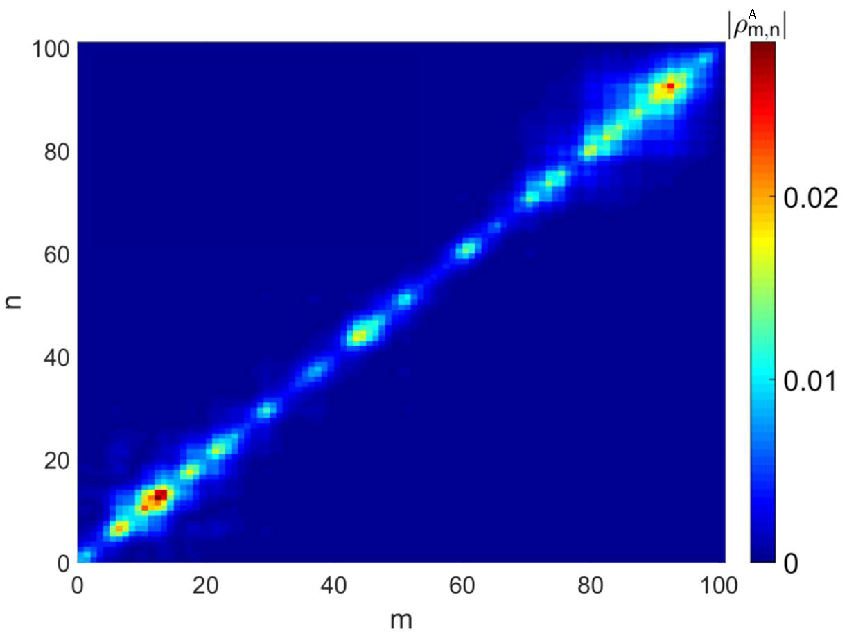
\includegraphics[width=0.5\linewidth]{anderson_rho_loc_1}}
		\hfill
		\subcaptionbox{\label{fig:anderson_rho_loc-2}}{%
			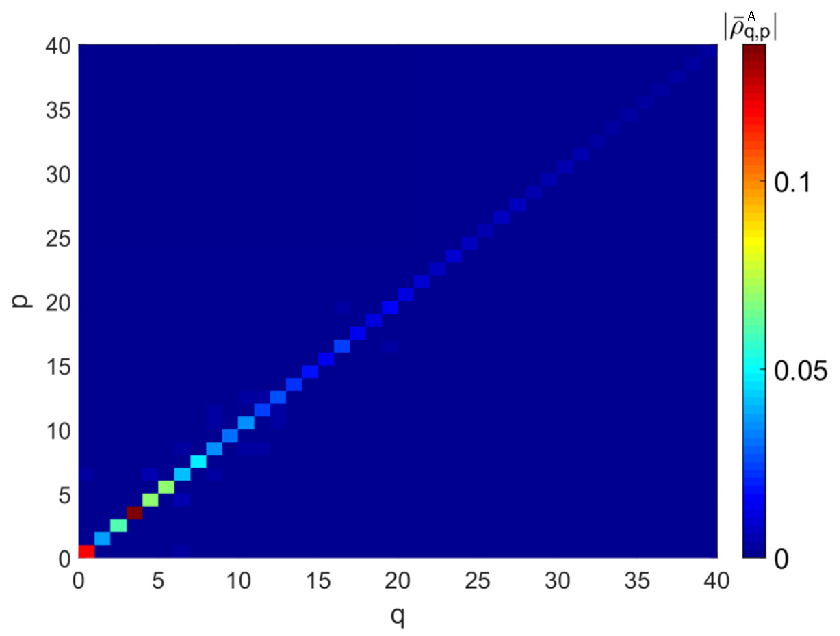
\includegraphics[width=0.5\linewidth]{anderson_rho_loc_2}}
		\hfill
	}
	\legend{}
	\caption[Асимптотическая матрица плотности с локализацией Андерсона]
	{
		Абсолютные значения асимптотической матрицы плотности \(\rho^A\) в исходном базисе (a) и в базисе собственных состояний модели Андерсона (б) для единичной реализации беспорядка. Использовались неэрмитовые диссипаторы \cref{eq:anderson_diss_local} c параметрами \(\alpha=0\) и \(l=1\). Сила пространственного беспорядка \(W=1\).
	}
	\label{fig:anderson_rho_loc}
\end{figure}

Зафиксируем параметры диссипаторов \(\alpha=0\) и \(l=1\) в формуле \cref{eq:anderson_diss_local} (синфазная диссипация на соседних сайтах решётки). В этом случае асимптотическая матрица плотности \(\rho^A\) имеет пятнистую структуру с несколькими яркими областями локализации, как показано на рисунке~\cref{fig:anderson_rho_loc-1}.
Рассмотрим асимптотическую матрицу плотности \(\rho^A\) в базисе собственных состояний модели Андерсона:
\begin{equation}
	\label{eq:anderson_rho_in_eigen_basis}
	\begin{gathered}
		\bar{\rho}^A = \mathcal{A}^\dagger \rho^A \mathcal{A},
	\end{gathered}
\end{equation}
где \(\mathcal{A} = \left(A_1 \ldots A_\nu \ldots A_N \right) \) "--- матрица собственных векторов гамильтониана \cref{eq:anderson_H}. В данном представлении матрица плотности \(\bar{\rho}^A\) является практически диагональной, с большим преобладанием значений из нижней части спектра, как показано на рисунке~\cref{fig:anderson_rho_loc-2}.

Для аналитического подтверждения данного наблюдения перепишем уравнение \cref{eq:GKSL_base} в базисе собственных состояний модели Андерсона \cref{eq:anderson_rho_in_eigen_basis}, пренебрегая недиагональными элементами матрицы плотности. В таком приближении эволюция диагональных элементов определяется только диссипативными членами:
\begin{equation}
	\label{eq:anderson_diag_mod_1}
	\begin{gathered}
		\dot{\bar{\rho}}_{p,p} = \gamma \left( \sum_q I_{p,q}\bar{\rho}_{q,q} - \bar{\rho}_{p,p} \sum_q I_{q,p} \right),
	\end{gathered}
\end{equation}
где коэффициенты перекрытий \(I_{p,q}\) представляются следующим образом через диссипативные операторы в базисе собственных состояний модели Андерсона (\(\bar{V}_k = \mathcal{A}^\dagger V_k \mathcal{A}\)):
\begin{equation}
	\label{eq:anderson_diag_mod_2}
	\begin{gathered}
		I_{p,q} = \sum_k \left| \left(\bar{V}_k\right)_{q,p} \right|^2 = \sum_k \left(\mathcal{A}_{p, k+l} + e^{i \alpha} \mathcal{A}_{p, k} \right)^2  \left(\mathcal{A}_{q, k+l} - e^{-i \alpha} \mathcal{A}_{q, k} \right)^2.
	\end{gathered}
\end{equation}
Система линейных дифференциальных уравнений \cref{eq:anderson_diag_mod_1} имеет единственное устойчивое состояние равновесия. Для его поиска, приравняем правую часть уравнения к \(0\), введём переобозначение:
\begin{equation}
	\label{eq:anderson_diag_mod_3}
	\begin{gathered}
		I^{\pm}_{p,k} = \left(\mathcal{A}_{p, k+l} \pm e^{\pm i \alpha} \mathcal{A}_{p, k} \right)^2 ,
	\end{gathered}
\end{equation}
и получим итоговое выражение для асимптотического состояния равновесия:
\begin{equation}
	\label{eq:anderson_diag_mod_4}
	\begin{gathered}
		\bar{\rho}^A_{p,p} = \frac{\sum_q I_{p,q}\bar{\rho}^A_{q,q}}{\sum_q I_{q,p}} = \frac{\sum_q \sum_k I^{+}_{p,k} I^{-}_{q,k} \bar{\rho}^A_{q,q}}{\sum_q \sum_k I^{+}_{q,k}  I^{-}_{p,k}} = \frac{\sum_k I^{+}_{p,k} \sum_q I^{-}_{q,k} \bar{\rho}^A_{q,q}}{ \sum_k I^{-}_{p,k} \sum_q  I^{+}_{q,k} } .
	\end{gathered}
\end{equation}
Внутренние суммы в числителе и знаменателе в самой правой части выражения не зависят от индекса \(p\). Они подвергаются усреднению по всем охватываемым собственным состояниям. Поскольку беспорядок пространственно однороден, среднее по ансамблю делает результат также независимым от индекса \(k\), и поэтому обе суммы соответствуют некоторой нормировочной константе. Таким образом, мы приходим к следующему выражению для асимптотической матрицы плотности в базисе собственных состояний модели Андерсона:
\begin{equation}
	\label{eq:anderson_diag_mod_5}
	\begin{gathered}
		\bar{\rho}^A_{p,p} \approx \frac{\sum_k I^{+}_{p,k}}{ \sum_k I^{-}_{p,k}}, 
	\end{gathered}
\end{equation}
которое полностью определяется типом диссипации и пространственной структурой конкретного собственного состояния.

Для случая синфазной диссипации на соседних сайтах решётки (\(\alpha=0\) и \(l=1\) в \cref{eq:anderson_diss_local}) получается соотношение:
\begin{equation}
	\label{eq:anderson_diag_mod_6}
	\begin{gathered}
		\sum_k \left( \mathcal{A}_{p, k+1} \pm \mathcal{A}_{p, k} \right)^2 = 2 \pm \sum_k \mathcal{A}_{p, k+1} \mathcal{A}_{p, k} = 2 \mp \lambda_p \mp \sum_k \varepsilon_k \mathcal{A}^2_{p, k}.
	\end{gathered}
\end{equation}
Оно основано на тождестве, полученном из следующего уравнения для собственных состояний:
\begin{equation}
	\label{eq:anderson_diag_mod_7}
	\begin{gathered}
		-\left( \lambda_p - \varepsilon_k \right) \mathcal{A}_{p, k} = \mathcal{A}_{p, k-1} + \mathcal{A}_{p, k+1},
	\end{gathered}
\end{equation}
которое, в свою очередь, умножается на \(\mathcal{A}_{p, k}\) и суммируется по \(k\).
В уравнении \cref{eq:anderson_diag_mod_6} в случае малого беспорядка (\(W < 4\)) и далеко от границ спектра, можно пренебречь последним слагаемым в правой части (усреднение из-за пространственного беспорядка), и в итоге получить следующее соотношение:
\begin{equation}
	\label{eq:anderson_diag_mod_8}
	\begin{gathered}
		\bar{\rho}^A_{p,p} \approx \frac{2-\lambda_p}{2+\lambda_p}.
	\end{gathered}
\end{equation}
Данный результат объясняет быстрое уменьшение вклада собственных состояний при отдалении от нижней границы спектра.
На рисунке~\cref{fig:anderson_rho_nn_1} для разных параметров силы беспорядка символами изображены усреднённые по многим реализация беспорядка распределения диагональных элементов асимптотической матрицы плотности в базисе собственных состояний модели Андерсона \(\bar{\rho}^A_{p,p}\) как функции усреднённых собственных значений. Количество реализаций беспорядка для усреднения: \(N_r=100\).
Полученные численные результаты хорошо согласуются с теоретической оценкой (формула \cref{eq:anderson_diag_mod_8} и фиолетовая кривая на рисунке~\cref{fig:anderson_rho_nn_1}). 
Несоответствие между результатами численных экспериментов и теоретической оценкой увеличивается с ростом силы беспорядка \(W\) и вблизи границ спектра "--- эти эффекты следуют из природы сделанных приближений.
\begin{figure}[ht]
	\centerfloat{
		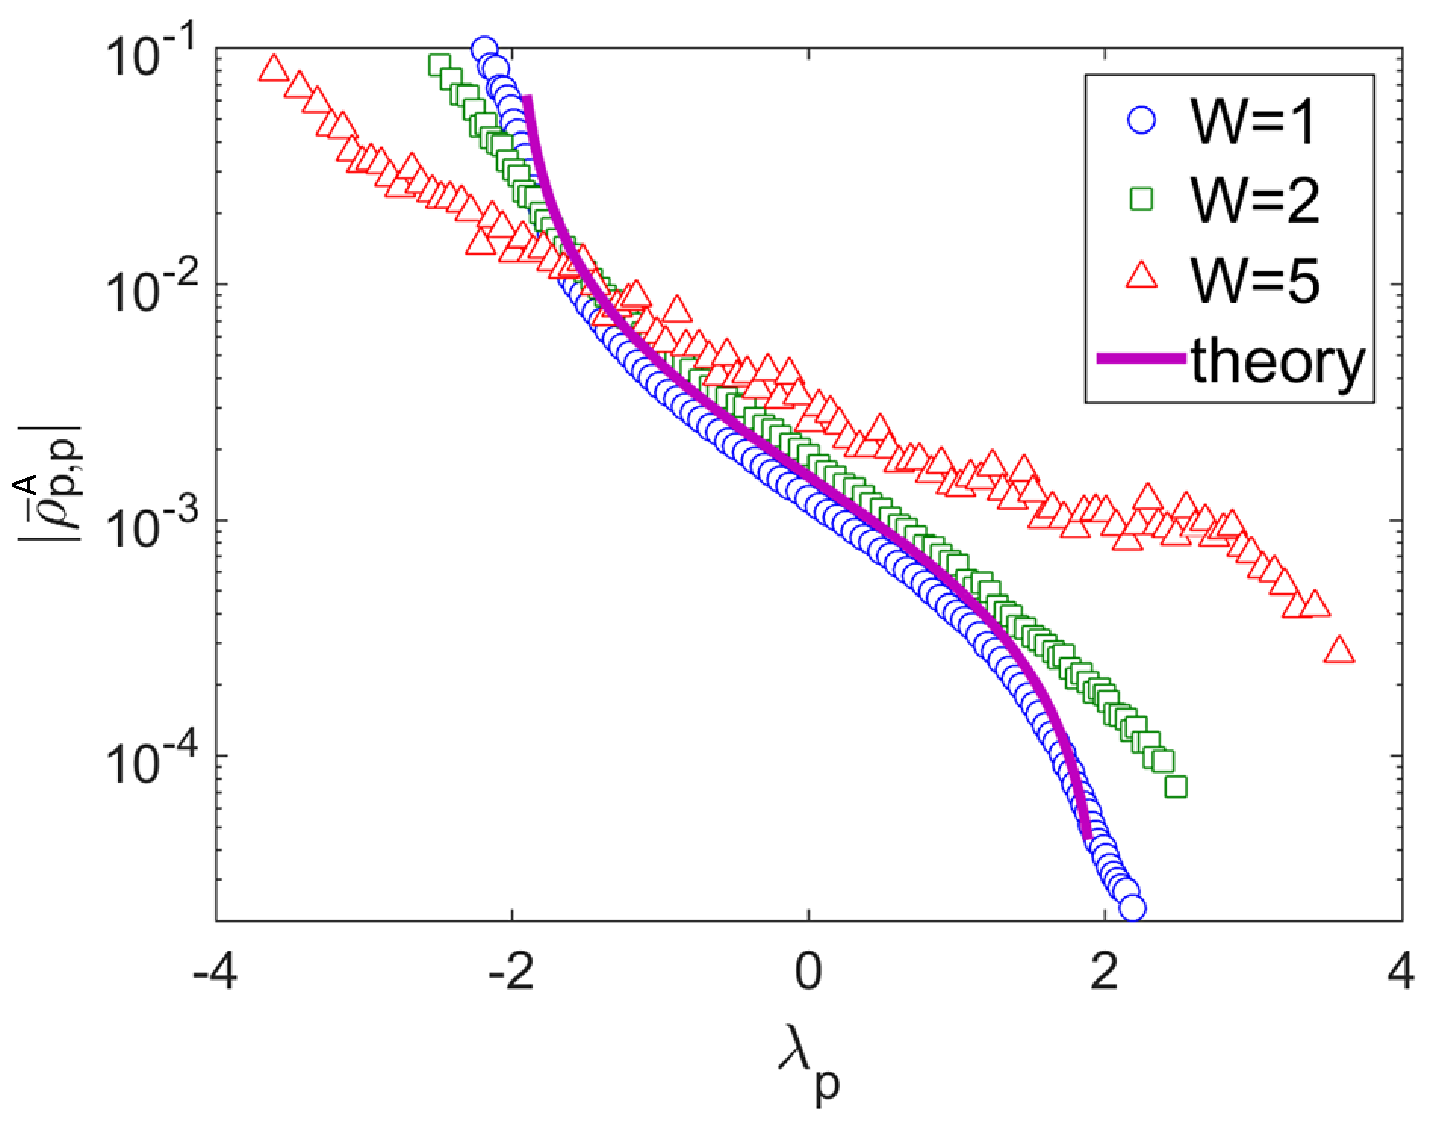
\includegraphics[scale=0.6]{anderson_rho_nn_1}
	}
	\caption[Усреднённые диагональные элементы матрицы плотности с локализацией Андерсона и теоретической оценкой]{
		Символы "--- усреднённые абсолютные значения диагональных элементов асимптотической матрицы плотности в базисе собственных состояний модели Андерсона как функции усреднённых собственных чисел для синфазной диссипации на соседних сайтах решётки (\(\alpha=0\) и \(l=1\) в уравнении \cref{eq:anderson_diss_local}) для разных значений беспорядка \(W\). Теоретический результат (формула \cref{eq:anderson_diag_mod_8}) показан фиолетовой сплошной линией.
	}
	\label{fig:anderson_rho_nn_1}
\end{figure}

Случай антифазной диссипации на соседних сайтах решетки (\(\alpha=\pi\) и \(l=1\) в уравнении \cref{eq:anderson_diss_local}), из-за симметрии, приводит к обратному выражению для формулы \cref{eq:anderson_diag_mod_8}:
\begin{equation}
	\label{eq:anderson_diag_mod_9}
	\begin{gathered}
		\bar{\rho}^A_{p,p} \approx \frac{2+\lambda_p}{2-\lambda_p}.
	\end{gathered}
\end{equation}
Асимптотическая матрица плотности является локализованной возле верхней границы спектра. 
При значениях фазы диссипации в промежутке \(0 < \alpha < \frac{\pi}{2}\)  в асимптотической матрице плотности в базисе собственных состояний модели Андерсона будут преобладать диагональные элементы, локализованные вблизи нижней границы спектра собственных значений. Аналогично, при значениях фазы диссипации в промежутке \(\frac{\pi}{2} < \alpha < \pi\) преобладают максимальные собственные значения из диапазона \cref{eq:anderson_evals}.

Качественно иная картина наблюдается для диссипативных операторов с \(\alpha=\pi\) и \(l=2\).
В этом случае асимптотическая матрица плотности в исходном базисе \(\rho^A\) является относительно более делокализованной (рисунок~\cref{fig:anderson_rho_loc-3}). 
В то же время, в базисе собственных состояний модели Андерсона \(\bar{\rho}^A\) \cref{eq:anderson_rho_in_eigen_basis} остаётся локализованной со смещением в центр спектра (рисунок~\cref{fig:anderson_rho_loc-4}).
\begin{figure}[ht]
	\centerfloat{
		\hfill
		\subcaptionbox[List-of-Figures entry]{\label{fig:anderson_rho_loc-3}}{%
			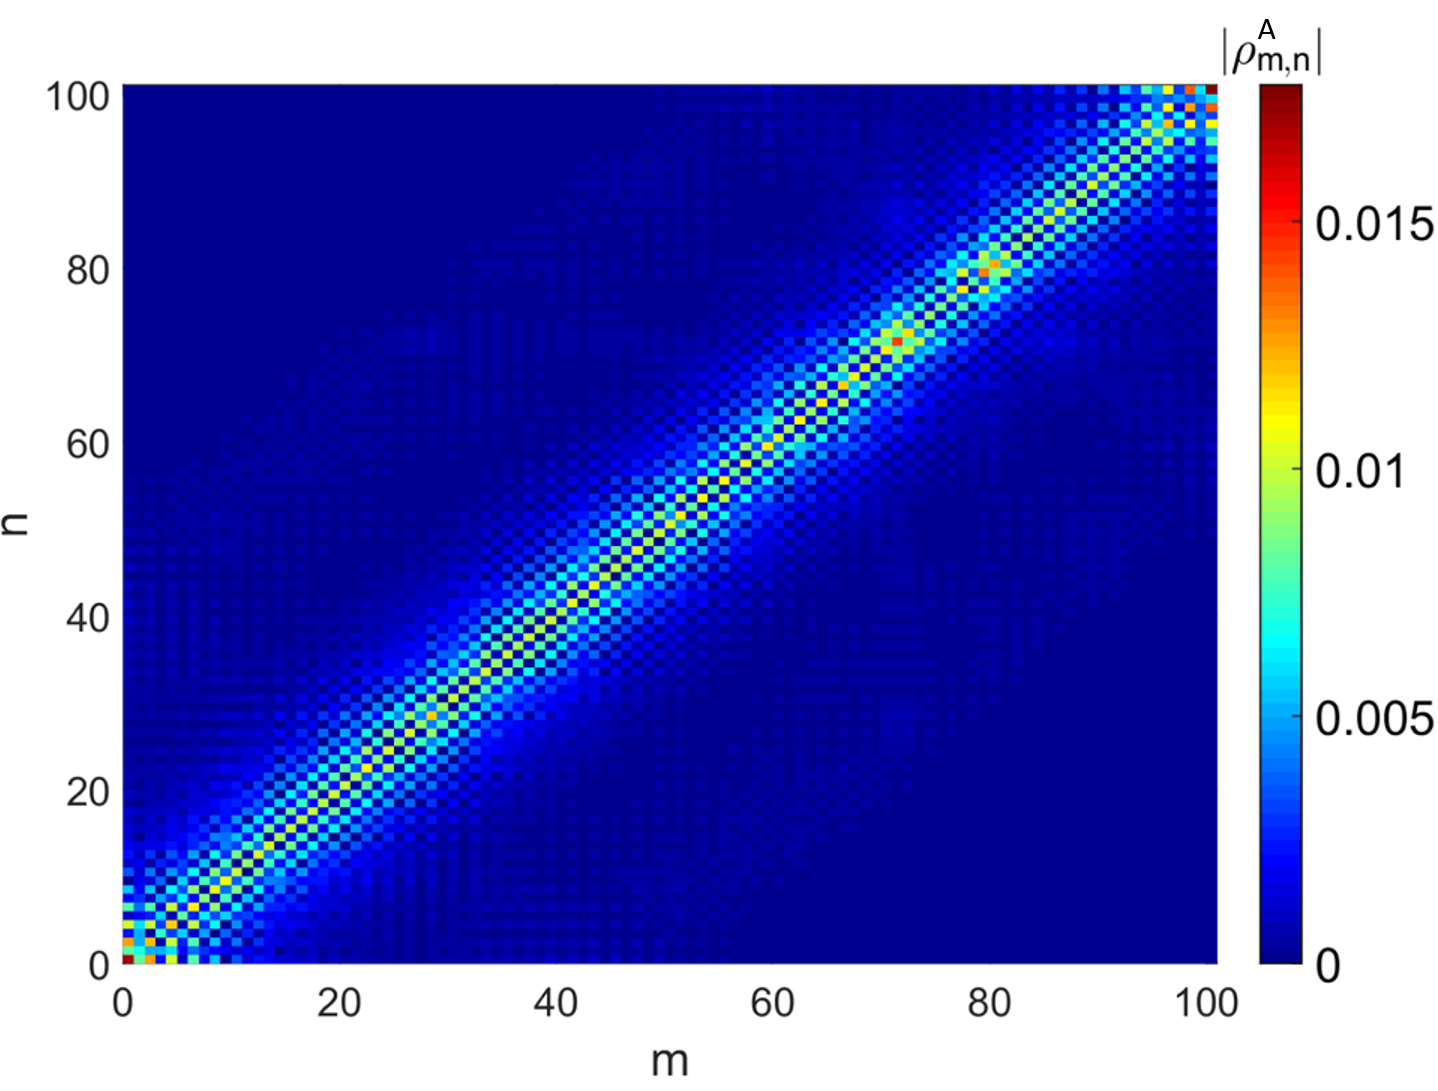
\includegraphics[width=0.5\linewidth]{anderson_rho_loc_3}}
		\hfill
		\subcaptionbox{\label{fig:anderson_rho_loc-4}}{%
			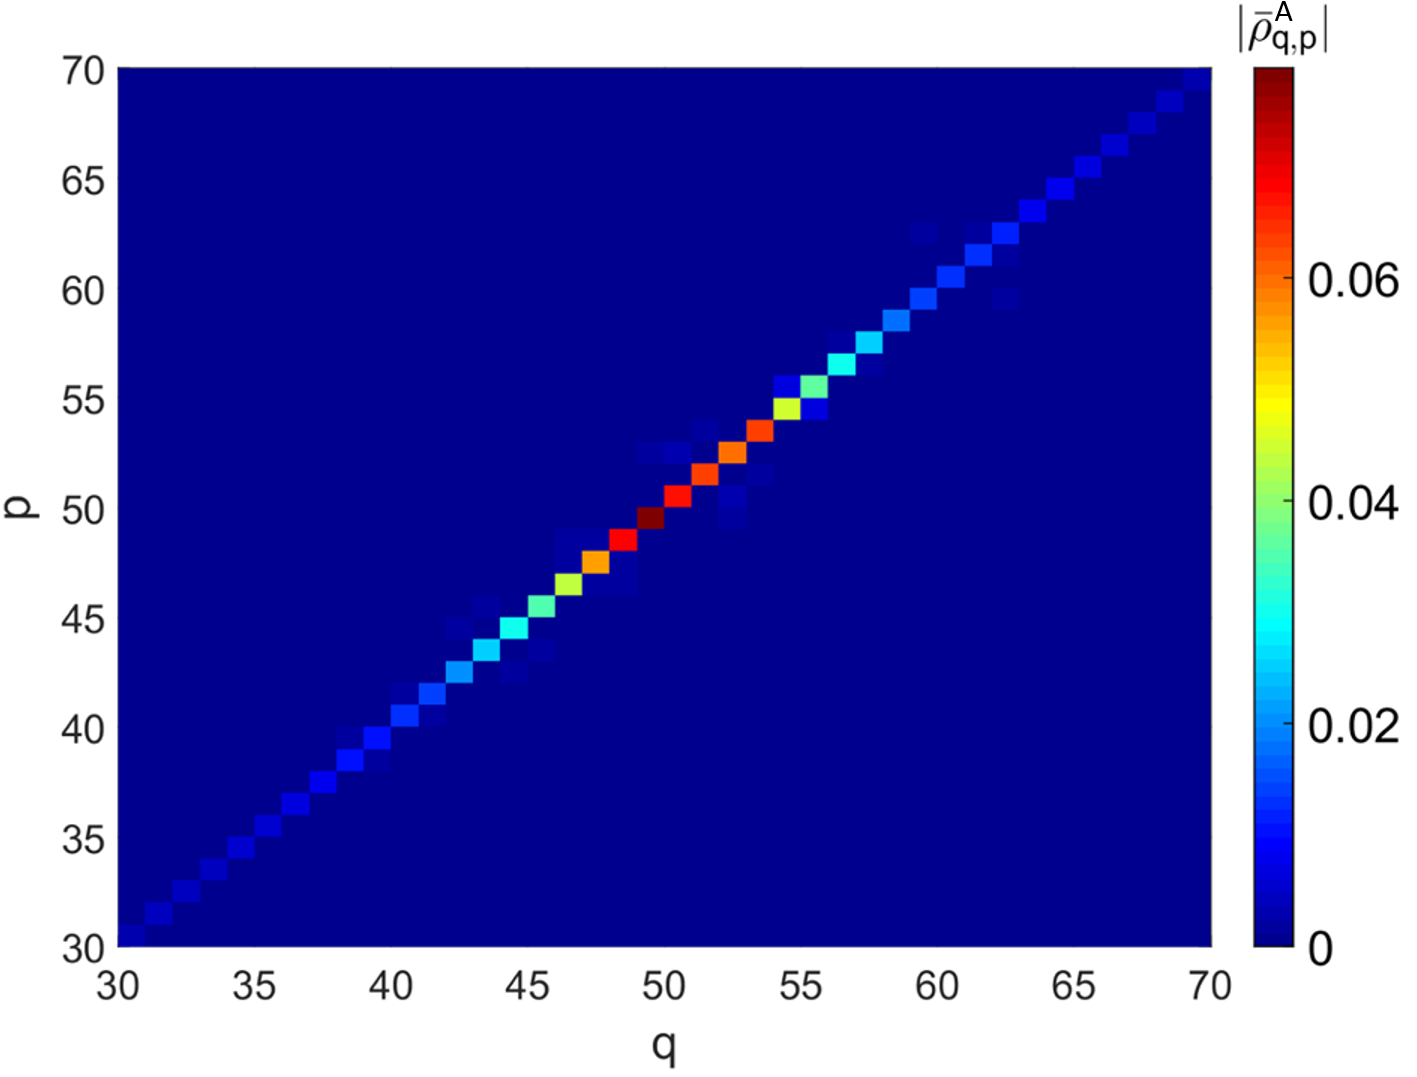
\includegraphics[width=0.5\linewidth]{anderson_rho_loc_4}}
		\hfill
	}
	\legend{}
	\caption[Асимптотическая матрица плотности с преобладанием делокализованных Андерсоновских мод]
	{
		Абсолютные значения асимптотической матрицы плотности \(\rho^A\) в исходном базисе (a) и в базисе собственных состояний модели Андерсона (б) для единичной реализации беспорядка. Использовались неэрмитовые диссипаторы \cref{eq:anderson_diss_local} c параметрами \(\alpha=\pi\) и \(l=2\). Сила пространственного беспорядка \(W=1\).
	}
	\label{fig:anderson_rho_loc_mid}
\end{figure}
Относительная делокализация в исходном базисе вызвана существенным вкладом собственных состояний из центра спектра, которые имеют относительно большую длину локализации \cref{eq:anderson_loc_length}.
Аналитические соотношения для данного случая выглядят следующим образом:
\begin{equation}
	\label{eq:anderson_diag_mod_10}
	\begin{gathered}
		I^{-}_p = \sum_{k} \left( \mathcal{A}_{p, k+2} \pm \mathcal{A}_{p, k} \right)^2 = \\
		= \lambda^2 - 2 \lambda_p \sum_{k} \varepsilon_k \mathcal{A}_{p, k} \mathcal{A}_{p, k+1} + \sum_{k} \varepsilon^2_k \mathcal{A}^2_{p, k} \approx \lambda^2_p + \frac{W^2}{12}, \\
		I^{+}_p = 4 - I^{-}_p,
	\end{gathered}
\end{equation}
которые в итоге приводят к следующему выражению для диагональных элементов матрицы плотности в базисе собственных состояний модели Андерсона:
\begin{equation}
	\label{eq:anderson_diag_mod_11}
	\begin{gathered}
		\bar{\rho}^A_{p,p} \approx \frac{4}{\lambda^2_p + \frac{W^2}{12}} - 1.
	\end{gathered}
\end{equation}
Данное выражение указывает на то, что наибольший вклад в решение вносят собственные состояния из центра спектра.
На рисунке \cref{fig:anderson_rho_nn_2} изображены усреднённые по \(N_r=100\) случайным реализациям беспорядка диагональные элементы матрицы плотности в базисе собственных состояний модели Андерсона для разных значений силы беспорядка вместе с аналитическим результатом \cref {eq:anderson_diag_mod_11} (сплошные линии). На графике видно хорошее соответствие между численными и аналитическими результатами при малом беспорядке \(W\). При увеличении \(W\) несоответствие увеличивается на краях спектра \(\lambda_p\) ввиду сделанных теоретических приближений. 
\begin{figure}[ht]
	\centerfloat{
		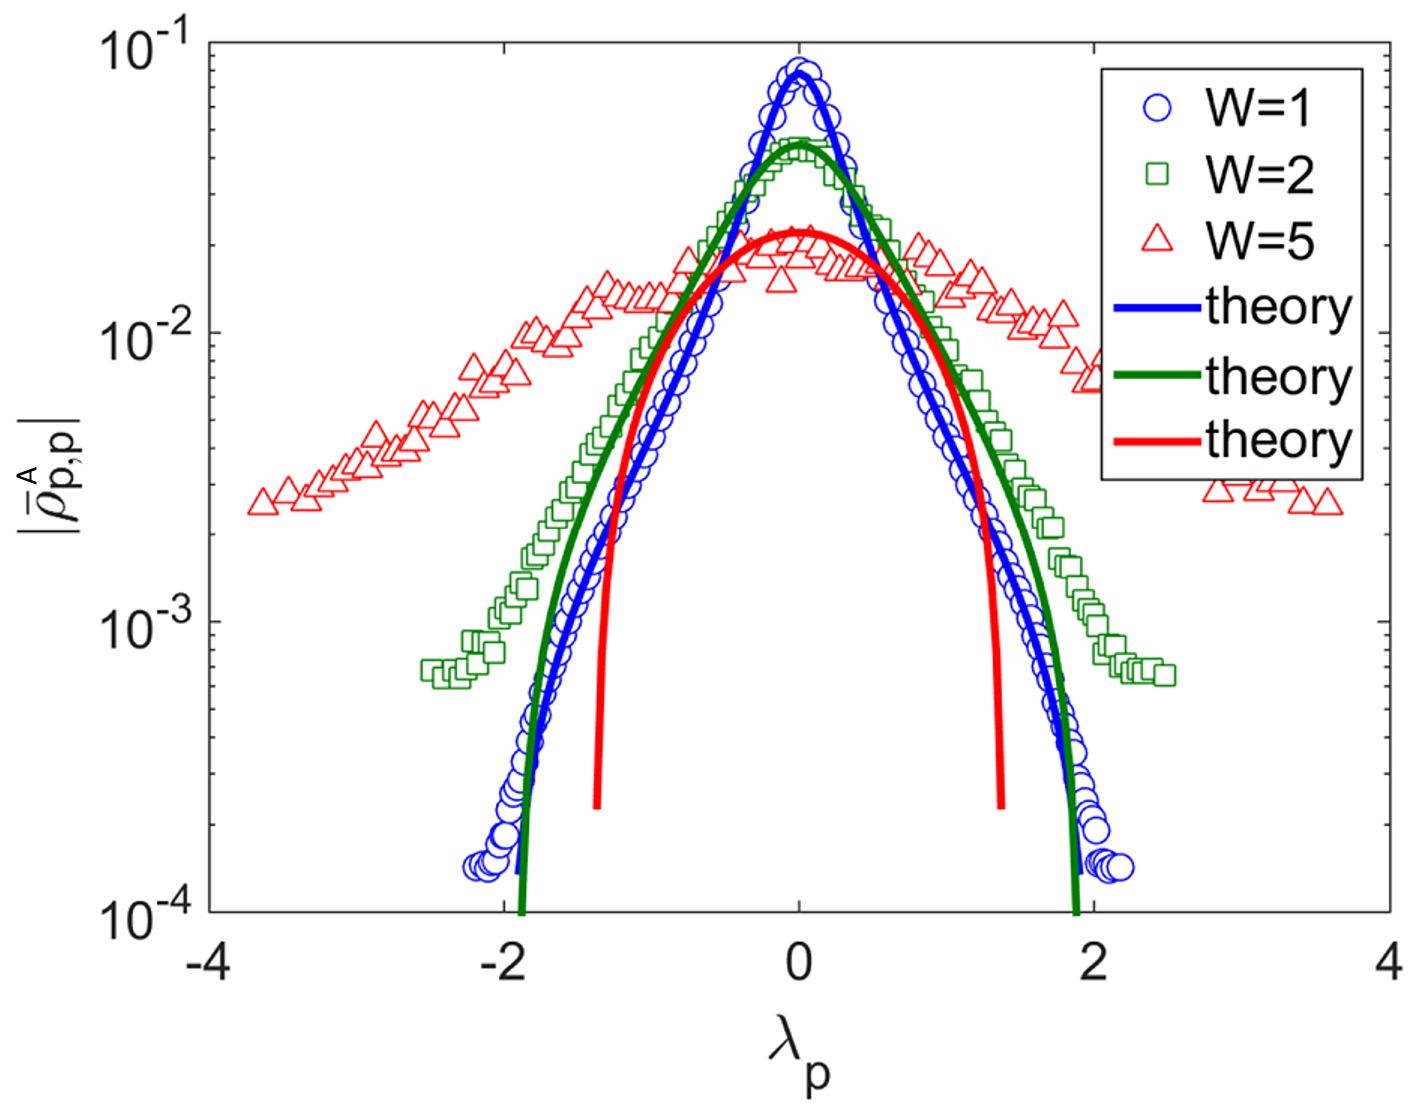
\includegraphics[scale=0.4]{anderson_rho_nn_2}
	}
	\caption[Усреднённые диагональные элементы матрицы плотности c преобладанием делокализованных Андерсоновских мод и теоретической оценкой]{
		Символы "--- усреднённые абсолютные значения диагональных элементов асимптотической матрицы плотности в базисе собственных состояний модели Андерсона как функции усреднённых собственных чисел для неэрмитовой диссипации  с \(\alpha=\pi\) и \(l=2\) в уравнении \cref{eq:anderson_diss_local} для разных значений беспорядка \(W\). Теоретический результат \cref{eq:anderson_diag_mod_11} для каждого значения \(W\) показан соответствующей сплошной линией.
	}
	\label{fig:anderson_rho_nn_2}
\end{figure}

Рассмотрим открытую модель Андерсона \cref{eq:GKSL_lindbladian, eq:anderson_H, eq:anderson_diss_local} c микроскопической точки зрения, используя метод квантовых тректорий, описанный в разделе \cref{sec:ch1/qj}. Квантовая траектория с индексом \(j\) будет описываться волновой функцией \(\left| \psi_j(t) \right\rangle\). Зафиксируем случайный беспорядок в системе силой \(W=1\) и время переходного процесса \(t^A = 10^4\) "--- достаточным до достижения каждой траекторией аттрактора (асимптотической матрицы плотности \(\rho^A\)). После достижения аттрактора за каждой квантовой траекторией будет вестись наблюдение в течении \(t^O = 10^4\) (суммарное время пропагации \(t = t^A + t^O\)). Количество рассматриваемых квантовых траекторий \(M_r=10^6\). Для каждой \(j\)-ой квантовой траектории будут рассматриваться позиция и энергия, вычисляемые по соответствующим формулам:
\begin{equation}
	\label{eq:anderson_position}
	\begin{gathered}
		n_j(t) = \langle \psi_j(t)| O_n | \psi_j(t) \rangle,
	\end{gathered}
\end{equation}
\begin{equation}
	\label{eq:anderson_energy}
	\begin{gathered}
		E_j(t) = \langle \psi_j(t)| H | \psi_j(t) \rangle,
	\end{gathered}
\end{equation}
где \(O_n\) - матрица оператора числа частиц, а \(H\) - гамильтониан модели Андерсона \cref{eq:anderson_H}.

\begin{figure}[ht]
	\centerfloat{
		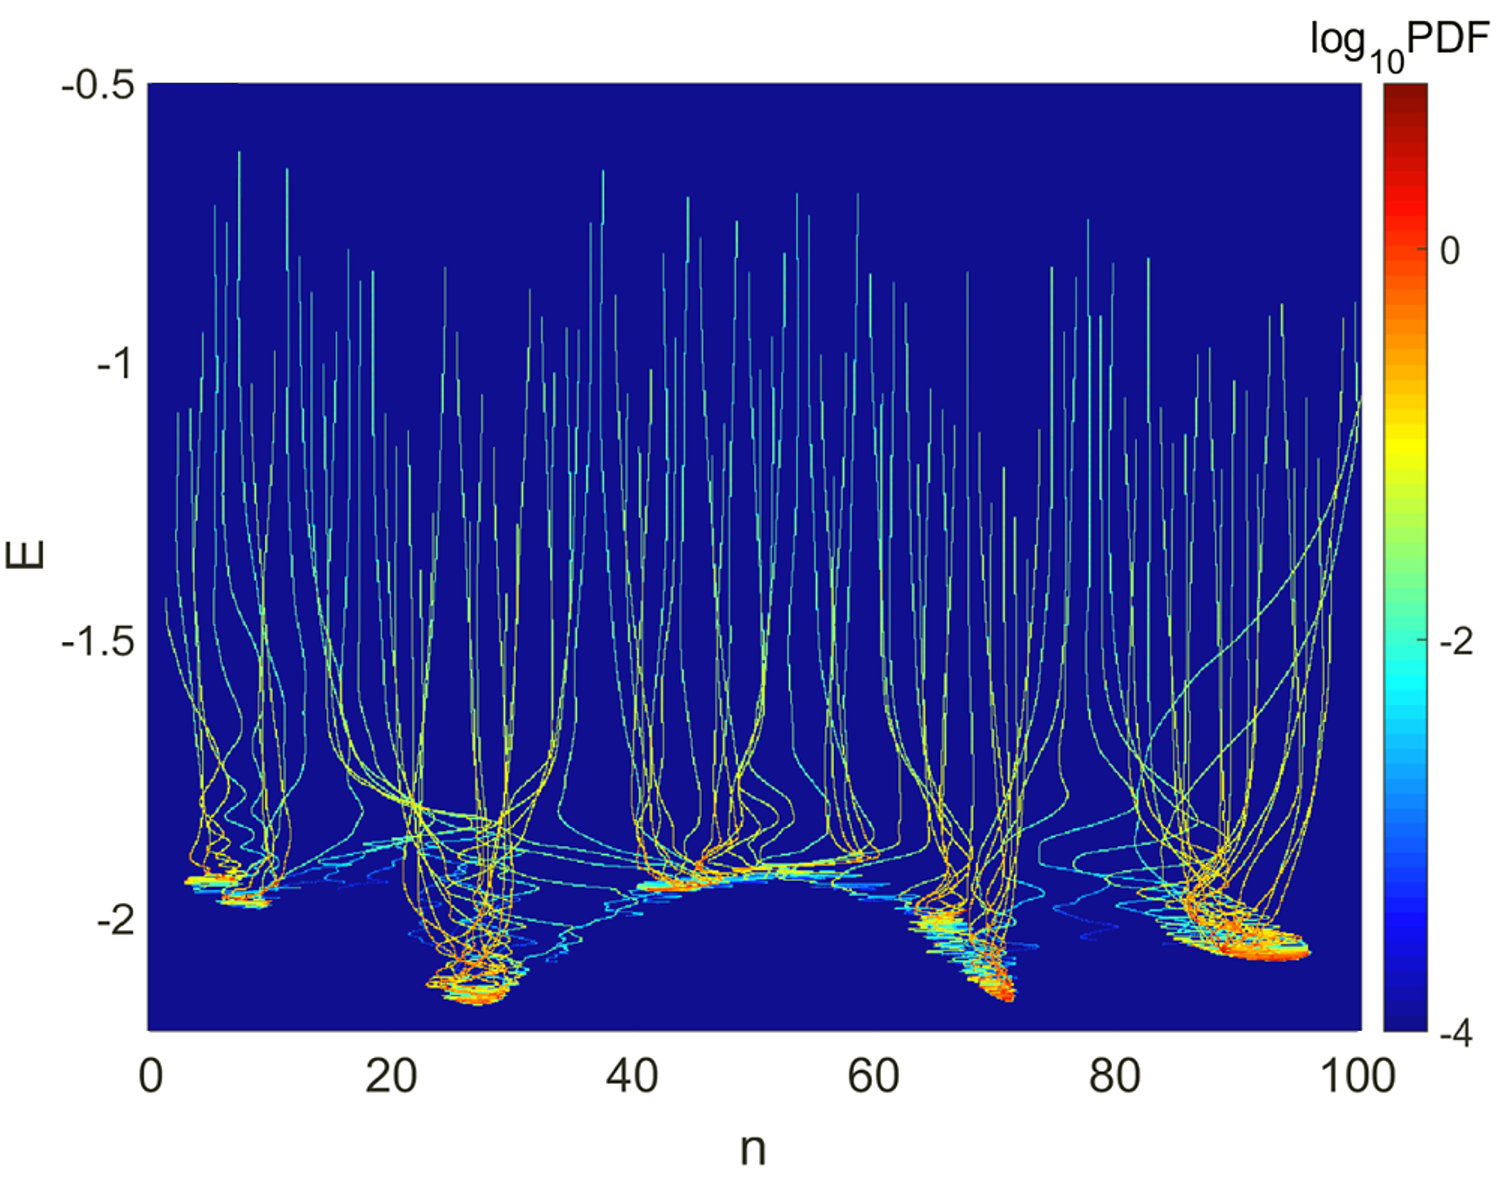
\includegraphics[scale=0.4]{anderson_qj_1}
	}
	\caption[Плотность вероятностей квантовых траекторий на плоскости позиции и энергий в случае  локализации Андерсона]{
		Функция распределения плотности вероятностей (PDF) квантовых траекторий на плоскости позиции \(n(t)\) и энергии \(E(t)\) для случая синфазной диссипации на соседних сайтах решётки (\(\alpha=0\) и \(l=1\) в \cref{eq:anderson_diss_local}).
	}
	\label{fig:anderson_qj_1}
\end{figure}

На рисунке \cref{fig:anderson_qj_1} изображена двумерная функция распределения плотности вероятностей (probability densidy function - PDF) на плоскости позиции \(n(t)\) \cref{eq:anderson_position} и энергии \(E(t)\) \cref{eq:anderson_energy} , построенная для \(M_r=10^6\) траекторий, наблюдаемых в течение \(t^O=10^4\) времени для случая синфазной диссипации на соседних сайтах решётки (\(\alpha=0\) и \(l=1\) в \cref{eq:anderson_diss_local}). Динамика отдельных квантовых траекторий представляет собой длительные «залипания» вблизи центров локализации (красные области на рисунке \cref{fig:anderson_qj_1}), вызванные эволюцией с неэрмитовым гамильтонианом \cref{eq:H_nonhermit} (алгоритм \ref{alg:qt_main}). Данные процессы прерываются квантовыми скачками (алгоритм \ref{alg:qt_jump}), которые накачивают систему энергией и переносят траектории в бледно-голубые «истоки» сети в верхней части рисунка \cref{fig:anderson_qj_1}, откуда системы быстро релаксирует по структурированной сети к одному из собственных состояний модели Андерсона. Структура сети не меняется при дальнейшем увеличении числа траекторий \(M_r\).

Результаты \cite{Yusipov2017}, представленные в данном разделе, указывают на то, что в открытых квантовых системах с физически реализуемой диссипацией возможно создание стационарных состояний, в которых доминируют несколько локализованных мод пространственно неоднородного гамильтониана из классической модели Андерсона. Андерсоновские моды выбираются в соответствии с их пространственно-фазовыми свойствами, унаследованными от собственных состояний гамильтониана в пределе нулевого беспорядка \cite{Ishii1973}, с использованием фазо"--~параметризованных диссипативных операторов. Изменение фазы диссипативных операторов изменяет локализационные свойства системы.

\section{Управление одночастичной локализацией в открытых квантовых системах}\label{sec:ch2/epjb}
В данном разделе будет изучено влияние параметров диссипативных операторов \cref{eq:anderson_diss_local} на локализационные свойства открытой квантовой системы \cref{eq:GKSL_lindbladian,eq:anderson_H}, а также влияние добавочной дефазирующей диссипации \cref{eq:anderson_diss_dephase} на асимптотическое состояние системы.

Рассмотрим случай синфазной диссипации на соседних сайтах решётки (\(\alpha=0\) и \(l=1\) в \cref{eq:anderson_diss_local} с коэффициентами скорости диссипации \(\gamma^l = 0.1\). Добавим к данной модели дополнительные дефазирующие \cref{eq:anderson_diss_dephase} каналы рассеивания с коэффициентами скорости \(\gamma^d\). На рисунке \cref{fig:anderson_rho_nn_with_dephasing} изображены диагональные элементы асимптотической матрицы плотности в базисе собственных состояний модели Андерсона со смешанным типом диссипации для разных значений \(\gamma^d\). Стоить отметить, что не только слабая \(\gamma^d \ll \gamma^l\), но и сильная \(\gamma^d \gg \gamma^l\) дефазирующая диссипация не уничтожает спектральную диссипацию и структурно не изменяет решение (преобладают собственные состояния из той же части спектра).

\begin{figure}[ht]
	\centerfloat{
		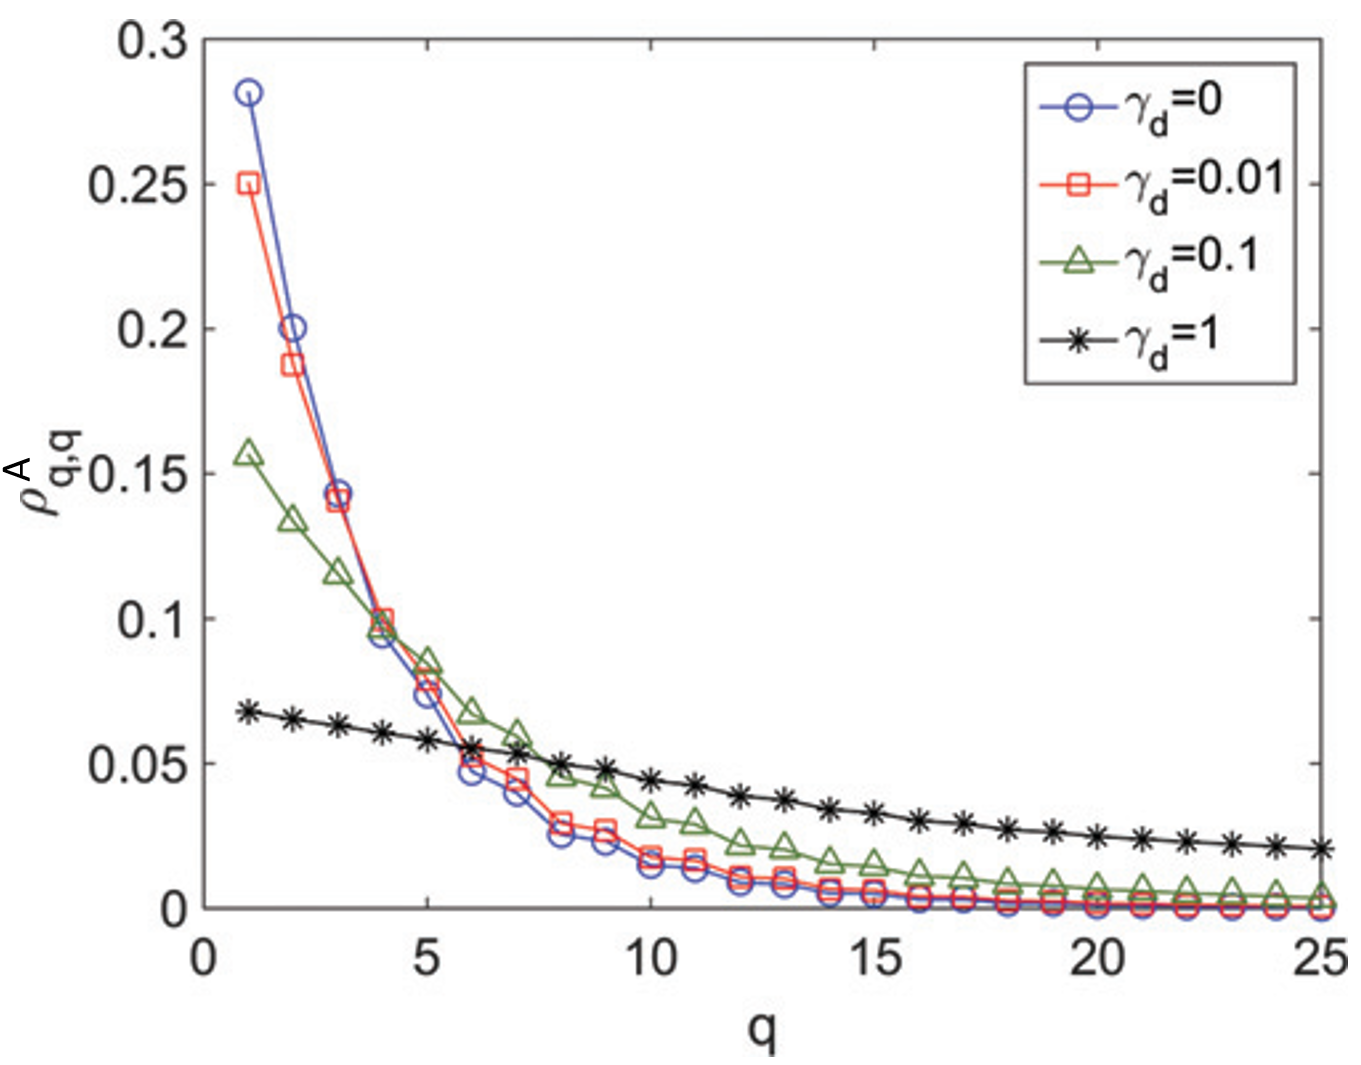
\includegraphics[scale=0.4]{anderson_rho_nn_with_dephasing}
	}
	\caption[Диагональные элементы асимптотической матрицы плотности в базисе собственных состояний модели Андерсона для разных типов диссипации]{
		Диагональные элементы асимптотической матрицы плотности в базисе собственных состояний модели Андерсона \(\bar{\rho}^A\) для случая синфазной диссипации на соседних сайтах решётки (\(\alpha=0\) и \(l=1\) в \cref{eq:anderson_diss_local} и скорость диссипации \(\gamma^l=0.1\)) в комбинации с дефазирующей диссипацией (\cref{eq:anderson_diss_dephase} и скорость диссипации \(\gamma^d\)) для разных значений \(\gamma^d\). Размер решётки \(N=25\), сила пространственного беспорядка \(W=2\). Усреднение производилось для \(N_r = 10^3\) реализаций беспорядка. 
	}
	\label{fig:anderson_rho_nn_with_dephasing}
\end{figure}

Рассмотрим теперь систему в пределе нулевого беспорядка. Базис системы состоит из плоских волн с соответсвующим спектром собственных значений:
\begin{equation}
	\label{eq:anderson_plane_wave}
	\begin{gathered}
		\phi_j = \frac{e^{i j k}}{\sqrt{N}}, \\
		\lambda_k = -2 \cos{k}, \\
		k = \frac{2 \pi q}{N}, \\
		q = -\frac{N}{2}, \ldots, \frac{N}{2}.
	\end{gathered}
\end{equation}
Можно заметить, что для конкретного значения фазы диссипатора \cref{eq:anderson_diss_local} \(\alpha = \frac{2 \pi q}{N}\), плоская волна  \cref{eq:anderson_plane_wave} с соответствующим \(k=\alpha\) является «тёмным» состоянием для всех диссипативных операторов \cref{eq:anderson_diss_local} \cite{Diehl2008, Kraus2008}, в то время как все остальные собственные состояния не являются.
В этом случае (когда нет дефазирующей добавки \(\gamma^d = 0\)), плоская волна с \(k = \alpha\) является асимптотическим состоянием открытой квантовой системы. 
В том случае, когда \(\alpha\) не совпадает точно со значением \(k\) или присутствует дефазирующая диссипация, асимптотическое состояние остаётся очень близким к исходному «тёмному» состоянию, причём наибольший вклад вносят плоские волны с \(k \approx \alpha\) (рисунок \cref{fig:anderson_rho_nn_zero_disorder}).
\begin{figure}[ht]
	\centerfloat{
		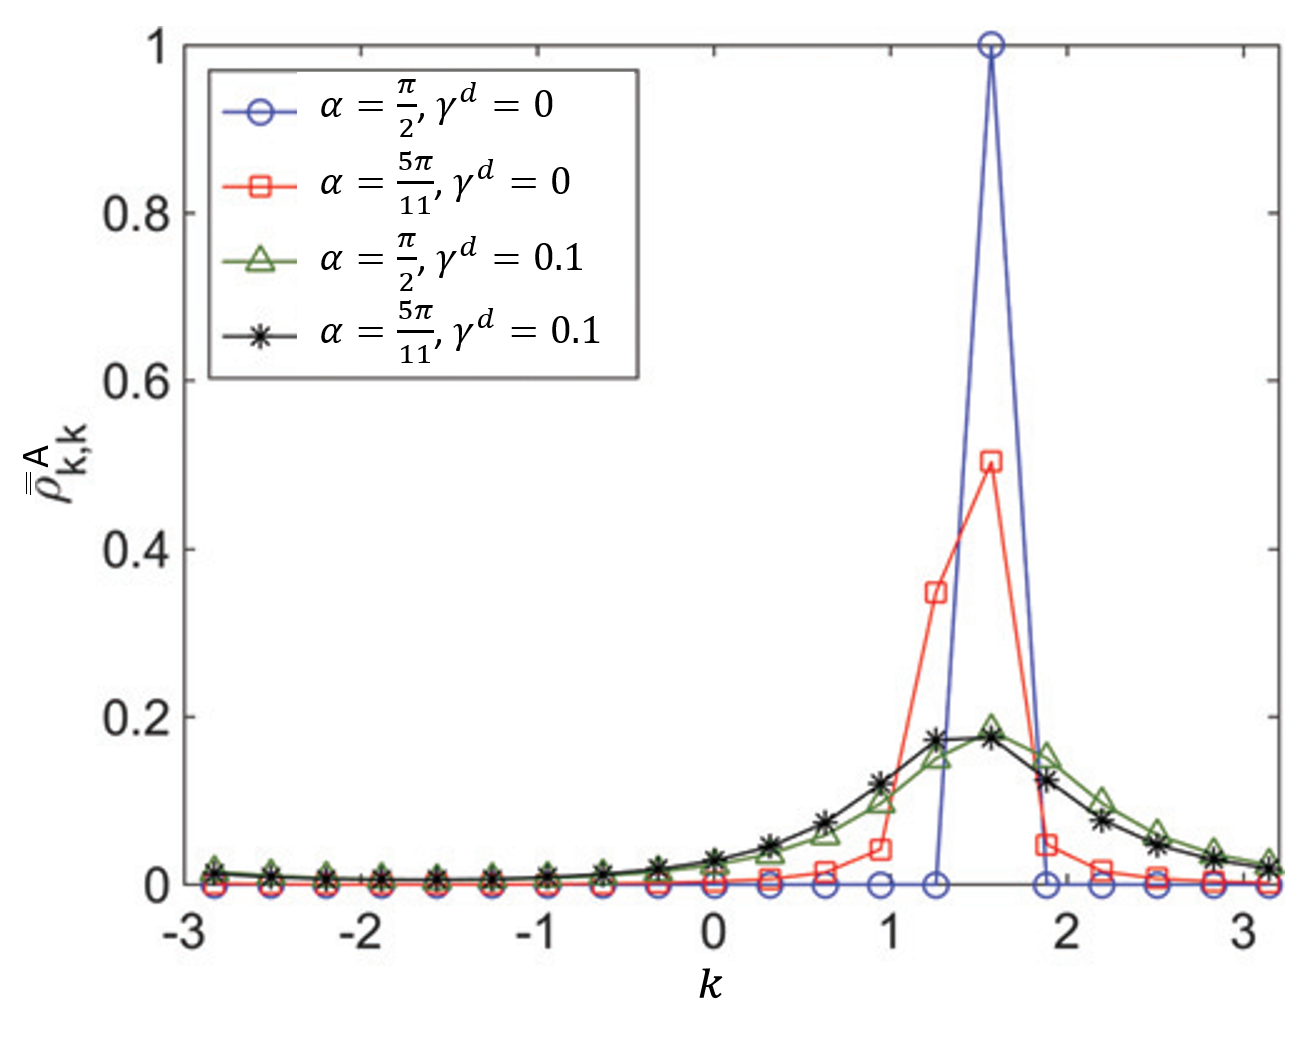
\includegraphics[scale=0.4]{anderson_rho_nn_zero_disorder}
	}
	\caption[Диагональные элементы асимптотической матрицы плотности в базисе Андерсоновских мод при нулевом беспорядке в зависимости от разных типов диссипации]{
		Диагональные элементы асимптотической матрицы плотности в базисе плоских волн \(\bar{\bar{\rho}}^A_{k,k}\) \cref{eq:anderson_plane_wave} для случая синфазной диссипации на соседних сайтах решётки (\(\alpha=0\) и \(l=1\) в \cref{eq:anderson_diss_local} и скорость диссипации \(\gamma^l=0.1\)) в комбинации с дефазирующей диссипацией (\cref{eq:anderson_diss_dephase} и скорость диссипации \(\gamma^d\)). Размер решётки \(N=20\), сила пространственного беспорядка \(W=0\).
	}
	\label{fig:anderson_rho_nn_zero_disorder}
\end{figure}

Ненулевой беспорядок \(W\) приводит к локализации Андерсона всех собственных состояний данной модели, которые при этом перестают в точности быть «тёмными» состояниями соответствующих диссипаторов \cref{eq:anderson_diss_local}.
Однако, известно, что моды Андерсона наследуют фазовые свойства исходных плоских волн (по крайней мере, в режиме слабого беспорядка), хотя их амплитуды экспоненциально затухают в пространстве \cite{Ishii1973}.
Следовательно, избирательный эффект неэрмитовых диссипаторов \cref{eq:anderson_diss_local} сохраняется.
\begin{figure}[h]
	\centerfloat{
		\hfill
		\subcaptionbox[List-of-Figures entry]{\label{fig:anderson_modes_in_foutier_1_1}}{%
			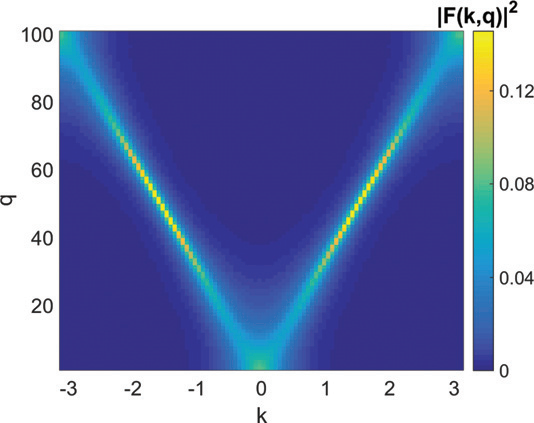
\includegraphics[width=0.45\linewidth]{anderson_modes_in_fourier_1_1}}
		\hfill
		\subcaptionbox{\label{fig:anderson_modes_in_foutier_1_2}}{%
			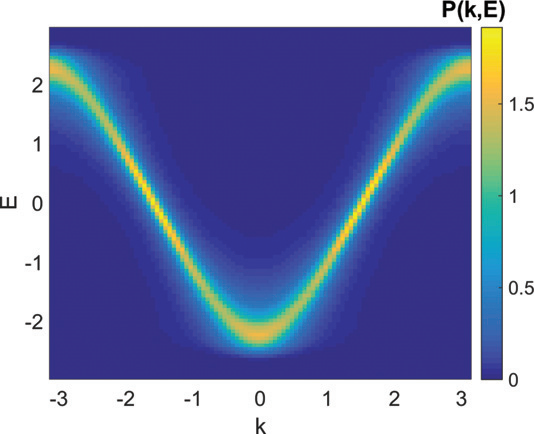
\includegraphics[width=0.45\linewidth]{anderson_modes_in_fourier_1_2}}
		\hfill
	}
	\legend{}
	\caption[Анализ Андерсоновских мод в Фурье"--~базисе для слабого беспорядка]
	{
		Собственные состояния модели Андерсона (Андерсоновские моды) с беспорядком \(W=2\) в Фурье"--~базисе плоских волн \cref{eq:anderson_modes_in_plane_wave}. (а): квадрат значения гармоник \(\left| F(k,q) \right|^2\) в зависимости от волнового числа \(k\) и номера моды \(q\); (б): значения спектральной плотности \(P(k,E)\) \cref{eq:anderson_modes_in_plane_wave_density}.
	}
	\label{fig:anderson_modes_in_foutier_1}
\end{figure}
\begin{figure}[h]
	\centerfloat{
		\hfill
		\subcaptionbox[List-of-Figures entry]{\label{fig:anderson_modes_in_foutier_2_1}}{%
			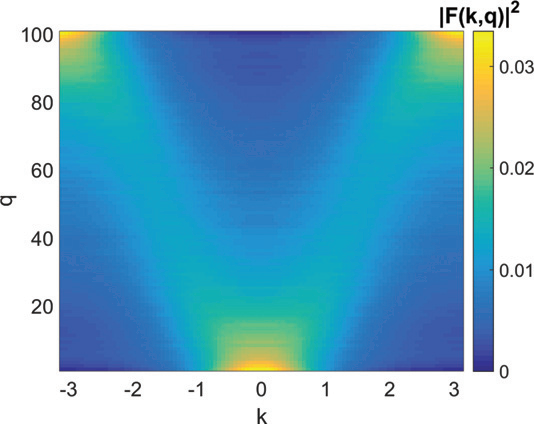
\includegraphics[width=0.45\linewidth]{anderson_modes_in_fourier_2_1}}
		\hfill
		\subcaptionbox{\label{fig:anderson_modes_in_foutier_2_2}}{%
			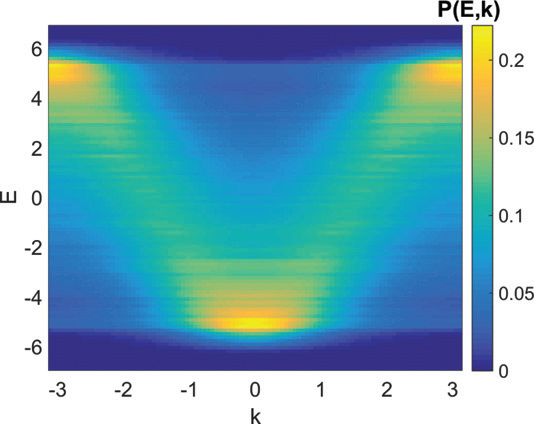
\includegraphics[width=0.45\linewidth]{anderson_modes_in_fourier_2_2}}
		\hfill
	}
	\legend{}
	\caption[Анализ Андерсоновских мод в Фурье"--~базисе для сильного беспорядка]
	{
		Собственные состояния модели Андерсона (Андерсоновские моды) с беспорядком \(W=10\) в Фурье"--~базисе плоских волн \cref{eq:anderson_modes_in_plane_wave}. (а): квадрат значения гармоник \(\left| F(k,q) \right|^2\) в зависимости от волнового числа \(k\) и номера моды \(q\); (б): значения спектральной плотности \(P(k,E)\) \cref{eq:anderson_modes_in_plane_wave_density}.
	}
	\label{fig:anderson_modes_in_foutier_2}
\end{figure}
\begin{figure}[h]
	\centerfloat{
		\hfill
		\subcaptionbox[List-of-Figures entry]{\label{fig:anderson_rho_kk_in_foutier_1_1}}{%
			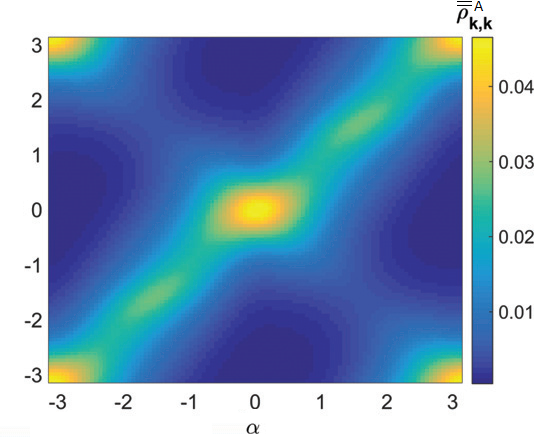
\includegraphics[width=0.45\linewidth]{anderson_rho_kk_in_foutier_1_1}}
		\hfill
		\subcaptionbox{\label{fig:anderson_rho_kk_in_foutier_1_2}}{%
			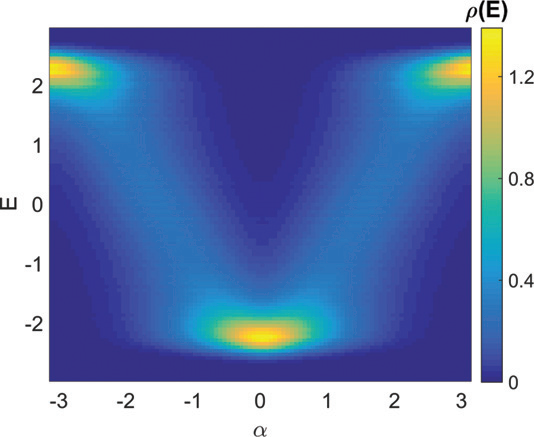
\includegraphics[width=0.45\linewidth]{anderson_rho_kk_in_foutier_1_2}}
	}
	\legend{}
	\caption[Асимптотическое состояние открытой системы Андерсона для слабого беспорядка в зависимости от параметра диссипации]
	{
		Асимптотическое состояние открытой системы Андерсона с беспорядком \(W=2\) и усреднением по \(N_r=10^3\) реализаций беспорядка в зависимости от параметра диссипации \(\alpha\) (\cref{eq:anderson_diss_local}). (а): диагональные элементы асимптотической матрицы плотности в базисе плоских волн \(\rho^A_{k,k}\) \cref{eq:anderson_plane_wave} ; (б): спектральная плотность диагональных элементов матрицы плотности в базисе собственных состояний модели Андерсона.
	}
	\label{fig:anderson_rho_kk_in_foutier_1}
\end{figure}
\begin{figure}[h]
	\centerfloat{
		\hfill
		\subcaptionbox[List-of-Figures entry]{\label{fig:anderson_rho_kk_in_foutier_2_1}}{%
			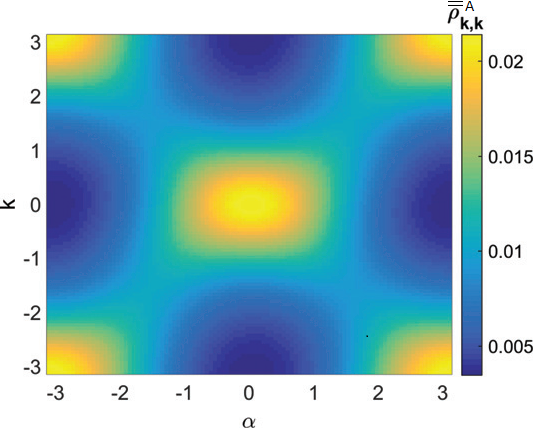
\includegraphics[width=0.45\linewidth]{anderson_rho_kk_in_foutier_2_1}}
		\hfill
		\subcaptionbox{\label{fig:anderson_rho_kk_in_foutier_2_2}}{%
			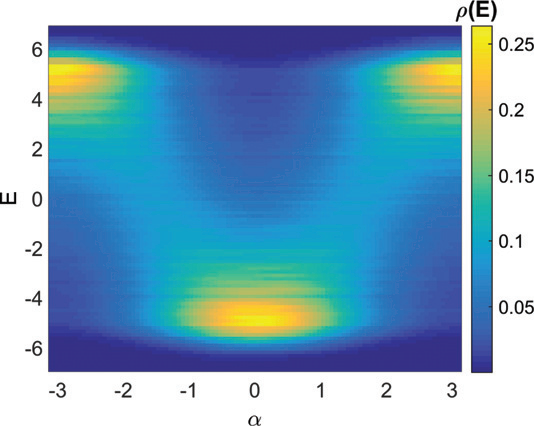
\includegraphics[width=0.45\linewidth]{anderson_rho_kk_in_foutier_2_2}}
	}
	\legend{}
	\caption[Асимптотическое состояние открытой системы Андерсона для сильного беспорядка в зависимости от параметра диссипации]
	{
		Асимптотическое состояние открытой системы Андерсона с беспорядком \(W=10\) и усреднением по \(N_r=10^3\) реализаций беспорядка в зависимости от параметра диссипации \(\alpha\) (\cref{eq:anderson_diss_local}). (а): диагональные элементы асимптотической матрицы плотности в базисе плоских волн \(\rho^A_{k,k}\) \cref{eq:anderson_plane_wave} ; (б): спектральная плотность диагональных элементов матрицы плотности в базисе собственных состояний модели Андерсона.
	}
	\label{fig:anderson_rho_kk_in_foutier_2}
\end{figure}

Зафиксируем параметры системы \(\gamma^l = \gamma^d = 0.1\), \(N=100\) и проанализируем структуру Андерсоновских мод \(A^{q}_k\) в базисе плоских волн \cref{eq:anderson_plane_wave} (Фурье"--~базис) для разных значений силы беспорядка \(W\).
Несмотря на то, что экспоненциальная локализация в прямом пространстве предполагает делокализацию в базисе плоских волн, она не исключает неоднородности распределения в нем.
Коэффициенты разложения, которые выражаются следующим образом:
\begin{equation}
	\label{eq:anderson_modes_in_plane_wave}
	\begin{gathered}
		F(k,q) = \sum A^q_k \frac{e^{i j k}}{\sqrt{N}},
	\end{gathered}
\end{equation}
имеют ярко выраженные максимумы вдоль линейных зависимостей \(q \approx \pm k_{max}\), как показано на рисунке \cref{fig:anderson_modes_in_foutier_1_1}.
Также была вычислена спектральная плотность коэффициентов разложения:
\begin{equation}
	\label{eq:anderson_modes_in_plane_wave_density}
	\begin{gathered}
		P(k,E) = \lim_{\Delta E \to 0} \frac{1}{\Delta E} \sum_{q:E(q) \in [E, E + \Delta E]} \left| F(k,q) \right|^2 ,
	\end{gathered}
\end{equation}
которая воспроизводит дисперсионное соотношение (рисунок \cref{fig:anderson_modes_in_foutier_1_2}).
Примечательно, что эти особенности присутствуют даже в режиме сильного беспорядка \(W=10\) (рисунок \cref{fig:anderson_modes_in_foutier_2_1, fig:anderson_modes_in_foutier_2_2}).

Связь между пространственной структурой мод Андерсона и их положением в спектре даёт ключ к пониманию способа выбора мод для формирования асимптотического состояния. Очевидно, это можно сделать, варьируя фазовый параметр \(\alpha\) неэрмитовых диссипаторов \cref{eq:anderson_diss_local}.
Численные результаты показывают хорошо очерченный максимум диагональных элементов асимптотической матрицы плотности в базисе плоских волн \(\bar{\bar{\rho}}^A_{k,k}\), такой, что \(k_{max} \approx \alpha\) (рисунок \cref{fig:anderson_rho_kk_in_foutier_1_1}). Также была вычислена спектральная плотность диагональных элементов матрицы плотности в базисе собственных состояний модели Андерсона \cref{eq:anderson_rho_in_eigen_basis}:
\begin{equation}
	\label{eq:anderson_rho_kk_density}
	\begin{gathered}
		\varrho(E) = \lim_{\Delta E \to 0} \frac{1}{\Delta E} \sum_{q:E(q) \in [E, E + \Delta E]} \bar{\rho}^A_{q,q},
	\end{gathered}
\end{equation}
проиллюстрированная на рисунке \cref{fig:anderson_rho_kk_in_foutier_1}. Точно так же, хотя и с менее чёткими границами воспроизводятся все результаты для случая сильного беспорядка \(W=10\) (рисунок \cref{fig:anderson_rho_kk_in_foutier_2}).

Таким образом, было продемонстрировано, что синтетическая диссипация может использоваться для управления свойствами локализации асимптотических состояний одночастичных квантовых систем. Механизм управления основан на фазовых свойствах локализованных мод гамильтониана системы Андерсона, которые являются  «тёмными» (либо близкими к «тёмным») состояниями синтетических диссипаторов \cite{Vershinina2017}.

\section{Распространение волновых пакетов в открытых квантовых системах с локализацией}\label{sec:ch2/prb_jump}
В данном разделе изучаются режимы распространения волновых пакетов квантовых траекторий \cite{Dalibard1992, Dum1992, Plenio1998} (раздел \cref{sec:ch1/qj}) в открытой модели Андерсона (раздел \cref{sec:ch2/anderson}). Также будет рассмотрена статистика времён между последовательными квантовыми скачками для разных режимов распространения.

Зафиксируем общий случай параметров модели в рамках данного раздела (если нет дополнительных уточнений): размер решётки \(N=200\), количество квантовых траекторий для усреднения \(M_r=10^3\), сила пространственного беспорядка \(W=1\), время переходного процесса для достижения аттрактора \(t^A = \frac{10^3}{\gamma}\), время наблюдения за квантовыми траекториями на аттракторе \(t^O = 10^7\) (общее время интегрирования равно \(t^A + t^O\)) и периодические граничные условия \(\rho_0 = \rho_{N+1}\). Используются неэрмитовые диссипаторы \cref{eq:anderson_diss_local} с разными значениями фазы \(\alpha\) и, как контрольный случай, дефазирующие диссипаторы \cref{eq:anderson_diss_dephase}.

Асимптотическая матрица плотности \(\rho^A\) описывает статистическое распределение единичных квантовых траекторий, но не содержит информации о микроскопической динамике в асимптотическом режиме. Для данного типа анализа применяется метод квантовых траекторий, описанный в разделе \cref{sec:ch1/qj}.

\begin{figure}[ht]
	\centerfloat{
		\hfill
		\subcaptionbox[List-of-Figures entry]{\label{fig:anderson_prb_1_1}}{%
			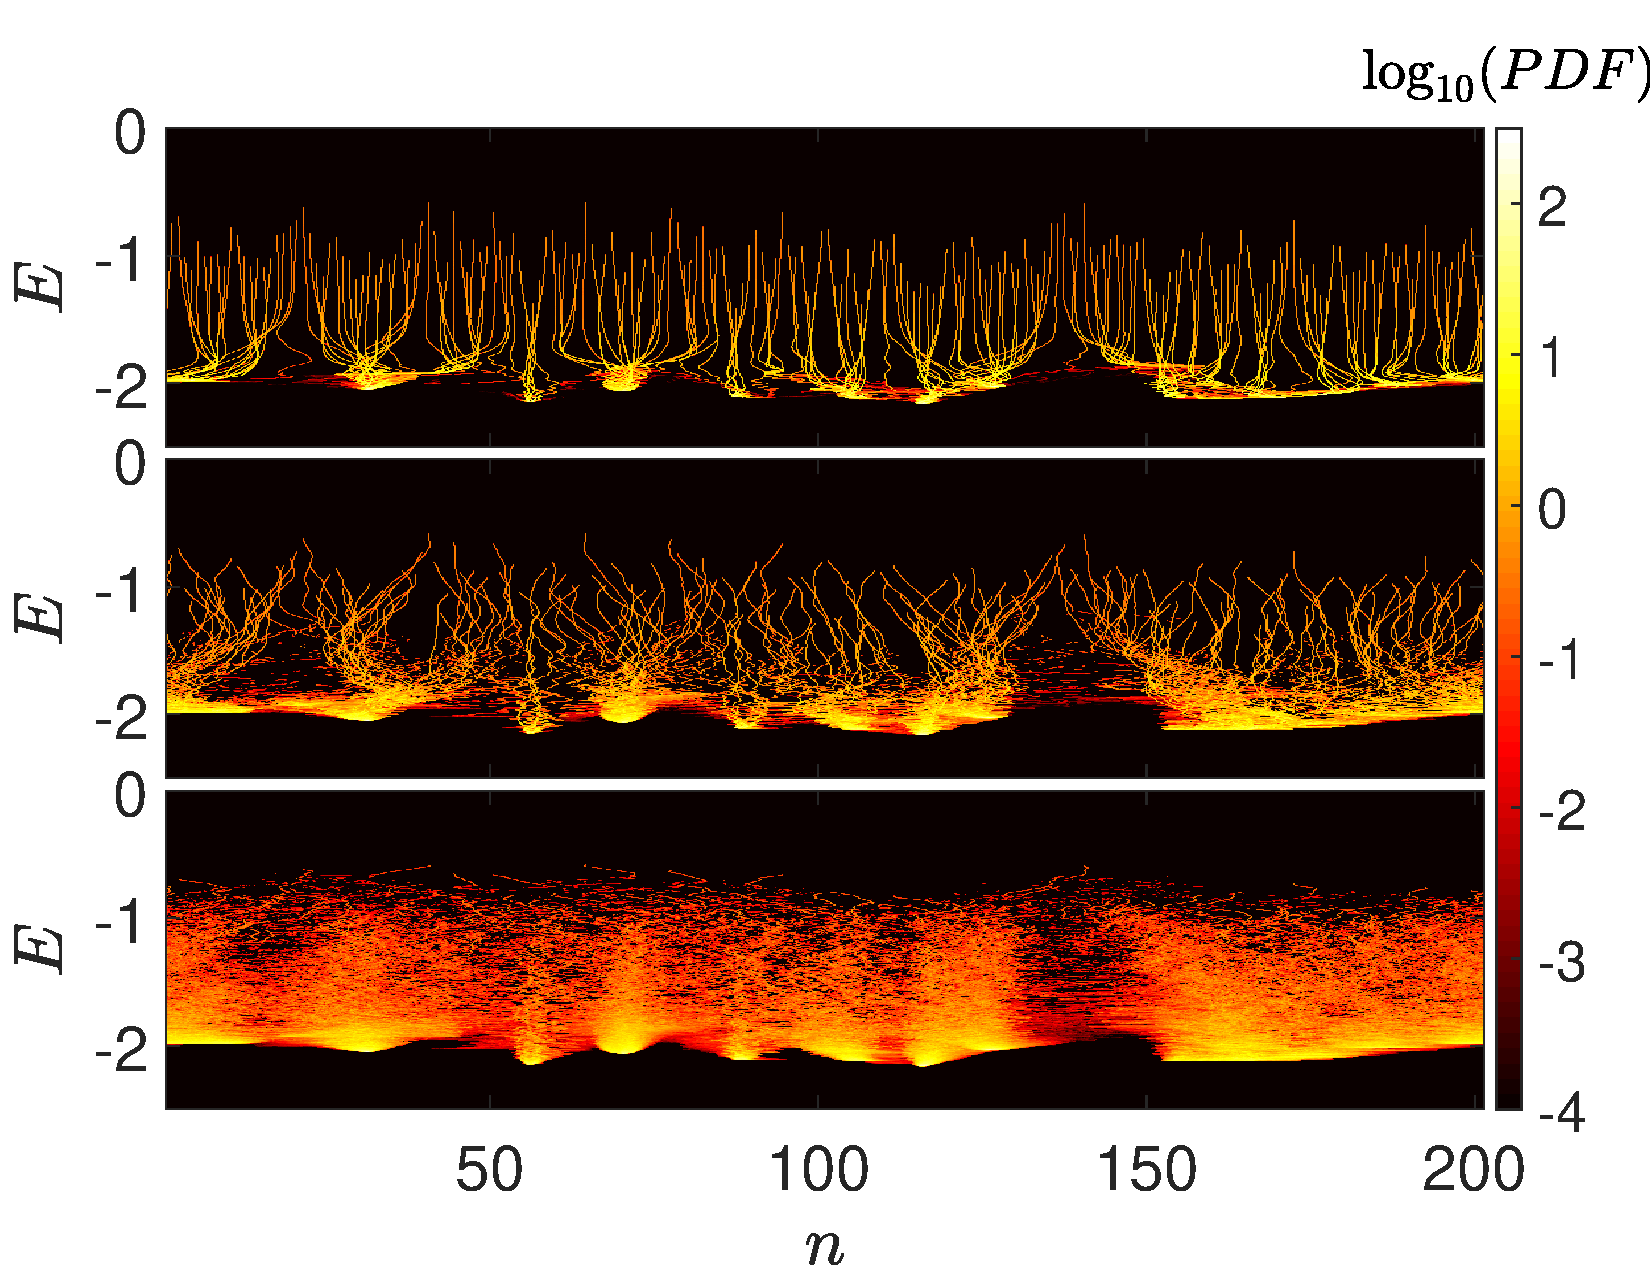
\includegraphics[width=0.5\linewidth]{anderson_prb_1_1}}
		\hfill
		\subcaptionbox{\label{fig:anderson_prb_1_2}}{%
			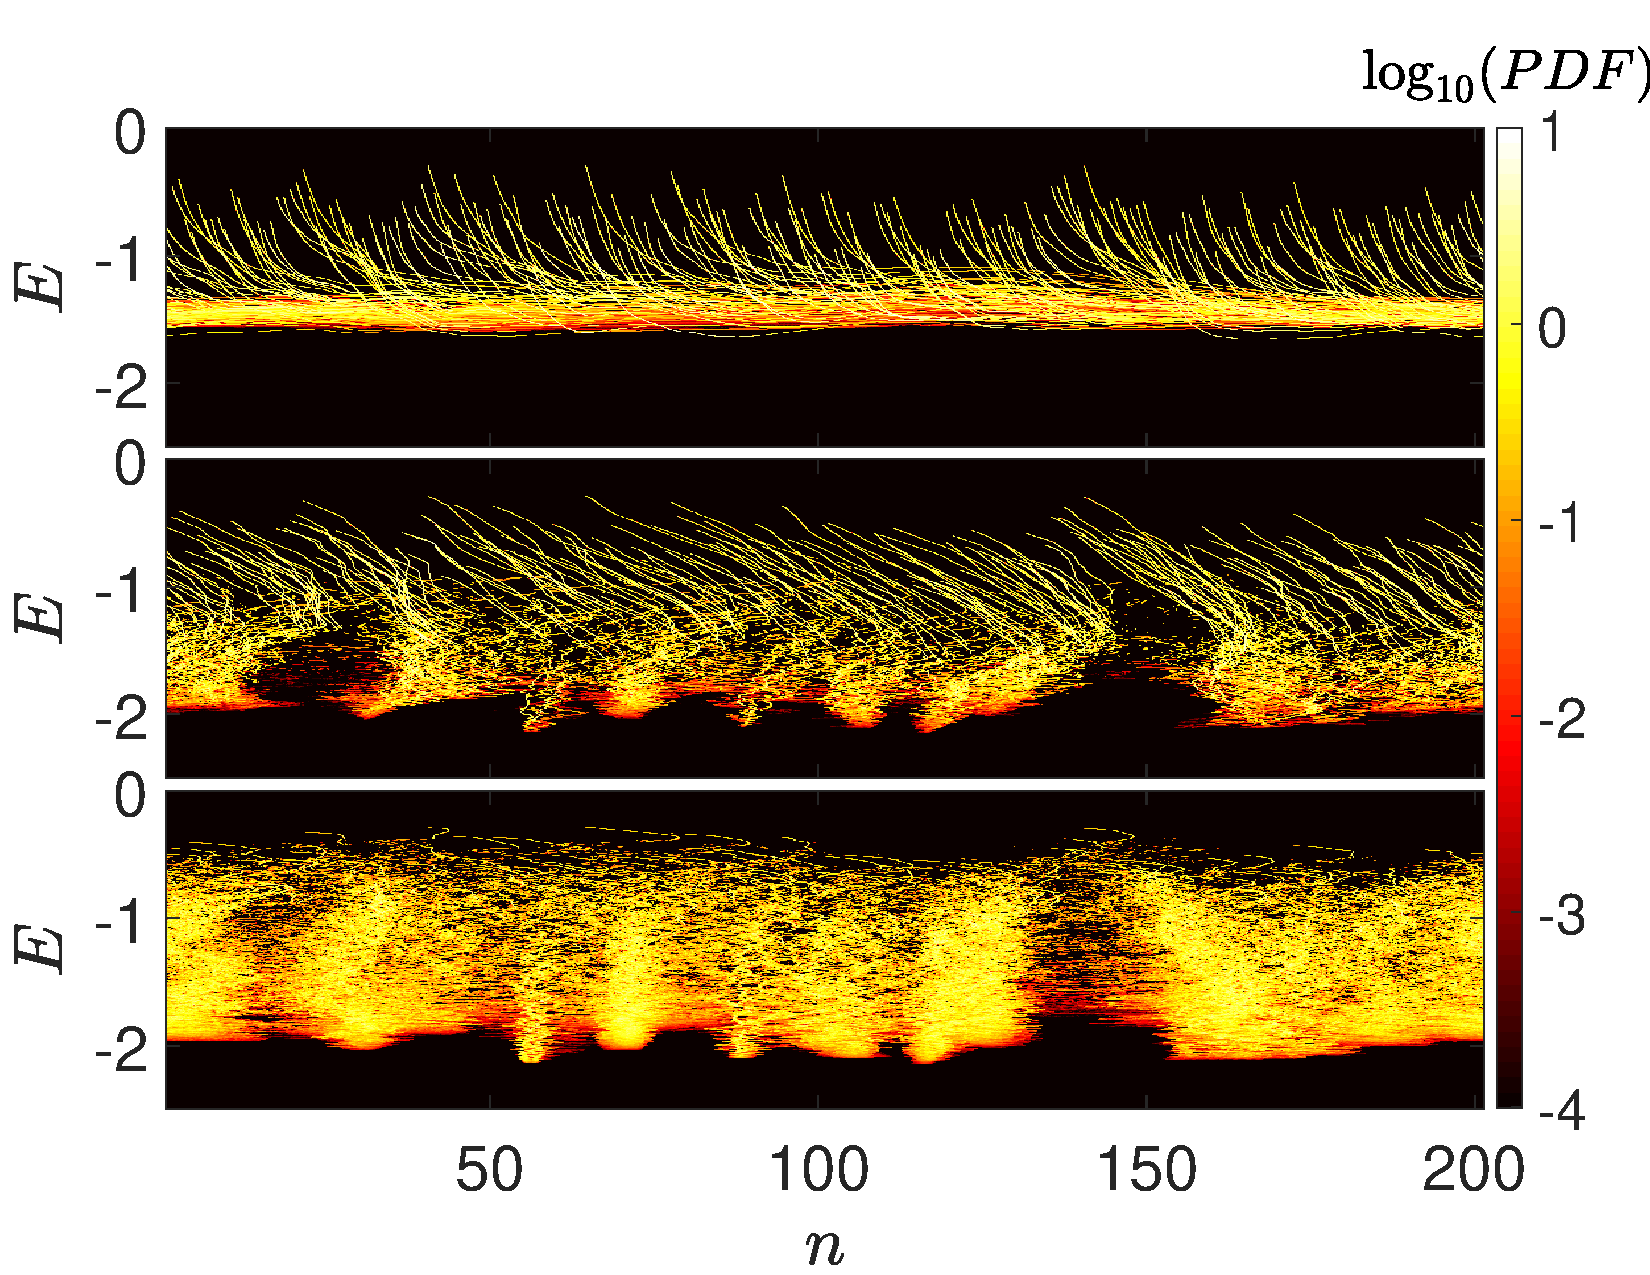
\includegraphics[width=0.5\linewidth]{anderson_prb_1_2}}
		\vfill
		\subcaptionbox[List-of-Figures entry]{\label{fig:anderson_prb_1_3}}{%
			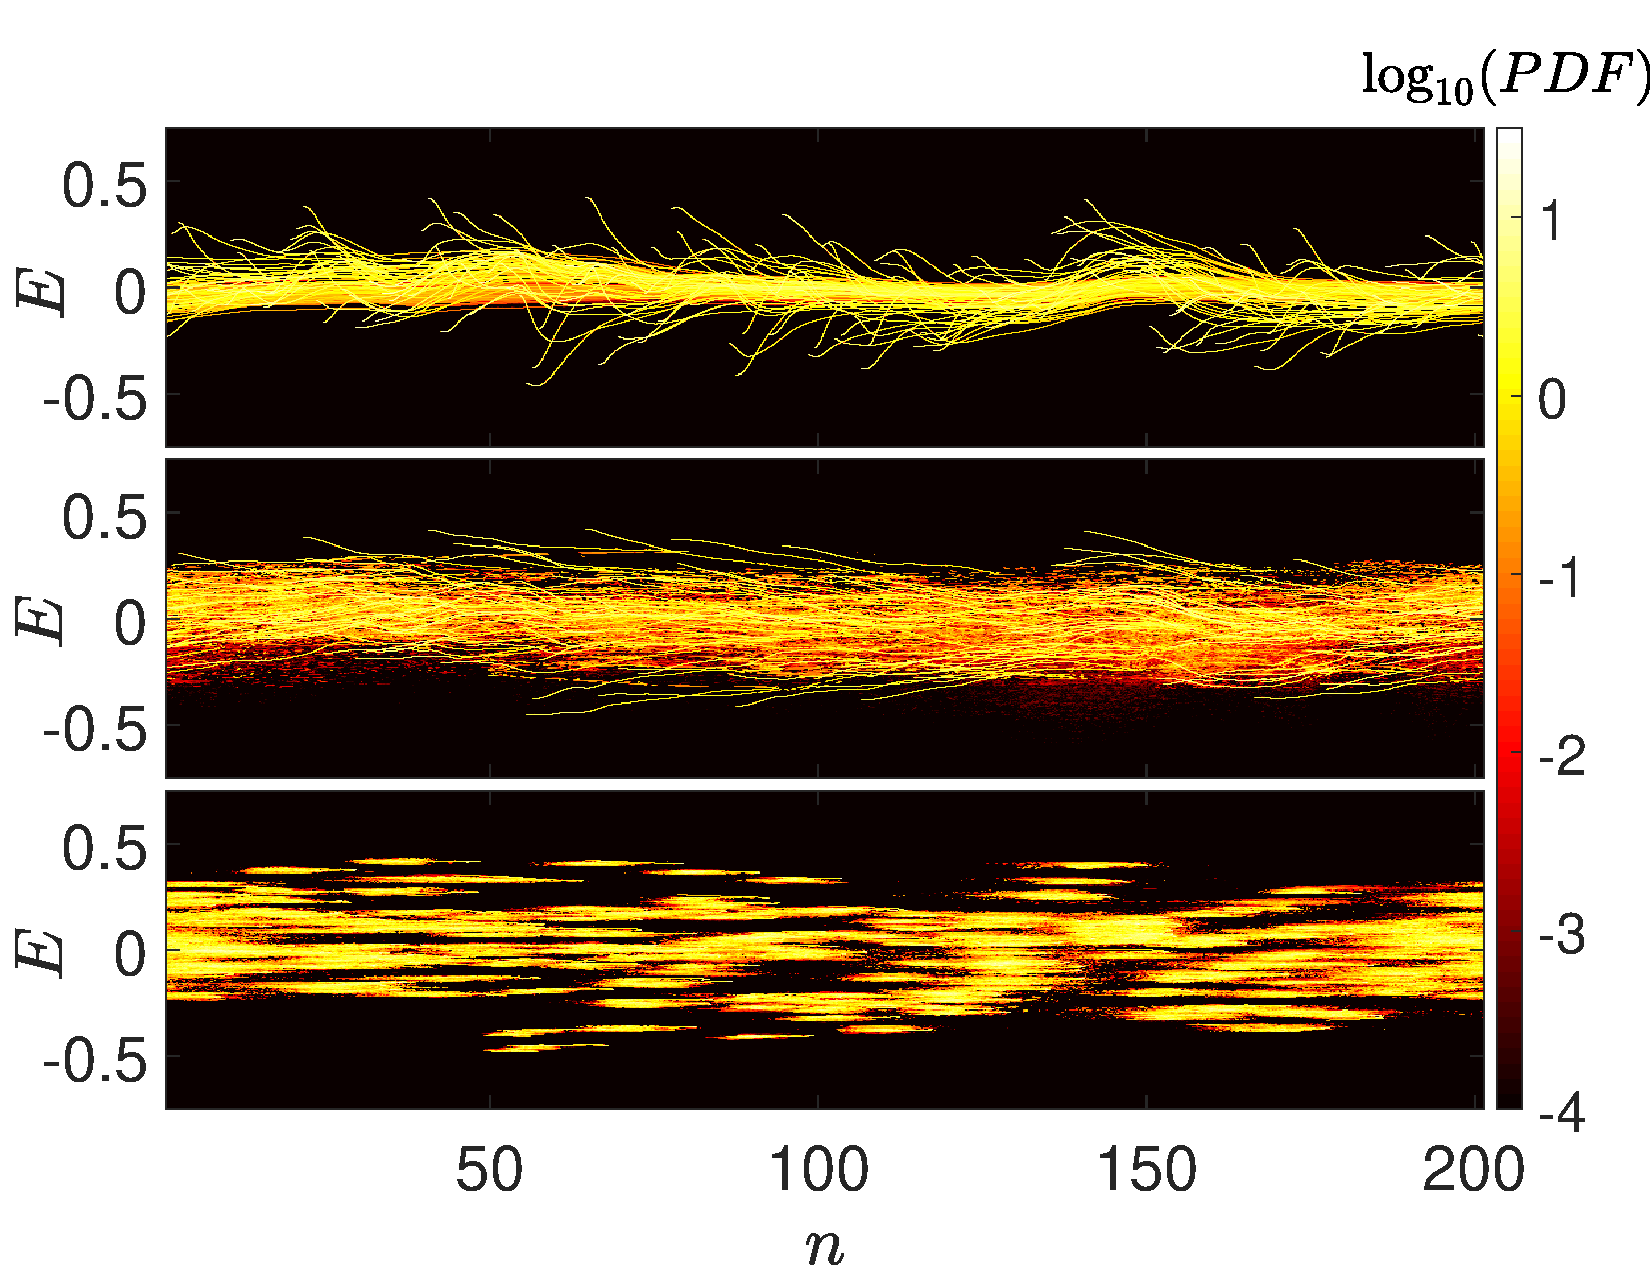
\includegraphics[width=0.5\linewidth]{anderson_prb_1_3}}
		\hfill
		\subcaptionbox{\label{fig:anderson_prb_1_4}}{%
			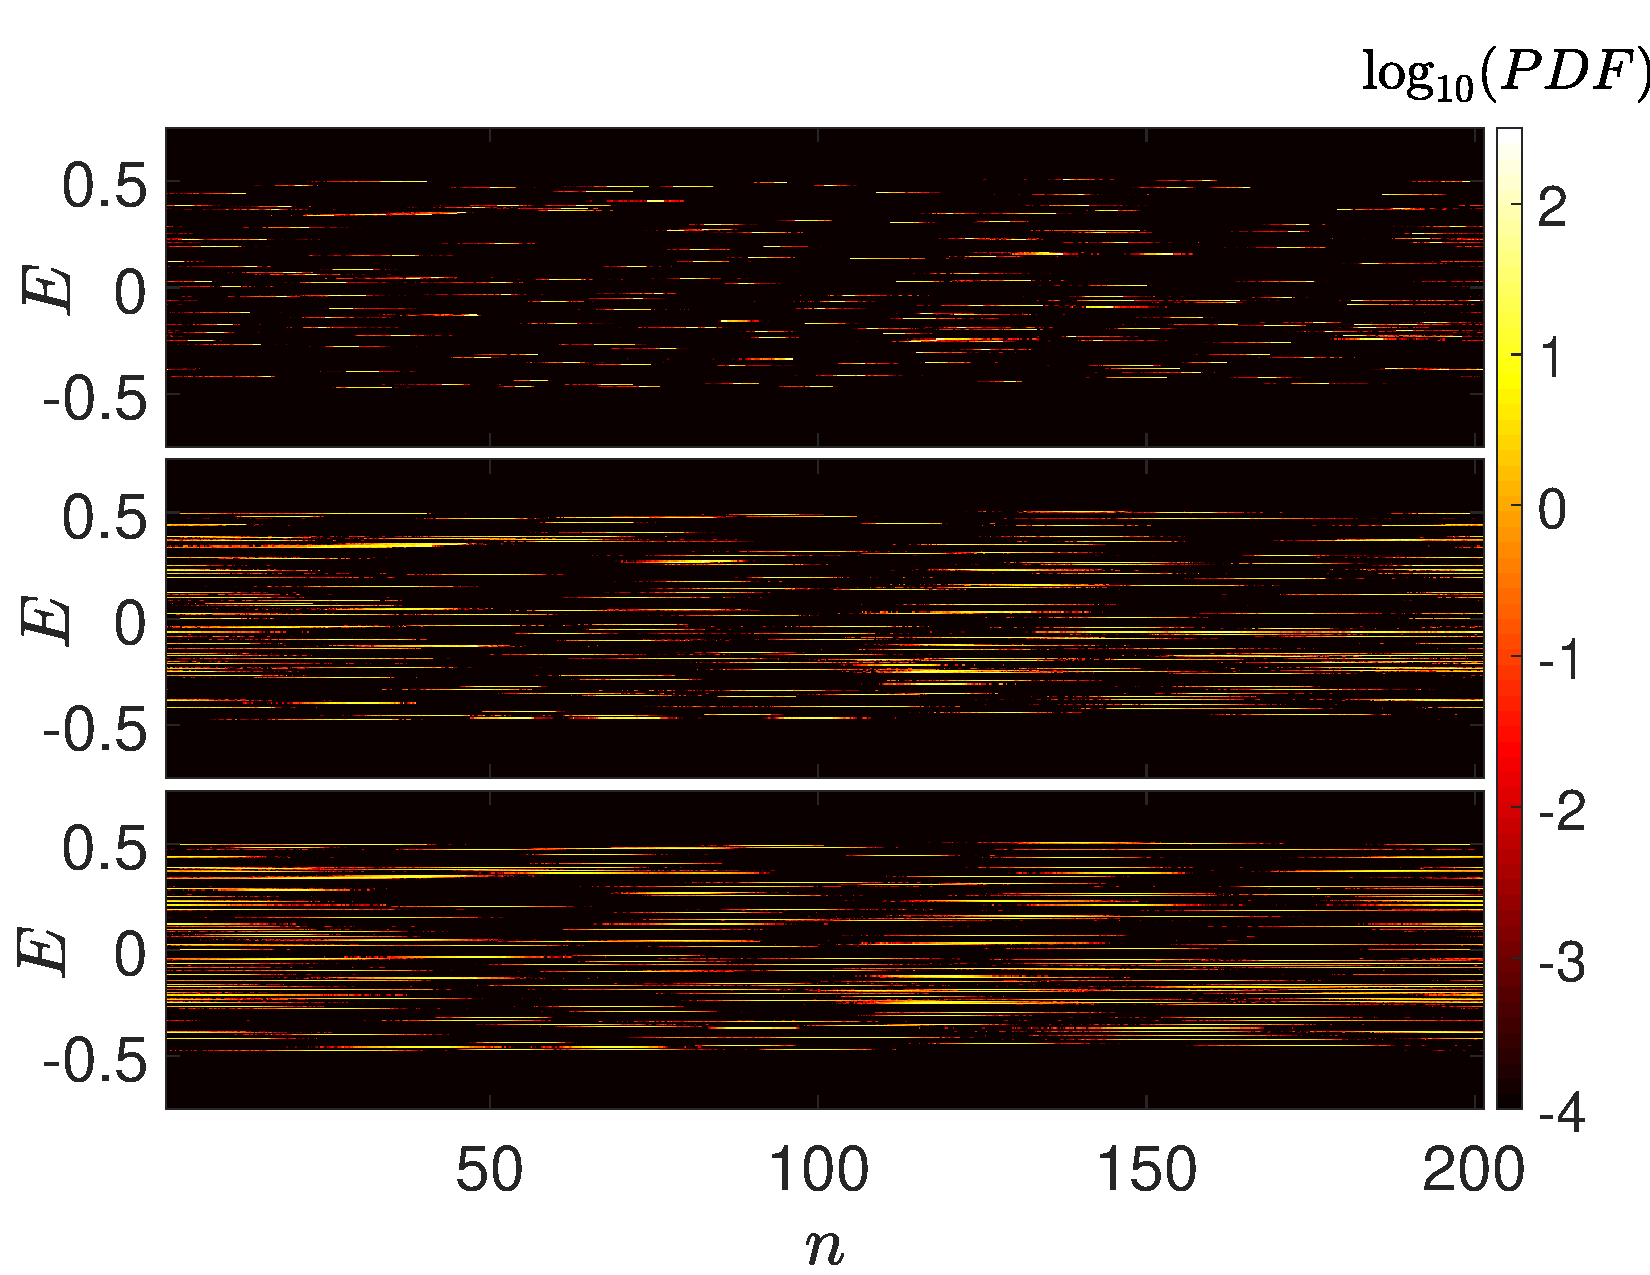
\includegraphics[width=0.5\linewidth]{anderson_prb_1_4}}
	}
	\legend{}
	\caption[Плотность вероятностей квантовых траекторий на плоскости позиции и энергий в зависимости от параметров и скорости неэрмитовой диссипации]
	{
		Функция распределения плотности вероятностей (PDF) квантовых траекторий на плоскости позиции \(n(t)\) и энергии \(E(t))\) для \(\gamma=0.1\) (верхняя часть),  \(\gamma=0.01\) (центральная часть),  \(\gamma=0.001\) (нижняя часть). Результаты для неэрмитовых диссипаторов \cref{eq:anderson_diss_local} "--- (а): \(\alpha=0\); (б): \(\alpha=\frac{\pi}{4}\); (в): \(\alpha=\frac{\pi}{2}\). Дефазирующая диссипация "--- (г).
	}
	\label{fig:anderson_prb_1}
\end{figure}

Изучим структуру асимптотических состояний в виде двумерной функции плотности вероятностей нахождения траекторий на плоскости позиции \(n(t)\) \cref{eq:anderson_position} и энергии \(E(t)\) \cref{eq:anderson_energy} в зависимости от скорости диссипации \(\gamma\). На рисунке \cref{fig:anderson_prb_1} представлена типичная картина для фиксированной реализации беспорядка. 
При \(\alpha=0\) траектории стягиваются вокруг центров локализации, соединённых паутиной переходов. 
Сходимость к центрам локализации и их компактность ослабевают с увеличением скорости диссипации (рисунок \cref{fig:anderson_prb_1_1}, сверху вниз).
Ненулевое значение фазы неэрмитовых диссипаторов \(\alpha=\frac{\pi}{4}\) приводит к сильному перекосу траекторий (рисунок \cref{fig:anderson_prb_1_2}). 
В конечном итоге, при \(\alpha=\frac{\pi}{2}\), центры локализации становятся плохо различимыми (рисунок \cref{fig:anderson_prb_1_3}). 
Следует отметить, что локализация энергии сохраняется, изменяясь от нижней границы спектра собственных чисел модели Андерсона \cref{eq:anderson_evals} при \(\alpha=0\) к середине спектра при \(\alpha=\frac{\pi}{2}\). 
Совсем иначе выглядит картина для случая дефазируюшей диссипации \cref{eq:anderson_diss_dephase}, при котором распределение плотности вероятности является случайным и охватывает весь спектр собственных значений модели Андерсона \cref{eq:anderson_evals} (рисунок \cref{fig:anderson_prb_1_4}).

\begin{figure}[ht]
	\centerfloat{
		\hfill
		\subcaptionbox[List-of-Figures entry]{\label{fig:anderson_prb_2_1}}{%
			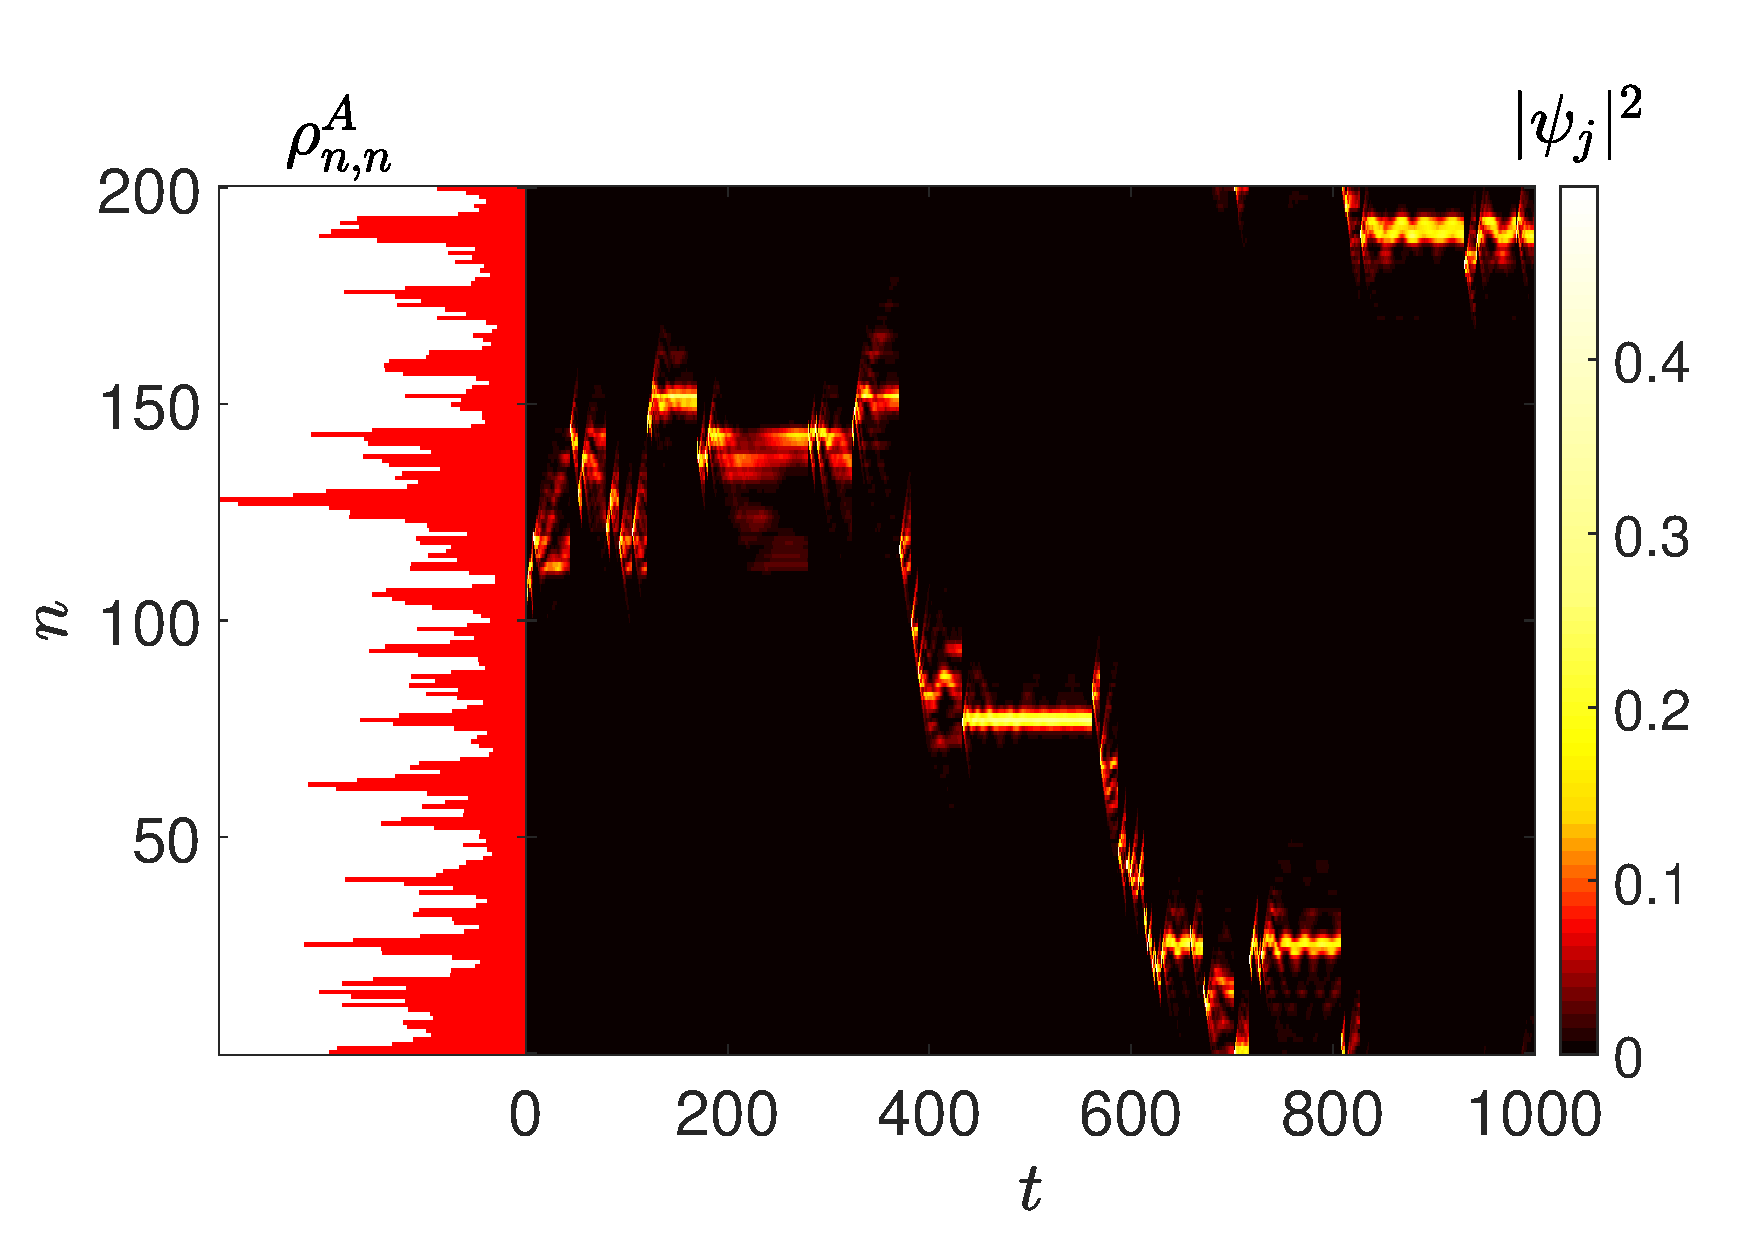
\includegraphics[width=0.5\linewidth]{anderson_prb_2_1}}
		\hfill
		\subcaptionbox{\label{fig:anderson_prb_2_2}}{%
			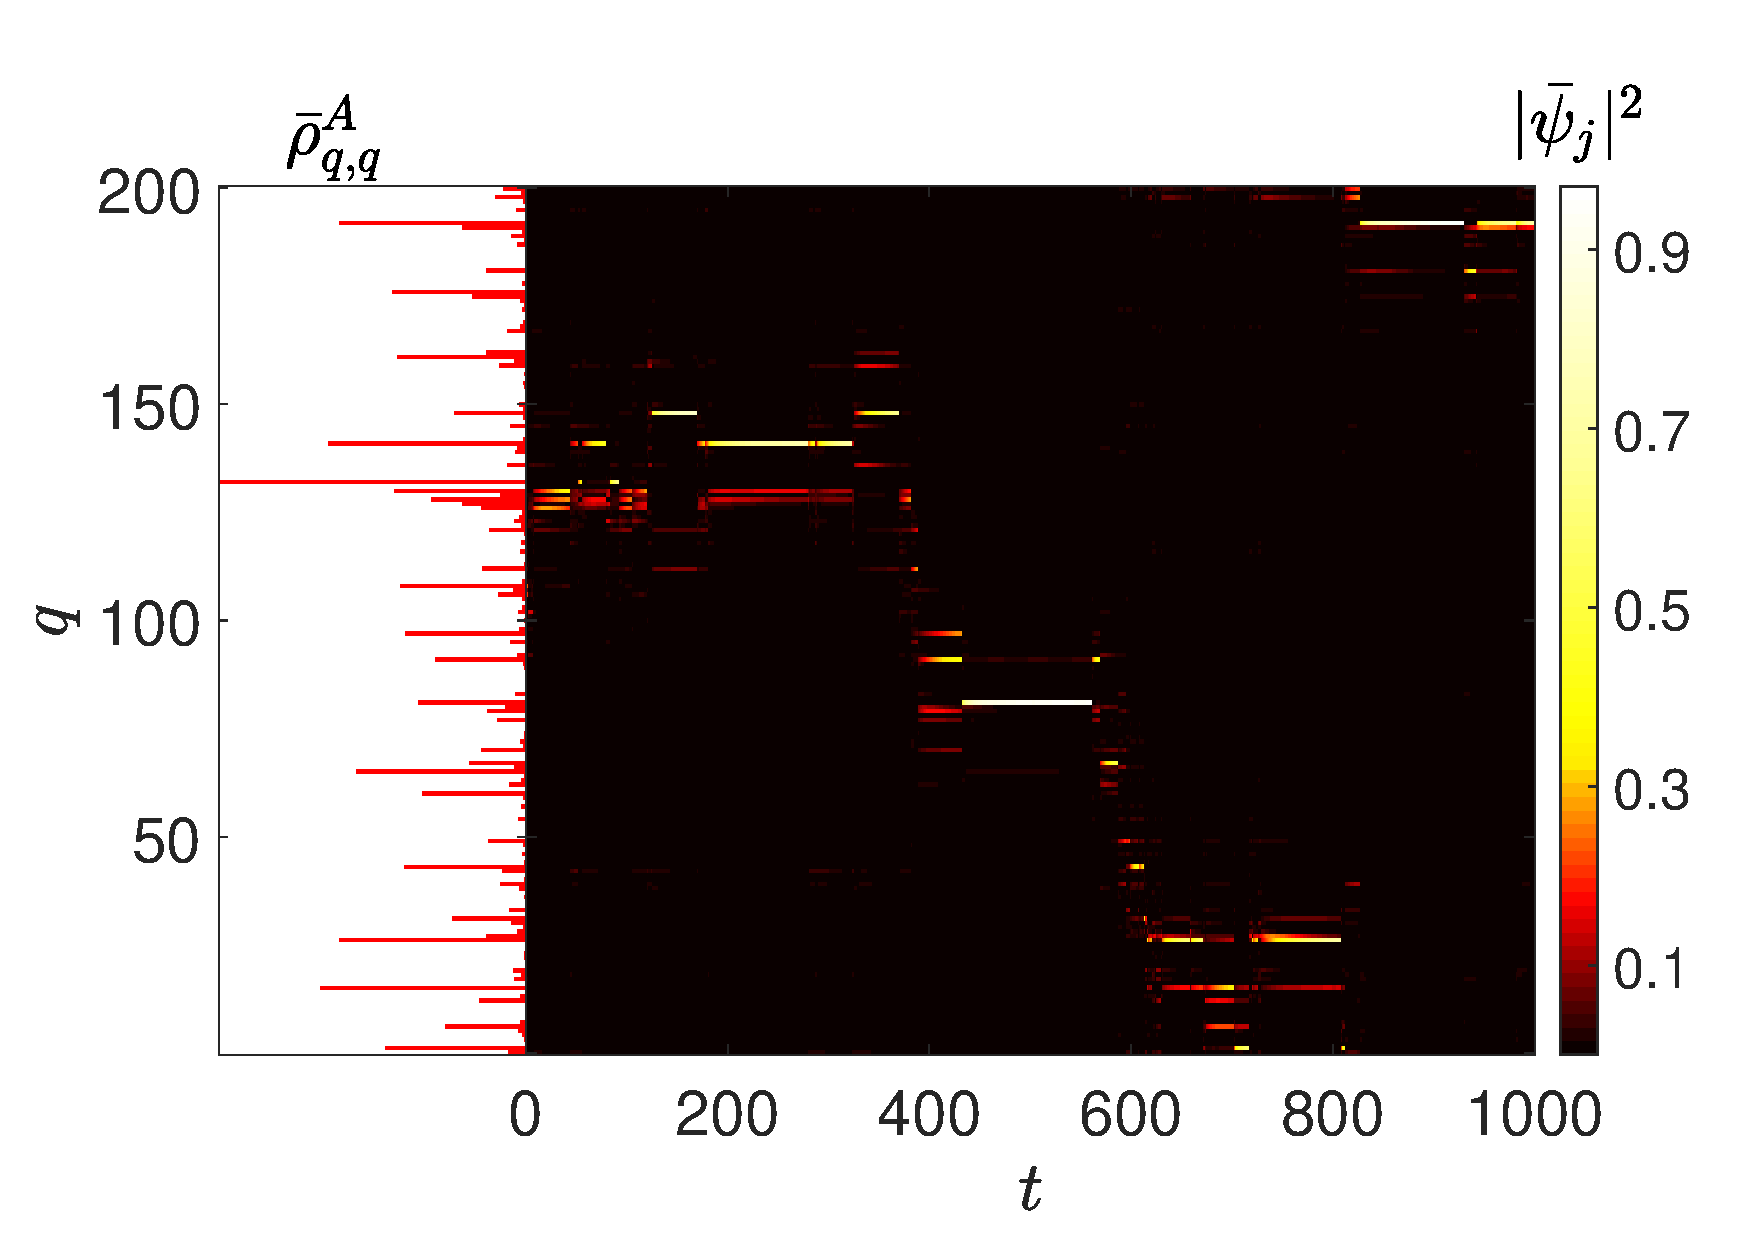
\includegraphics[width=0.5\linewidth]{anderson_prb_2_2}}
		\vfill
		\subcaptionbox[List-of-Figures entry]{\label{fig:anderson_prb_2_3}}{%
			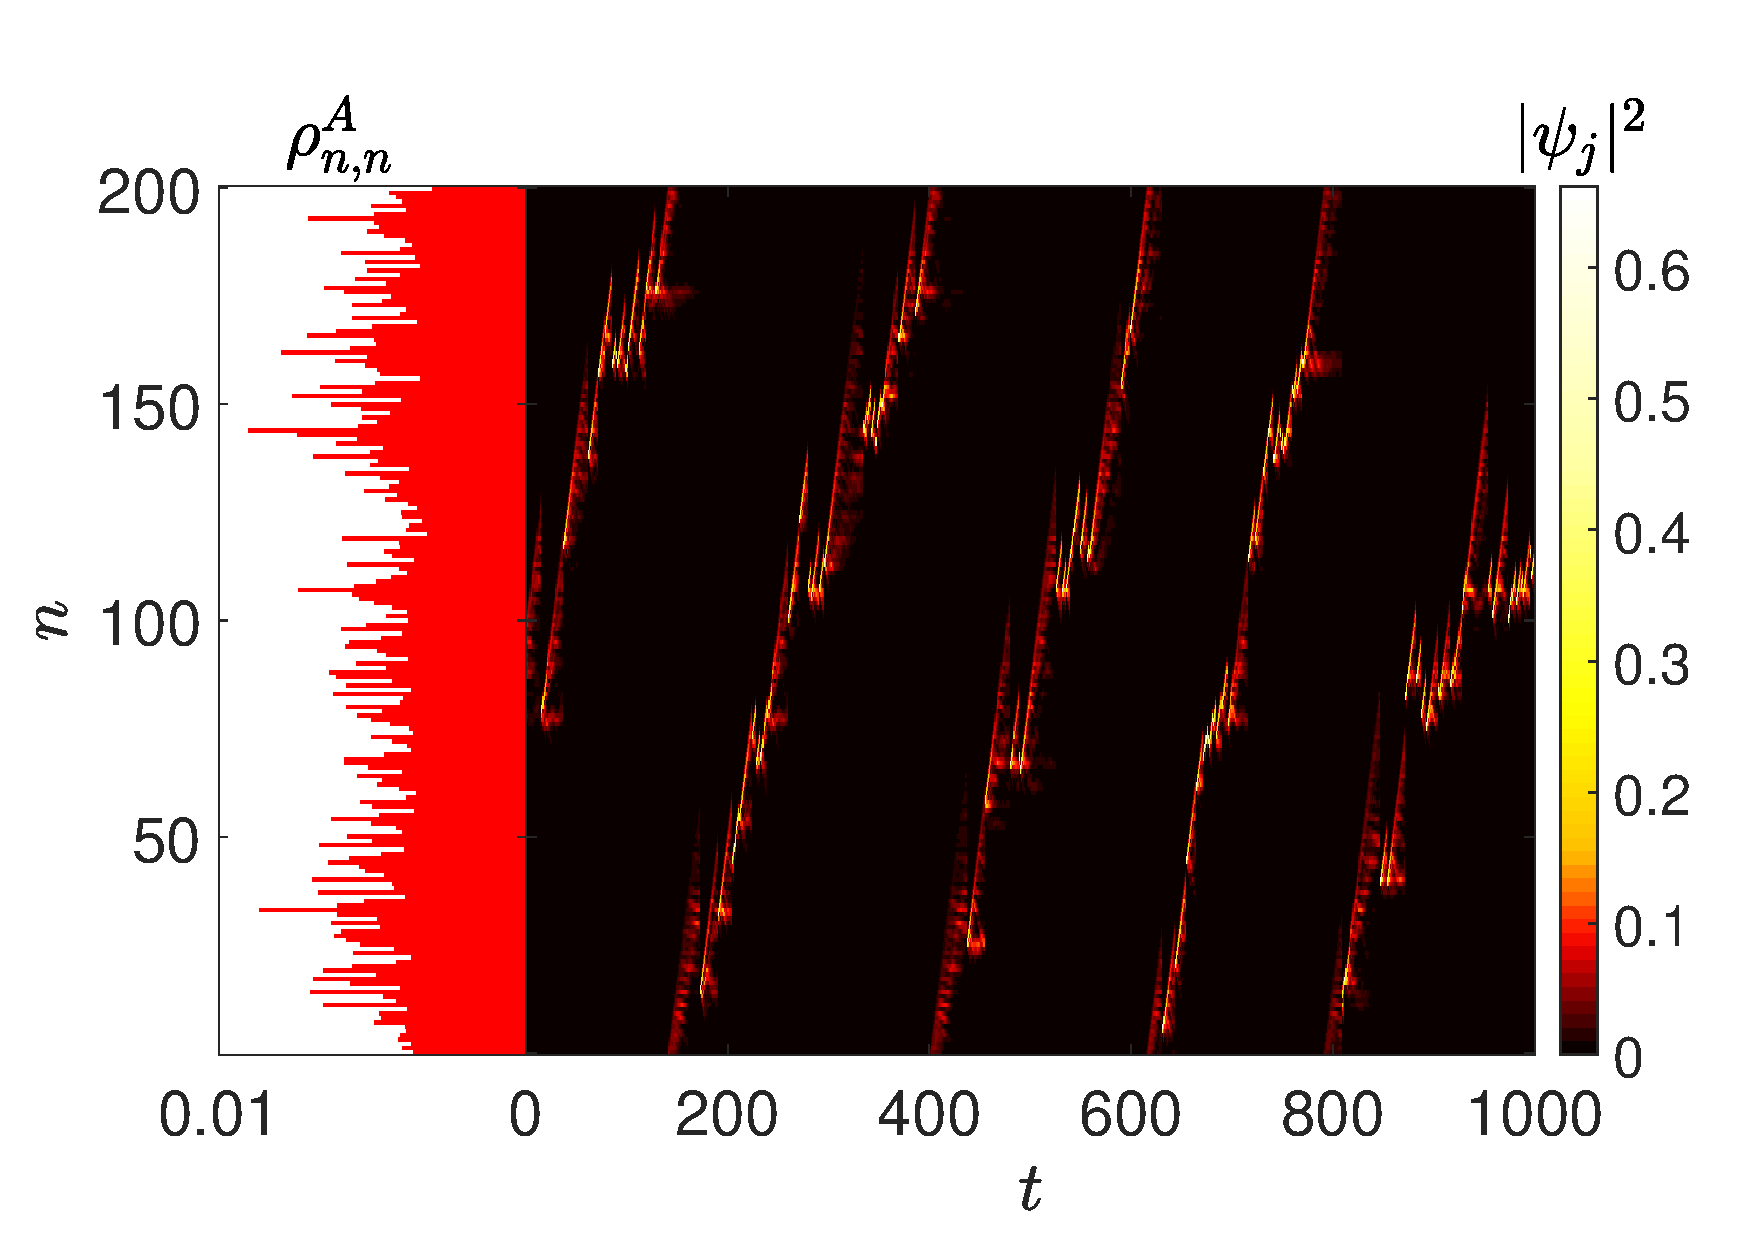
\includegraphics[width=0.5\linewidth]{anderson_prb_2_3}}
		\hfill
		\subcaptionbox{\label{fig:anderson_prb_2_4}}{%
			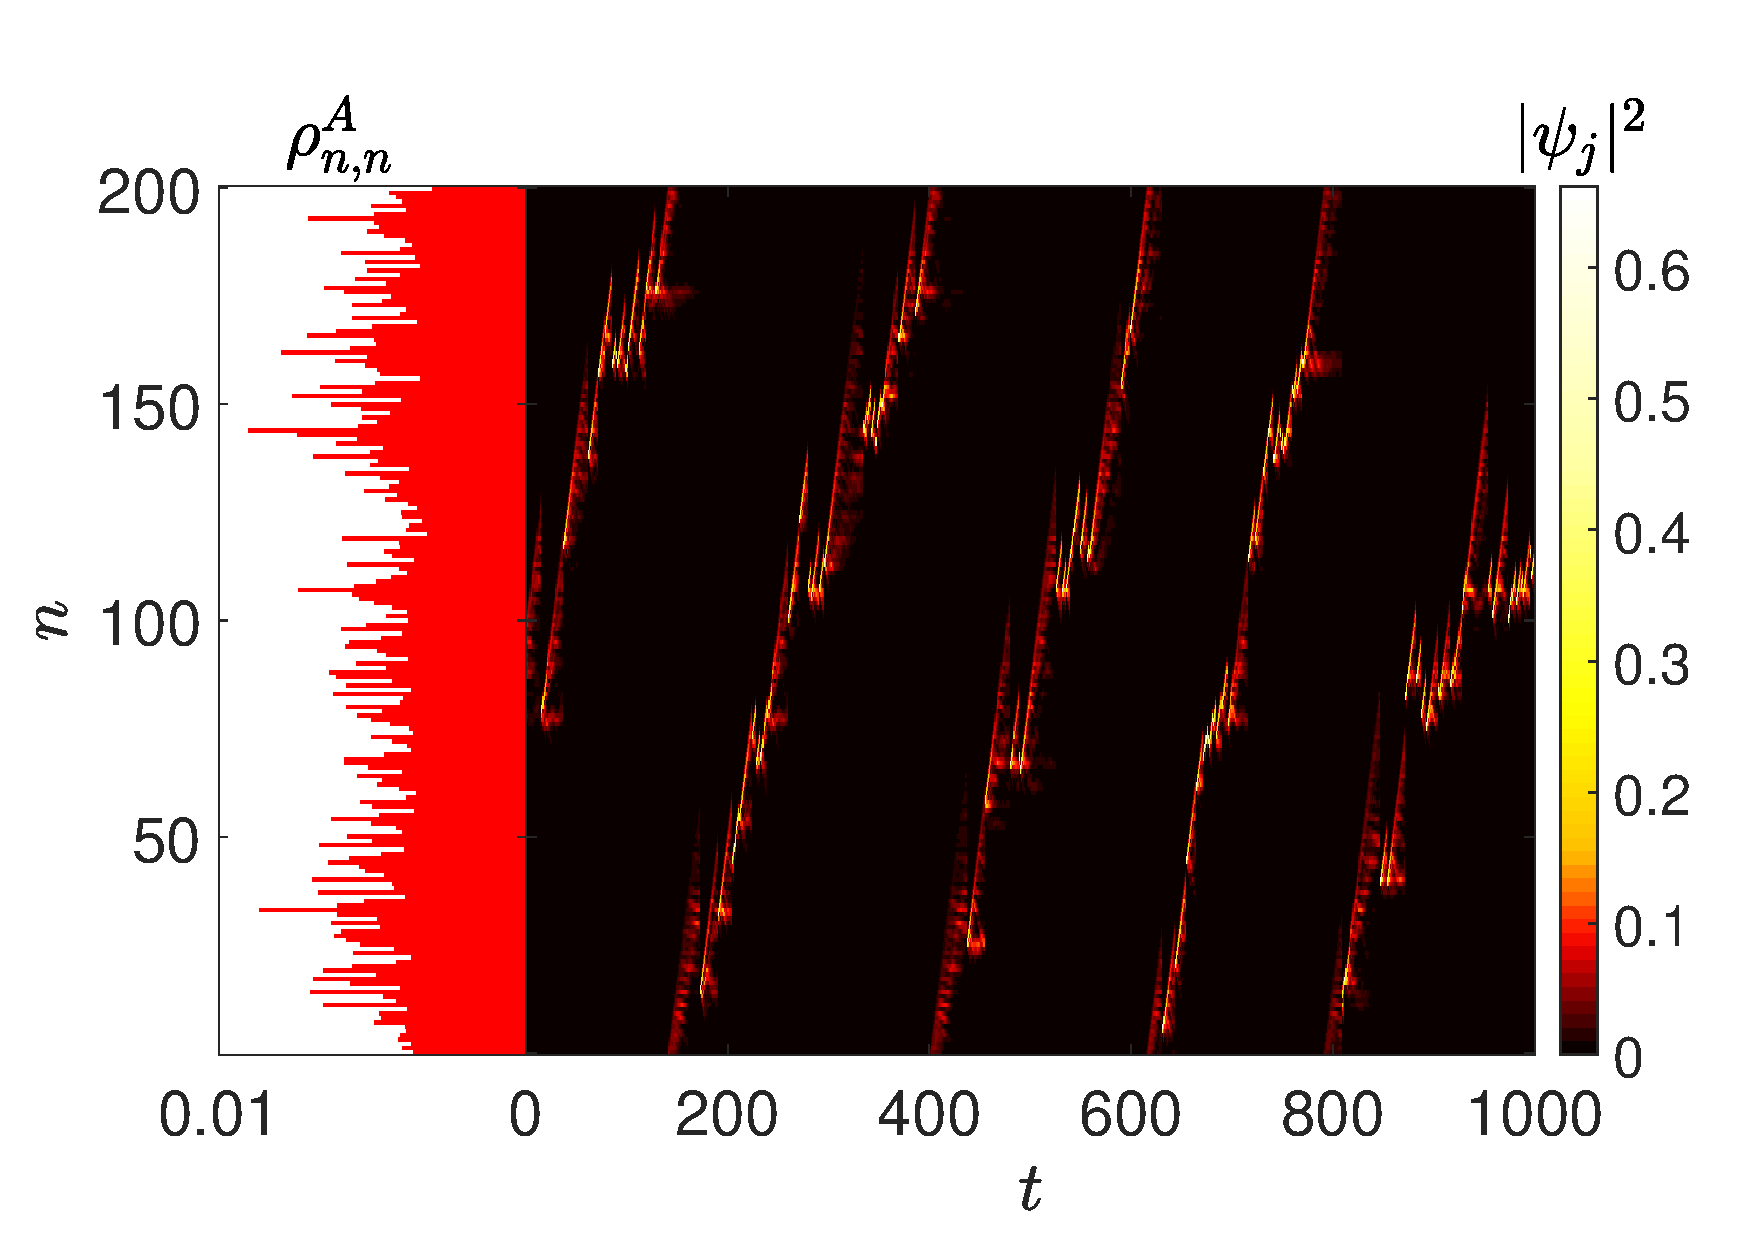
\includegraphics[width=0.5\linewidth]{anderson_prb_2_4}}
	}
	\legend{}
	\caption[Динамика квантовых траекторий на квантовых аттракторах в зависимости от параметров неэрмитовой диссипации]
	{
		Диагональные элементы асимптотической матрицы плотности (на левых вставках) и эволюция на аттракторе квадрата волновой функции отдельно взятой квантовой траектории (основные части на рисунках). (a): \(\alpha = 0\), в исходном базисе; (б): \(\alpha = 0\), в базисе Андерсоновских мод, отсортированных по позиции \(n\) \cref{eq:anderson_position}; (в): \(\alpha=\frac{\pi}{4}\), в исходном базисе; (г): дефазирующая диссипация \cref{eq:anderson_diss_dephase}. 
	}
	\label{fig:anderson_prb_2}
\end{figure}

Исследуем теперь динамику волновых функций \(\psi_j(t)\) единичных квантовых траекторий (раздел \cref{sec:ch1/qj}), которые эволюционируют с неэрмитовым гамитонианом \cref{eq:H_nonhermit}, в сопоставлении с асимптотическим состоянием \(\rho^A\) (или \(\bar{\rho}^A\) "--- в базисе собственных состояний модели Андерсона \cref{eq:anderson_rho_in_eigen_basis}). 
В случае нулевой фазы \(\alpha=0\) наблюдается прерывистая динамика состоящая из длительных циркуляций возле центров локализации и быстрых переходов между ними (рисунок \cref{fig:anderson_prb_2_1}). 
Если данную волновую функцию перевести в базис собственных состояний модели Андерсона,  отсортированных по позиции \(n\) \cref{eq:anderson_position}, то можно заметить, что циркуляции происходят на модах Андерсона, которые формируют асимптотическое состояние равновесия \cite{Yusipov2017} (рисунок \cref{fig:anderson_prb_2_2}). 
Если рассмотреть ненулевую фазу неэрмитовых диссипаторов, то динамика резко изменится: для \(\alpha=\frac{\pi}{4}\) незначительные циркуляции возле центов локализации сохраняются, но самый существенный вклад в динамику вносит баллистическое распространение волновых пакетов (рисунок \cref{fig:anderson_prb_2_3}). 
Дефазирующая диссипация не несёт какой-либо пространственно-временной структуры (рисунок \cref{fig:anderson_prb_2_4}).

\begin{figure}[h]
	\centerfloat{
		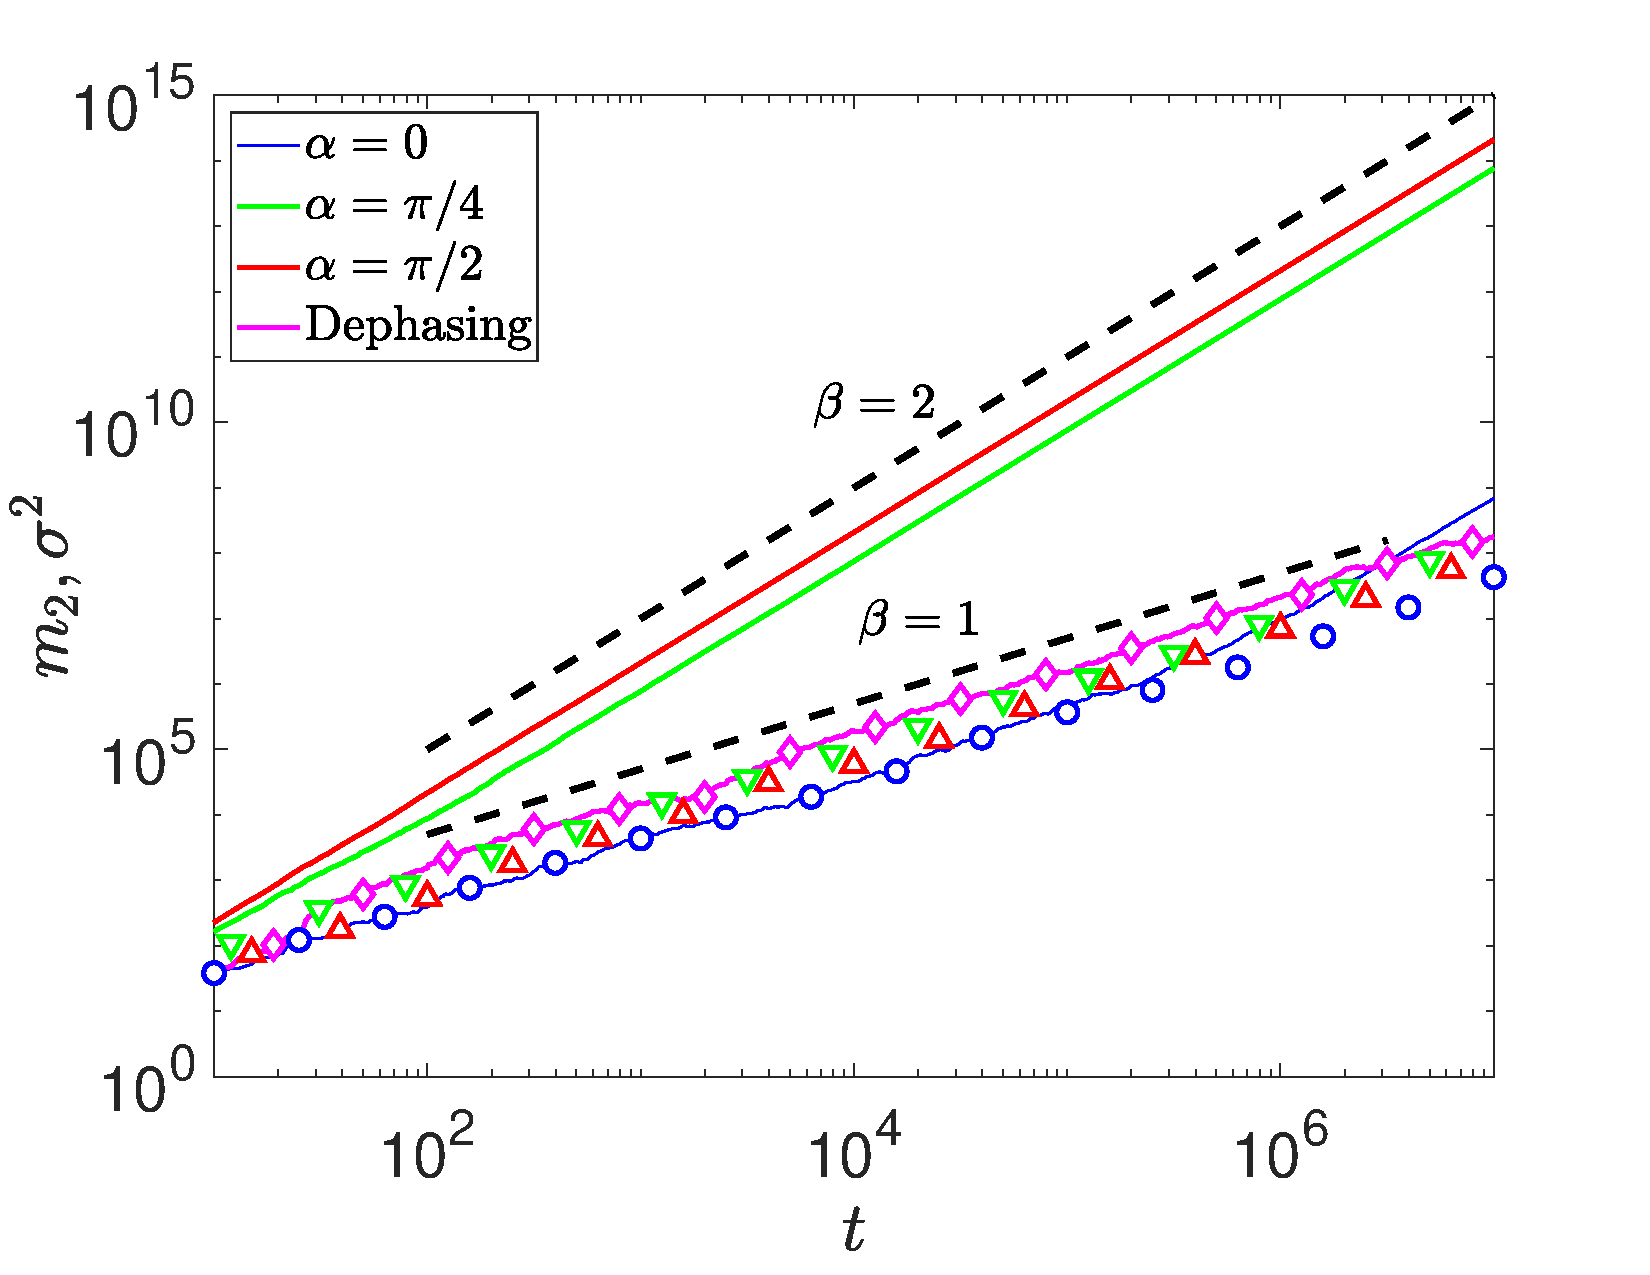
\includegraphics[scale=0.55]{anderson_prb_3}
	}
	\caption[Характеристика динамики квантовых траекторий на квантовых аттракторах]{
		Эволюция второго момента смещения \(m_2(t)\) (сплошные линии) и квадрата отклонения от баллистического распространения волновых пакетов \(\sigma_2(t)\) (символы) для разных типов диссипации в открытой модели Андерсона.
	}
	\label{fig:anderson_prb_3}
\end{figure}

Для количественной оценки распространения волнового пакета отдельно взятой квантовой траектории используются следующие характеристики, усреднённые по ансамблю траекторий: второй момент смещения \(m_2(t)\), средняя скорость \(v\) и квадрат отклонения от баллистического распространения волновых пакетов \(\sigma_2(t)\). Данные характеристики выражаются при помощи следующих соотношений:
\begin{equation}
	\label{eq:anderson_m2}
	\begin{gathered}
		m_2(t) = \frac{1}{M_r} \sum_{j=1}^{M_r} \left( n_j(t) - n_j(t^A) \right)^2,
	\end{gathered}
\end{equation}
\begin{equation}
	\label{eq:anderson_velocity}
	\begin{gathered}
		v = \frac{1}{M_r} \sum_{j=1}^{M_r} \frac{n_j(t^A + t^O) - n_j(t^A)}{t^O},
	\end{gathered}
\end{equation}
\begin{equation}
	\label{eq:anderson_sigma_2}
	\begin{gathered}
		\sigma_2(t) = \frac{1}{M_r} \sum_{j=1}^{M_r} \left( n_j(t) - n_j(t^A) - v \cdot (t-t^A) \right)^2,
	\end{gathered}
\end{equation}
где \(n_j(t)\) "--- позиция \(j\)-ой траектории \cref{eq:anderson_position}. Стоит отметить, что во всех случаях эволюция второго момента смещения \cref{eq:anderson_m2} от времени является степенным законом с разным показателем степени \(\beta\):
\begin{equation}
	\label{eq:anderson_m2_fit}
	\begin{gathered}
		m_2(t) \approx t^\beta .
	\end{gathered}
\end{equation}
Для неэрмитовых диссипаторов с фазой \(\alpha=0\), а также дефазирующей диссипации имеет место режим нормальной диффузии (\(\beta \approx 1\)), в то время как ля \(\alpha=\frac{\pi}{4}\) и \(\alpha=\frac{\pi}{2}\) наблюдается баллистическое распространение волновых пакетов с \(\beta \approx 2\) (рисунок \cref{fig:anderson_prb_3}, сплошные линии). В то же время квадрат отклонения от баллистического распространения волновых пакетов \cref{eq:anderson_sigma_2} демонстрирует сопутствующую диффузию: \(\sigma_2(t) \approx t^\beta\), \(\beta=1\) (рисунок \cref{fig:anderson_prb_3}, символы).

\begin{figure}[h]
	\centerfloat{
		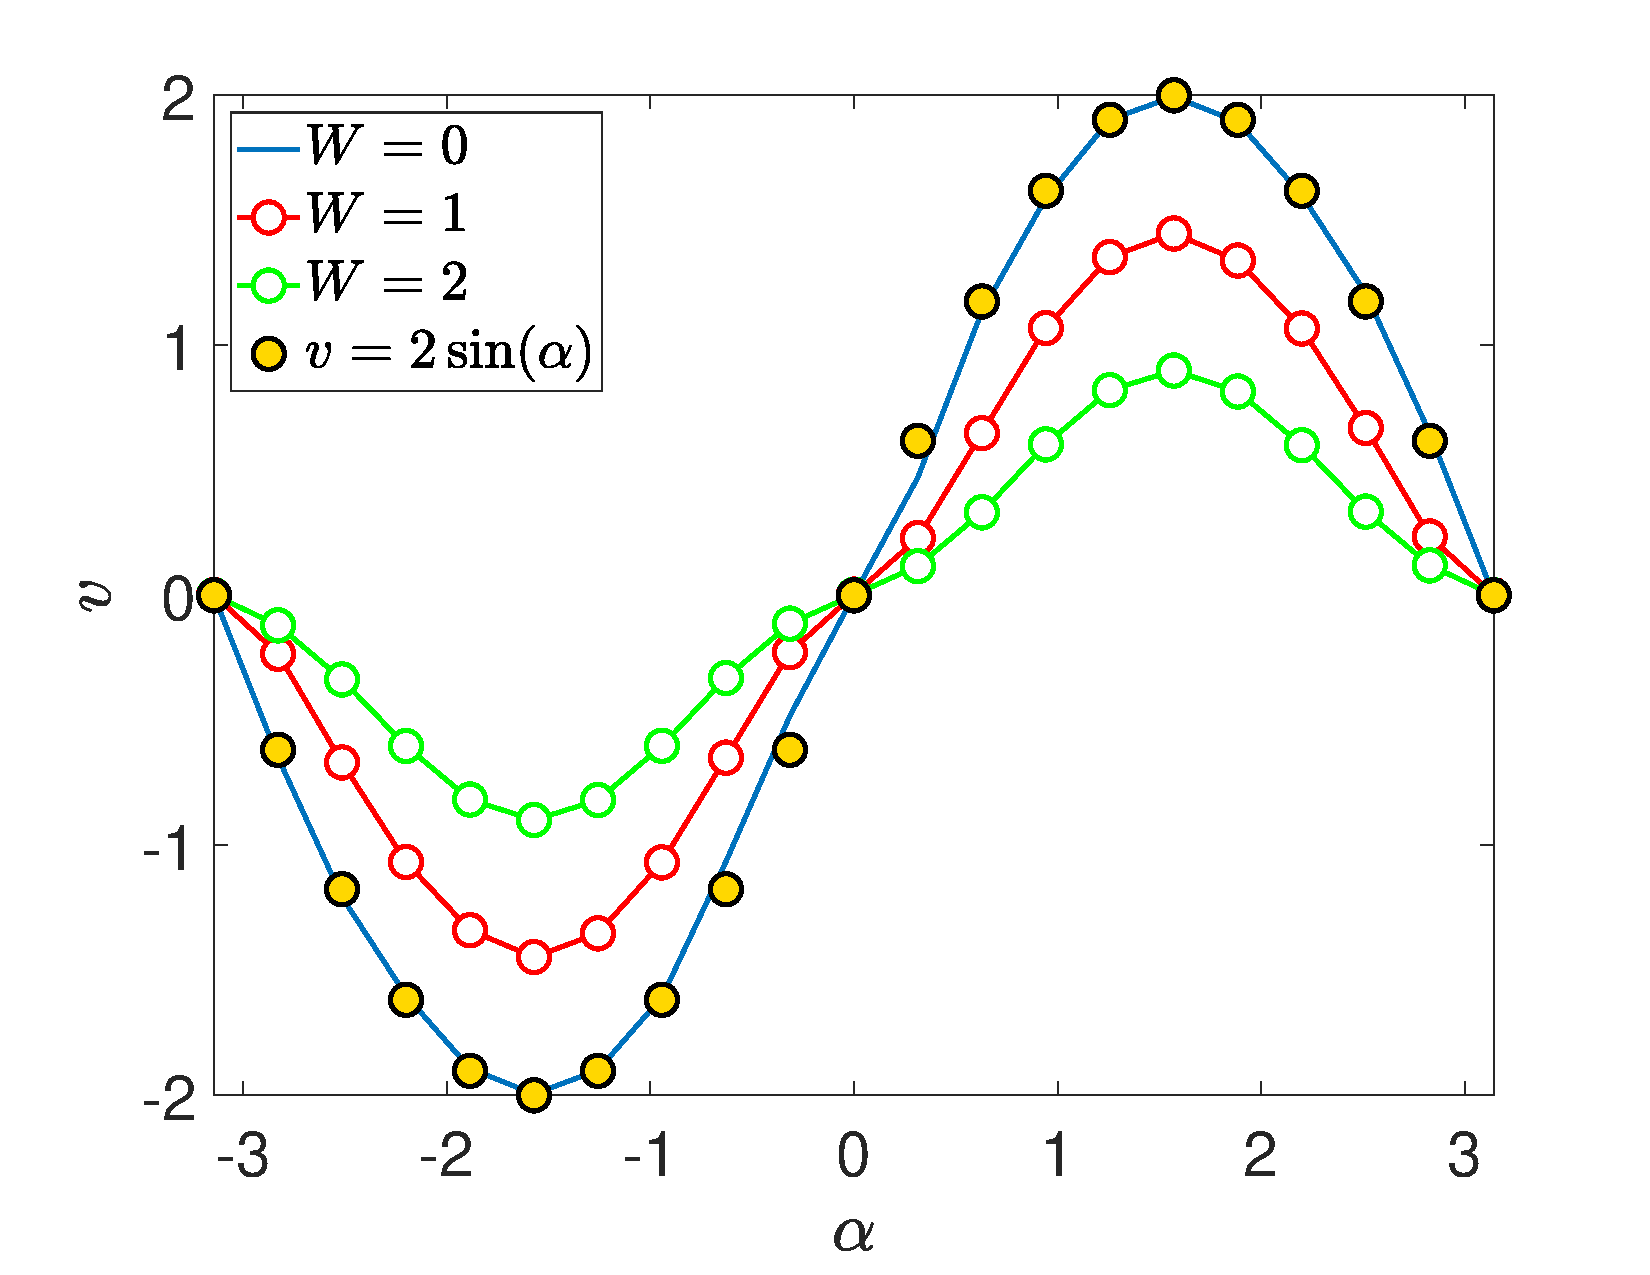
\includegraphics[scale=0.55]{anderson_prb_4}
	}
	\caption[Скорость распространения волновых пакетов в зависимости от параметров неэрмитовой диссипации]{
		Средняя скорость распространения волновых пакетов \cref{eq:anderson_velocity} в зависимости от фазы диссипатора \(\alpha\) при разных значениях пространственного беспорядка \(W\).
	}
	\label{fig:anderson_prb_4}
\end{figure}

Переход от диффузионного к баллистическому распространению при ненулевом \(\alpha\) вызван взаимодействием между беспорядком и диссипацией. 
Как было отмечено в разделе \cref{sec:ch2/epjb}, диссипация отбирает моды Андерсона из определённой части спектра. 
Эти моды заимствуют пространственно-фазовые свойства собственных состояний плоских волн с нулевым беспорядком и волновыми числами близкими к фазе диссипатора (\(k\approx \alpha\)) \cite{Vershinina2017, Ishii1973}. 
Перекрываясь в пространстве, данные экспоненциально локализованные моды взаимодействуют за счёт диссипативной связи, которая обеспечивает направленное распространение квантового волнового пакета с определённой скоростью. 
Данная скорость, в свою очередь, зависит от фазы диссипатора \(\alpha\). 
На рисунке \cref{fig:anderson_prb_4} изображена зависимость средней скорости \cref{eq:anderson_velocity} от параметра фазы неэрмитовых диссипаторов \cref{eq:anderson_diss_local}. В случае отсутствия беспорядка в системе (\(W=0\)) скорость распространения волновых пакетов определяется групповой скоростью плоских волн (тёмных состояний при \(k=\alpha\)):
\begin{equation}
	\label{eq:anderson_velocity_sin}
	\begin{gathered}
		v(\alpha) = v_{group}(k)|_{k=\alpha} = 2 \sin(\alpha) .
	\end{gathered}
\end{equation}
Синей сплошной линией на рисунке \cref{fig:anderson_prb_4} показан численный результат для системы без беспорядка, жёлтые символы "--- теоретическая оценка \(2 \sin(\alpha)\). 
При введении беспорядка в систему, синусоидальная зависимость сохраняется, но амплитуда уменьшается (красная и зелёная линии на рисунке \cref{fig:anderson_prb_4}).

\begin{figure}[h]
	\centerfloat{
		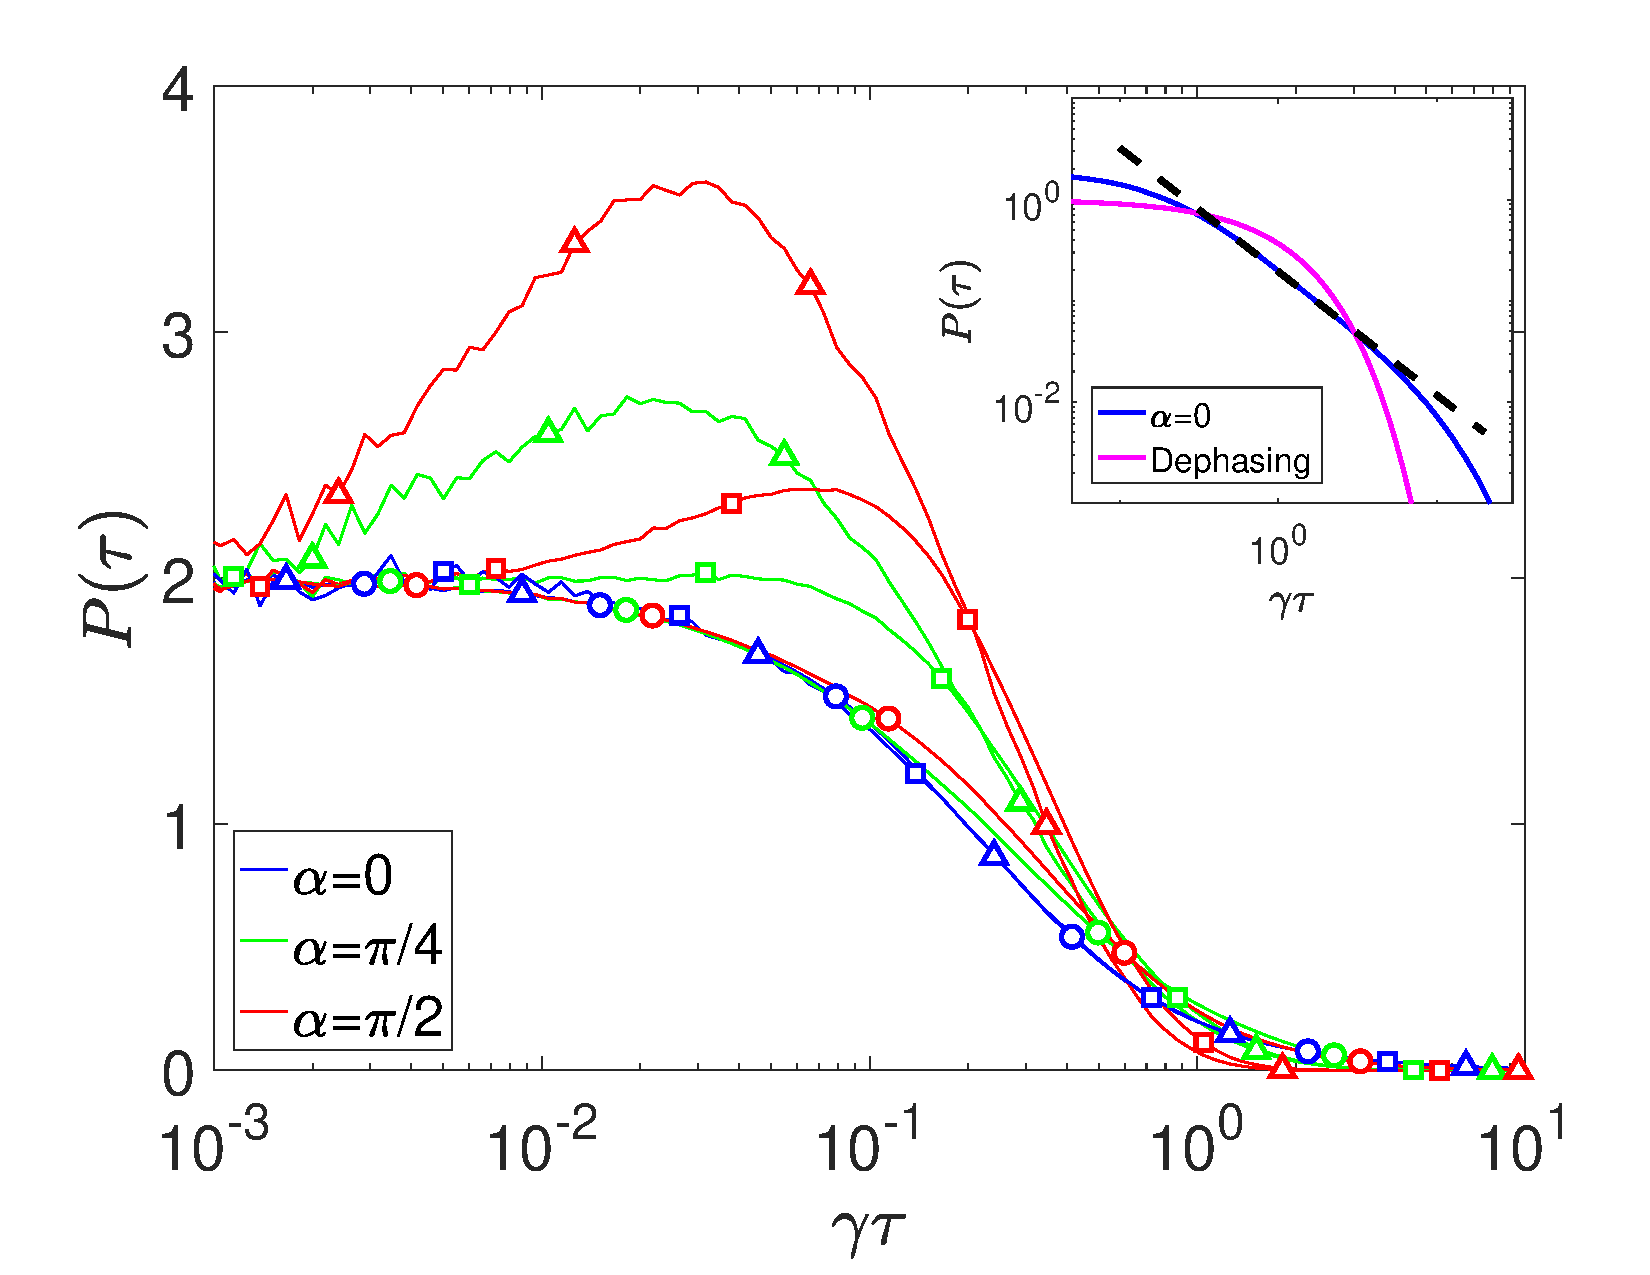
\includegraphics[scale=0.55]{anderson_prb_5}
	}
	\caption[Статистика распределения временных интервалов между последовательными во времени квантовыми скачками для разных режимов распространения волновых пакетов]{
		Статистика распределения временных интервалов между последовательными во времени квантовыми скачками. Синие кривые соответствуют случаю \(\alpha=0\), зелёные "--- \(\alpha = \frac{\pi}{4}\), красные "--- \(\alpha = \frac{\pi}{2}\). Разными символами показаны разные скорости диссипации \(\gamma\):  круги для \(\gamma=0.1\), квадраты для \(\gamma=0.01\), треугольники для \(\gamma=0.001\). Во вставке графика изображены распределения для неэрмитовых диссипаторов \cref{eq:anderson_diss_local} с \(\alpha=0\) (синяя кривая) и дефазирующей диссипации \cref{eq:anderson_diss_dephase} (в обоих случаях \(\gamma=0.1\)). Чёрная пунктирная линия "--- аппроксимация \(P(\tau) \sim \tau^{-1}\).
	}
	\label{fig:anderson_prb_5}
\end{figure}

Чтобы получить более полное представление о микроскопической динамике квантовых траекторий проанализируем статистику распределения временных интервалов между последовательными во времени квантовыми скачками (алгоритм \ref{alg:qt_jump}), обозначаемую \(P(\tau)\), где \(\tau\) "--- временной интервал между скачками.

Рассмотрим сначала случай неэрмитовых диссипаторов \cref{eq:anderson_diss_local} c \(\alpha=0\), когда локализация наиболее выражена, и наблюдается длительная циркуляция квантовых  траекторий на доминирующих Андерсоновских модах (рисунок \cref{fig:anderson_prb_2_1, fig:anderson_prb_2_2}). 
Для данного типа динамики в распределении времён между квантовыми скачками  характерно наличие сегмента, который можно приблизить степенным законом \(P(\tau) \sim \tau^{-1}\), что очень сильно отличается от классического распределения Пуассона, характерного для дефазирующей диссипации \cref{eq:anderson_diss_dephase} (рисунок \cref{fig:anderson_prb_5}, вставка).

Дополнительные особенности проявляются при варьировании фазы диссипатора \(\alpha\) (рисунок \cref{fig:anderson_prb_5}, основная часть).
При \(\alpha=0\), когда распространение волновых пакетов является диффузионным, распределение времён между скачками хорошо масштабируется со скоростью диссипации \(\gamma\) "--- все синие кривые с разным значением \(\gamma\) (разными символами) совпали на рисунке.
Данный результат объясняется тем, что единственный временной масштаб задаётся зависимыми от \(\gamma\) квантовыми скачками между разными Андерсоновскими модами.
При ненулевом значении фазы \(\alpha\) наблюдается совершенно другое распределение \(P(\tau)\). 
В то время как для умеренной скорости диссипации (\(\gamma = 0.1\)) распределения для \(\alpha = \frac{\pi}{4}\) и \(\alpha = \frac{\pi}{2}\) не сильно отличаются от кривых для \(\alpha=0\), при слабой диссипация (\(\gamma = 0.01, 0.001\)) наблюдается ярковыраженный максимум в распределении \(P(\tau)\).

Таким образом, в открытой квантовой системе Андерсона существуют нетривиальные режимы распространения волновых пакетов за счёт взаимодействия беспорядка и диссипации. Квантовые траектории демонстрируют диффузионные (при которых циркуляция в Андерсоновских модах прерывается квантовыми скачками) и баллистические режимы. Управляя фазой неэрмитовых диссипаторов, можно переключать данные режимы. В диффузионном режиме статистика времён между квантовыми скачками не является пуассоновской и имеет степенной интервал, что является следствием периодической синхронизации в модах Андерсона. Баллистическое распространение вводит вторую шкалу времени для скачков и ограничивает время циркуляции в модах Андерсона, что приводит к немонотонному распределению времён между скачками \cite{Yusipov2018}.

\section{Многочастичная локализация в открытых квантовых системах}\label{sec:ch2/prb_mbl}
Явление многочастичной локализации (MBL) основано на балансе между локализацией Андерсона, вызванной интерференцией волн, и взаимодействием между квантовыми частицами. Ожидается, что диссипация размывает интерференцию и разрушает этот баланс, в результате чего асимптотическое состояние уже открытой квантовой системы с гамильтонианом MBL не несёт признаков локализации. Для случая эрмитовой дефазирующей диссипации это действительно так: асимптотическое состояние такой системы является тривиальным и имеет максимально возможную энтропию в системе \cite{Levi2016, Fischer2016, Medvedyeva2016}. В данном разделе будет продемонстрировано, что система MBL может быть переведена в специфическое асимптотическое состояние, с признаками локализации, используя физически реализуемые неэрмитовые диссипативные операторы \cite{Diehl2008}, каждый из которых нетривиально действует на пару соседних сайтов решётки.

Гамильтониан системы с многочастичной локализацией описывает динамику \(\frac{N}{2}\) бесспиновых фермионов на решётке размером \(N\) (\(N\) предполагается всегда чётным).  Гамильтониан системы имеет вид \cite{Levi2016, Fischer2016, Medvedyeva2016}:
\begin{equation}
	\label{eq:mbl_H}
	\begin{gathered}
		H = \sum_{n=1}^{N} h_n b^{\dagger}_n b_n + \sum_{n=1}^{N-1} b^{\dagger}_n b_n b^{\dagger}_{n+1} b_{n+1} - \sum_{n=1}^{N-1} \left( b^{\dagger}_n b_{n+1} + b^{\dagger}_{n+1} b_n \right) ,
	\end{gathered}
\end{equation}
где \(b_n\) и \(b^{\dagger}_n\) "--- операторы уничтожения и создания фермиона на \(n\)-ом сайте решётки соответственно, \(b^{\dagger}_n b_n\) "--- оператор числа частиц на сайте \(n\).
В каждом узле решётки на фермионы действуют случайные потенциалы \(h_n\) (первое слагаемое в правой части). Фермионы, которые находятся в соседних сайтах решётки, взаимодействуют между собой (второе слагаемое в правой части). Третье слагаемое в правой части отвечает за перемещение фермионов между сайтами решётки. Значения случайных потенциалов \(h_n\) равномерно распределены в интервале \(\left[-h, h \right]\). Для данной системы известно \cite{Pal2010}, что переход к многочастичной локализации осуществляется при \(h > h_{MBL} \approx 3.6\). Число состояний в системе определяется числом сочетаний \(\frac{N}{2}\) из \(N\):
\begin{equation}
	\label{eq:mbl_num_states}
	\begin{gathered}
		S = \frac{N!}{ (\frac{N}{2})! (\frac{N}{2})!}.
	\end{gathered}
\end{equation}
Открытая квантовая система описывается уравнением Линдблада \cref{eq:GKSL_base, eq:GKSL_lindbladian}. Унитарная эволюция осуществляется под воздействием гамильтониана \cref{eq:mbl_H}.
Если для описания взаимодействия с окружающей средой взять диссипативные операторы следующего вида \cite{Levi2016, Fischer2016, Medvedyeva2016}:
\begin{equation}
	\label{eq:mbl_diss_dephase}
	\begin{gathered}
		V_k = b^{\dagger}_k b_k,
	\end{gathered}
\end{equation}
то это приведёт систему в тривиальное асимптотическое состояние с максимальной энтропией: \(\rho^A = \frac{\idmtx}{S}\) (как и любые другие эрмитовые диссипаторы). 

C другой стороны, чтобы привести систему в состояние, отличное от тривиального, можно использовать такие неэрмитовые диссипативные операторы \(V_i\), которые гарантируют выполнения условия \(V_i \left| \phi_i \right\rangle = 0\), где \(\left| \phi_i \right\rangle\) "--- собственный вектор гамильтониана \cref{eq:mbl_H}. В этом случае асимптотическое состояние равновесие будет нетривиальным: \(\rho^A = \left| \phi_i \right\rangle \left\langle \phi_i \right| \). Однако такие диссипаторы не являются физически реализуемыми. В качестве альтернативы будут рассматриваться экспериментально релевантные неэрмитовые диссипаторы \cite{Diehl2008}:
\begin{equation}
	\label{eq:mbl_diss_diehl}
	\begin{gathered}
		V_k = ( b^\dagger_k + b^\dagger_{k+1}) \left( b_k - b_{k+1} \right),
	\end{gathered}
\end{equation}
аналогичные неэрмитовым диссипаторам, рассмотренным в моделе Андерсона. 
Данный тип диссипаторов синхронизирует динамику на соседних сайтах, за счёт рециркуляции антисимметричных противофазных состояний в симметричные и синфазные.
Их физическая реализация предложена в работе \cite{Marcos2012}.

В общем случае будет рассмотрена ситуация, когда в системе одновременно есть оба типа диссипации "--- \cref{eq:mbl_diss_dephase} и \cref{eq:mbl_diss_diehl} cо скоростями \(\gamma^d\) и \(\gamma^l\) соответственно. В этом случае общее количество диссипаторов будет \(K = 2 N - 1\) (\(N\) дефазирующих и \(N-1\) неэрмитовых). 

Для наблюдения за сходимостью матрицы плотности к асимптотическому состоянию использовалось численное интегрирование уравнения \cref{eq:GKSL_lindbladian}.
В качестве начального условия рассматривается состояние \(\rho(t_0) =\left| \phi(t_0) \right\rangle \left\langle \phi(t_0) \right| \), где \(\left| \phi(t_0) \right\rangle = \left| 1010\ldots10 \right\rangle\) "--- состояние, при котором все фермионы находятся в нечётных сайтах решётки.
Для отыскания асимптотического состояния равновесия \(\rho^A\) использовались спектральные методы для отыскания собственного вектора, который соответствует нулевому собственному числу Линдбладиана \(L\) в уравнении \cref{eq:GKSL_lindbladian} \cite{Nation2015, eigenweb, Hernandez2005}. 
Используя данный метод были получены результаты для \(N=8\) и \(10\) (число состояний системы \(S=70\) и  \(252\) соответственно \cref{eq:mbl_num_states}).
Анализ систем с \(N>10\) были выполнен соавторами основополагающей работы \cite{Vakulchyk2018} и также будет представлен в данном разделе для полноты приводимых результатов по многочастичной локализации в открытых квантовых системах.
Количество случайных реализаций беспорядка: \(N_r=10^4\) для \(N=8\), \(N_r=4 \cdot 10^3 \) для \(N=10, 16\).

Одной из характеристик, позволяющим численно оценивать многочастичную локализацию является дисбаланс (imbalance), который вычисляется следующим образом:
\begin{equation}
	\label{eq:mbl_imbalance}
	\begin{gathered}
		\mathcal{I}(t) = \frac{\mathcal{N}_o(t) - \mathcal{N}_e(t)}{N/2},
	\end{gathered}
\end{equation}
где \(\mathcal{N}_o(t)\) и \(\mathcal{N}_e(t)\) "--- количество фермионов на нечётных и чётных сайтах решётки в момент времени \(t\) соответственно. Данная характеристика измеряется в реальных экспериментах \cite{Schreiber2015, Choi2016, Bordia2017, Lschen2017}.
\begin{figure}[h]
	\centerfloat{
		\hfill
		\subcaptionbox[List-of-Figures entry]{\label{fig:mbl_imbalance_1_1}}{%
			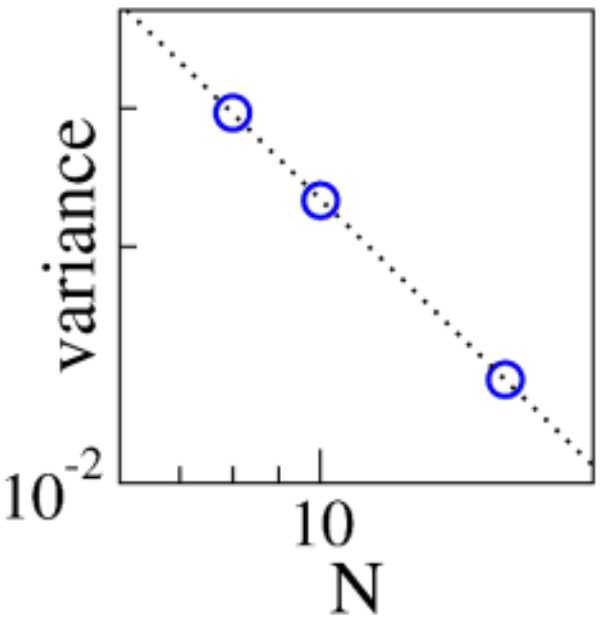
\includegraphics[width=0.35\linewidth]{mbl_imbalance_1_1}}
		\hfill
		\subcaptionbox{\label{fig:mbl_imbalance_1_2}}{%
			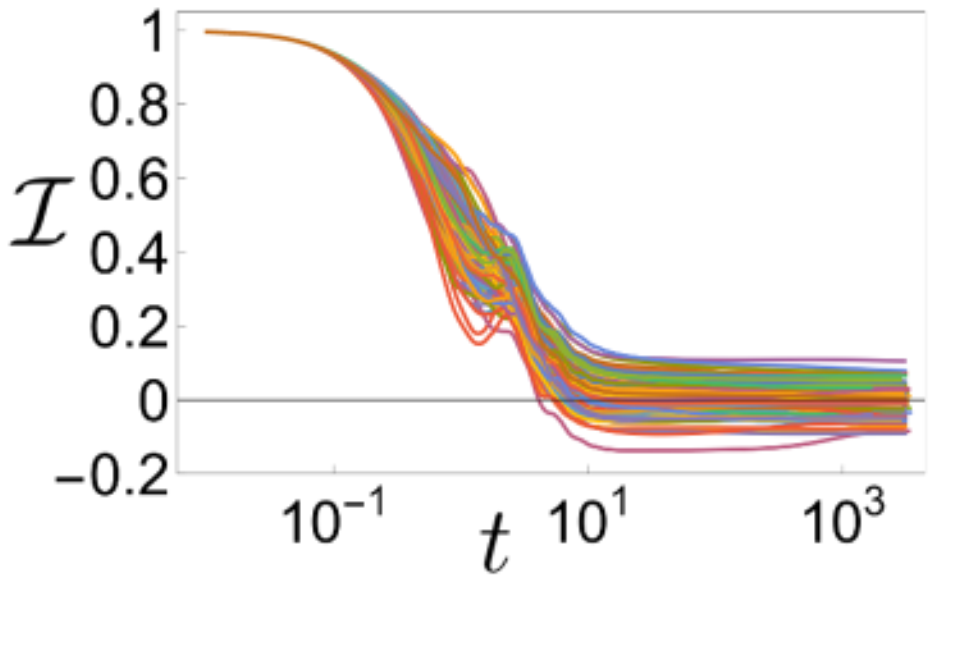
\includegraphics[width=0.53\linewidth]{mbl_imbalance_1_2}}
	}
	\legend{}
	\caption[Масштабирование дисперсии распределения дисбаланса и его эволюция во времени в модели MBL]
	{
		(a): Масштабирование дисперсии распределения \( P(\mathcal{I}) \) для силы беспорядка \(h=3\), чёрная пунктирная линия "--- степенной закон \(N^{2 \beta_h}\); (б): Эволюция имбаланса для 100 реализаций беспорядка с \(h=20\) и \(N=32\).
	}
	\label{fig:mbl_imbalance_1}
\end{figure}
\begin{figure}[h]
	\centerfloat{
		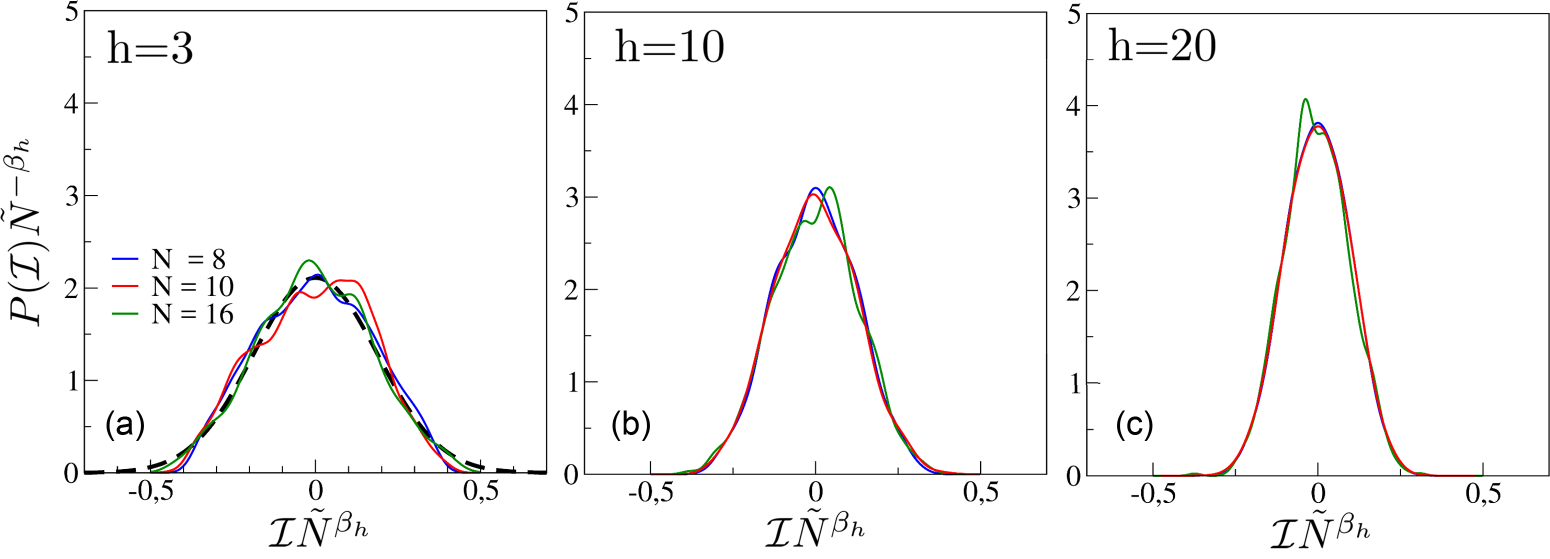
\includegraphics[scale=0.4]{mbl_imbalance_2}
	}
	\caption[Плотность распределения дисбаланса для разных значений беспорядка и разного количества частиц]{
		Функция распределение вероятностей дисбаланса \(\mathcal{I}\) для различных значений силы беспорядка \(h\) и количества фермионов в системе c учётом шкалирования \cref{eq:mbl_imbalance_scale} относительно значения \(\tilde{N} = \frac{N}{8}\). Значения степени шкалирования \(\beta_h = 0.55\) для \(h=3\) и \(\beta_h = 0.8\) для \(h=10, 20\).
	}
	\label{fig:mbl_imbalance_2}
\end{figure}

В случае, когда в системе есть только дефазирующая диссипация (\(\gamma^d \ne 0\), \(\gamma^l = 0\)), асимптотическое значение дисбаланса равно нулю, что следует из вида асимптотической матрицы плотности \(\rho^A = \frac{\idmtx}{S}\), диагональные элементы которой соответствуют вероятности нахождения системы в заданном состоянии.
Когда диссипация неэрмитова (\(\gamma^d = 0\), \(\gamma^l \ne 0\)), асимптотическое состояние зависит от текущей реализации беспорядка в системе, а асимптотический дисбаланс является случайной величиной. 
Дисбаланс можно рассматривать как сумму, состоящую из \(\frac{N}{2}\) случайных величин \(\xi_n = o_{2n - 1} -  o_{2n}\) (\(n=1,\cdots,\frac{N}{2}\)), где \(o_n\) "--- заселённость \(n\)-го узла. Поскольку данные случайные величины являются коррелированными, их суммы не подчиняются центральной предельной теореме \cite{billingsley2012}. Исследуем теперь функцию плотности распределения вероятности дисбаланса \( P(\mathcal{I}) \) в зависимости от параметра беспорядка \(h\). Для разных размеров систему введём следующую систему шкалирования:
\begin{equation}
	\label{eq:mbl_imbalance_scale}
	\begin{gathered}
		\mathcal{I} \to N^{\beta_h} \mathcal{I},\\
		P(\mathcal{I}) \to \frac{P(N^{\beta_h} \mathcal{I})}{N^{\beta_h}},
	\end{gathered}
\end{equation}
где \(\beta_h\) является функцией от беспорядка \(h\) (\(\beta_h = \frac{1}{2}\) соответствует случаю, когда выполняется центральная предельная теорема).
Значения экспоненты могут быть оценены путём вычисления дисперсии \(P(\mathcal{I})\) для различных \(N\) и затем аппроксимации полученной зависимости степенным законом \(N^{2 \beta_h}\) (рисунок \cref{fig:mbl_imbalance_1_1}). Было обнаружено, что для эргодического режима (\(h=3\)) значение \(\beta_h = 0.55\), для режима многочастичной локализации (\(h=10, 20\)) значение \(\beta_h = 0.8\).
На рисунке \cref{fig:mbl_imbalance_2} изображено шкалирование \cref{eq:mbl_imbalance_scale} для разных значений беспорядка \(h\) и разного количества фермионов в системе. Шкалирование выполнялось относительно значения \(\tilde{N} = \frac{N}{8}\).
Для дополнительного исследования рассмотрим некоторое множество случайных независимых наблюдаемых \(\{x_1, x_2, \cdots, x_N\}\), с равномерным распределением, нормировкой на сумму выбранных случайных значений: \(\sum_{n=1}^{N}x_n = \frac{N}{2}\) и ограничением: \(\forall x_n < 1\) (не более одной частицы на одном сайте решётки). Результат выборки для такого распределения для \(N=16\) представлен на рисунке \cref{fig:mbl_imbalance_2} для случая \(h=3\) (пунктирная линия) и хорошо согласуется с кривой для плотности вероятности дисбаланса. 

Второй характеристикой, которая будет использоваться для изучения явления многочастичной локализации в открытых квантовых системах, является энтропия запутанности операторного пространства (OSEE "--- operator"--~space entanglement entropy). Обозначается как \(S^{\natural}\). 
Эта характеристика впервые была введена в работе \cite{Prosen2007} как операторное обобщение энтропии пространственной запутанности (определённой для чистых состояний).
Для вычисления OSEE необходимо разбить цепочку на две (в случае рассматриваемой MBL системы "--- равные) части и вычислить разложение Шмидта матрицы плотности:
\begin{equation}
	\label{eq:mbl_osee_shcmidt}
	\begin{gathered}
		\rho = \sum_{k} \sqrt{\mu_k} C_k \otimes D_k, 
	\end{gathered}
\end{equation}
где операторы \(C_k\) и \(D_k\) нетривиально действуют на левую и правую подсистемы и образуют полный базис Гильберта"--~Шмидта в соответствующем подпространстве.
Нормированные коэффициенты \(\bar{\mu}_k\) определяют значение OSEE:
\begin{equation}
	\label{eq:mbl_osee}
	\begin{gathered}
		S^{\natural} = - \sum_{k} \bar{\mu}_k \log_2{\bar{\mu}_k}. 
	\end{gathered}
\end{equation}
Если квантовая система находится в чистом состоянии, то значение OSEE вдвое превышает значение стандартной энтропии запутанности \cite{Znidaric2008_entropy}.

\begin{figure}[h]
	\centerfloat{
		\hfill
		\subcaptionbox[List-of-Figures entry]{\label{fig:mbl_osee_1_1}}{%
			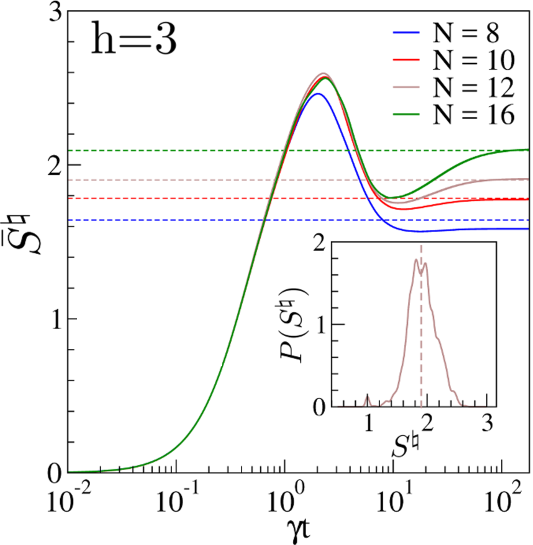
\includegraphics[width=0.3\linewidth]{mbl_osee_1_1}}
		\hfill
		\subcaptionbox{\label{fig:mbl_osee_1_2}}{%
			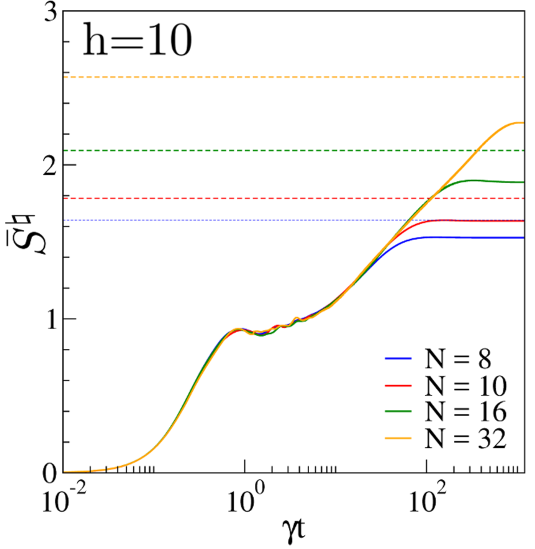
\includegraphics[width=0.3\linewidth]{mbl_osee_1_2}}
		\hfill
		\subcaptionbox{\label{fig:mbl_osee_1_3}}{%
			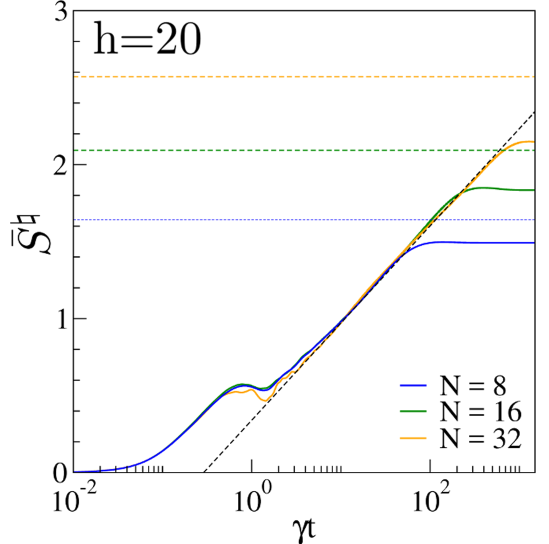
\includegraphics[width=0.31\linewidth]{mbl_osee_1_3}}
	}
	\legend{}
	\caption[Энтропия запутанности операторного пространства (OSEE)]
	{
		Усредненное значение энтропии запутанности операторного пространства (OSEE) \(S^{\natural}(t)\) как функции времени для \(h=3\) (а), \(h=10\) (б), \(h=20\) (в). Цветные пунктирные линии соответствуют значениям OSEE для термализованной системы. Вставка для случая \(h=3\) "--- функция плотности вероятности распределения OSEE для \(N=12\). Чёрная пунктирная линия на рисунке для \(h=20\) соответствует закону \(\frac{1}{2}\log_2(t) + const\).
	}
	\label{fig:mbl_osee_1}
\end{figure}

Было обнаружено, что в эргодической фазе (когда \(h=3\)) усреднённое по беспорядку значение OSEE \(\bar{S}^{\natural}\) со временем насыщается до значения \(S^{\natural}(\idmtx)\), когда все состояния системы равновероятны (рисунок \cref{fig:mbl_osee_1_1}).
То есть наступает эффективная термализация системы, при отсутствии дефазирующей диссипации.
Энтропия запутанности операторного пространства зависит от текущей реализации беспорядка в системе и от реализации к реализации группируется возле определённого, не максимального значения (рисунок \cref{fig:mbl_osee_1_1}, вставка).
Эволюция во времени OSEE начинается с роста, который, при отсутствии диссипации в системе, достиг бы предельного значения \(S^\natural_{\lim} = N - 1\) \cite{Page1993}.
Однако,  после момента времени \(t=\gamma^{-1}\) вклад диссипативной части линдбладиана \cref{eq:GKSL_base} становится значительным и в конечном итоге приводит OSEE к асимптотическому значению \(S^\natural(\rho^A) \ll S^\natural_{\lim}\).

В случае, когда в системе наблюдается многочастичная локализация (\(h=10, 20\)), усреднённое значение OSEE со временем сходится к значению, меньшему чем \(S^{\natural}(\idmtx)\) (рисунок \cref{fig:mbl_osee_1_2, fig:mbl_osee_1_3}).
Это объясняется тем,  в эргодической фазе все (даже удалённые) узлы «связаны» сохранением полного числа частиц (полного спина), в фазе MBL корреляции являются короткодействующими и ограничиваются длиной локализации \cite{Pal2010}. 
Следовательно, квантовая запутанность является короткодействующей в случае многочастичной локализации.
Примечательно, что, как и в случае энтропии запутанности в гамильтоновом случае \cite{Chiara2006, Znidaric2008, Bardarson2012, Serbyn2016}, релаксация OSSE до асимптотического значения сопровождается логарифмическим ростом \(S^{\natural} \sim \log(t)\) (чёрная пунктирная линия на рисунке \cref{fig:mbl_osee_1_3}) "--- свойством, обнаруженным ранее в работе \cite{Medvedyeva2016}, где рассматривалась открытая модель MBL c дефазирующей диссипацией.

Третьей характеристикой для изучения многочастичной локализации является соотношение последовательных уровней \(r\) (RCLS "--- ratio of consecutive level spacing) для асимптотической матрицы плотности.
Согласно теории квантового хаоса \cite{Haake2018}, одной из общепризнанных характеристик квантового хаоса является статистика уровней собственных энергий:
\begin{equation}
	\label{eq:mbl_energy_levels}
	\begin{gathered}
		\delta_j = \lambda_{j+1} - \lambda_{j}, 
	\end{gathered}
\end{equation}
где множество \(\{\lambda_j\}\) "--- отсортированные по возрастанию собственные числа гамильтониана системы.
Если статистика уровней собственных энергий совпадает с распределением Пуассона, то динамика в системе является регулярной.
Если же распределение собственных энергий совпадает с распределением Вигнера"--~Дайсона, то в системе есть квантовый хаос.
Следуя этому, можно ожидать, что в эргодической фазе будет иметь место распределение Вигнера"--~Дайсона и в случае многочастичной локализации будет распределение Пуассона \cite{Oganesyan2007, Serbyn2016}.
Однако, данные критерии предполагают однородную плотность уровней собственных энергий, что не выполняется для рассматриваемой модели \cref{eq:mbl_H}.
Чтобы обойти данное ограничение, рассматривается распределение соотношений \(r_j\), которые определяются следующим образом:
\begin{equation}
	\label{eq:mbl_ratio}
	\begin{gathered}
		\delta_j = \lambda_{j+1} - \lambda_{j}, \\
		z_j = \frac{\delta_{j+1}}{\delta_{j}}, \\
		r_j = \min\left(z_j, \frac{1}{z_j} \right),
	\end{gathered}
\end{equation}
где \(\lambda_{j}\) - собственные числа рассматриваемой матрицы. 
Распределения \(r_j\) не зависят от локальной плотности уровней \cite{Oganesyan2007}.
Из литературы \cite{Atas2013} известны значения RCLS \cref{eq:mbl_ratio} для случайных величин с распределением Пуассона, для случайных матриц \cite{mehta2004random} из гауссова ортогонального ансамбля (GOE "--- Gaussian orthogonal ensembles) и случайных матриц из гауссова унитарного ансамбля (GUE "--- Gaussian unitary ensembles):

\begin{table} [htbp]
	\centering
	\begin{threeparttable}% выравнивание подписи по границам таблицы
		\caption{Значения среднего соотношения последовательных уровней для случайных матриц}\label{tab:mbl_ratio_constants}%
		\begin{tabular}{| p{7cm} || p{6cm}l |}
			\hline
			\hline
			Тип распределения   & \centering  \(r\) & \\
			\hline
			Poisson &\centering      0.386 	 &   \\
			GOE  	&\centering      0.536   &   \\
			GUE 	&\centering    	 0.603 	 &   \\
			\hline
			\hline
		\end{tabular}
	\end{threeparttable}
\end{table}

\begin{figure}[h]
	\centerfloat{
		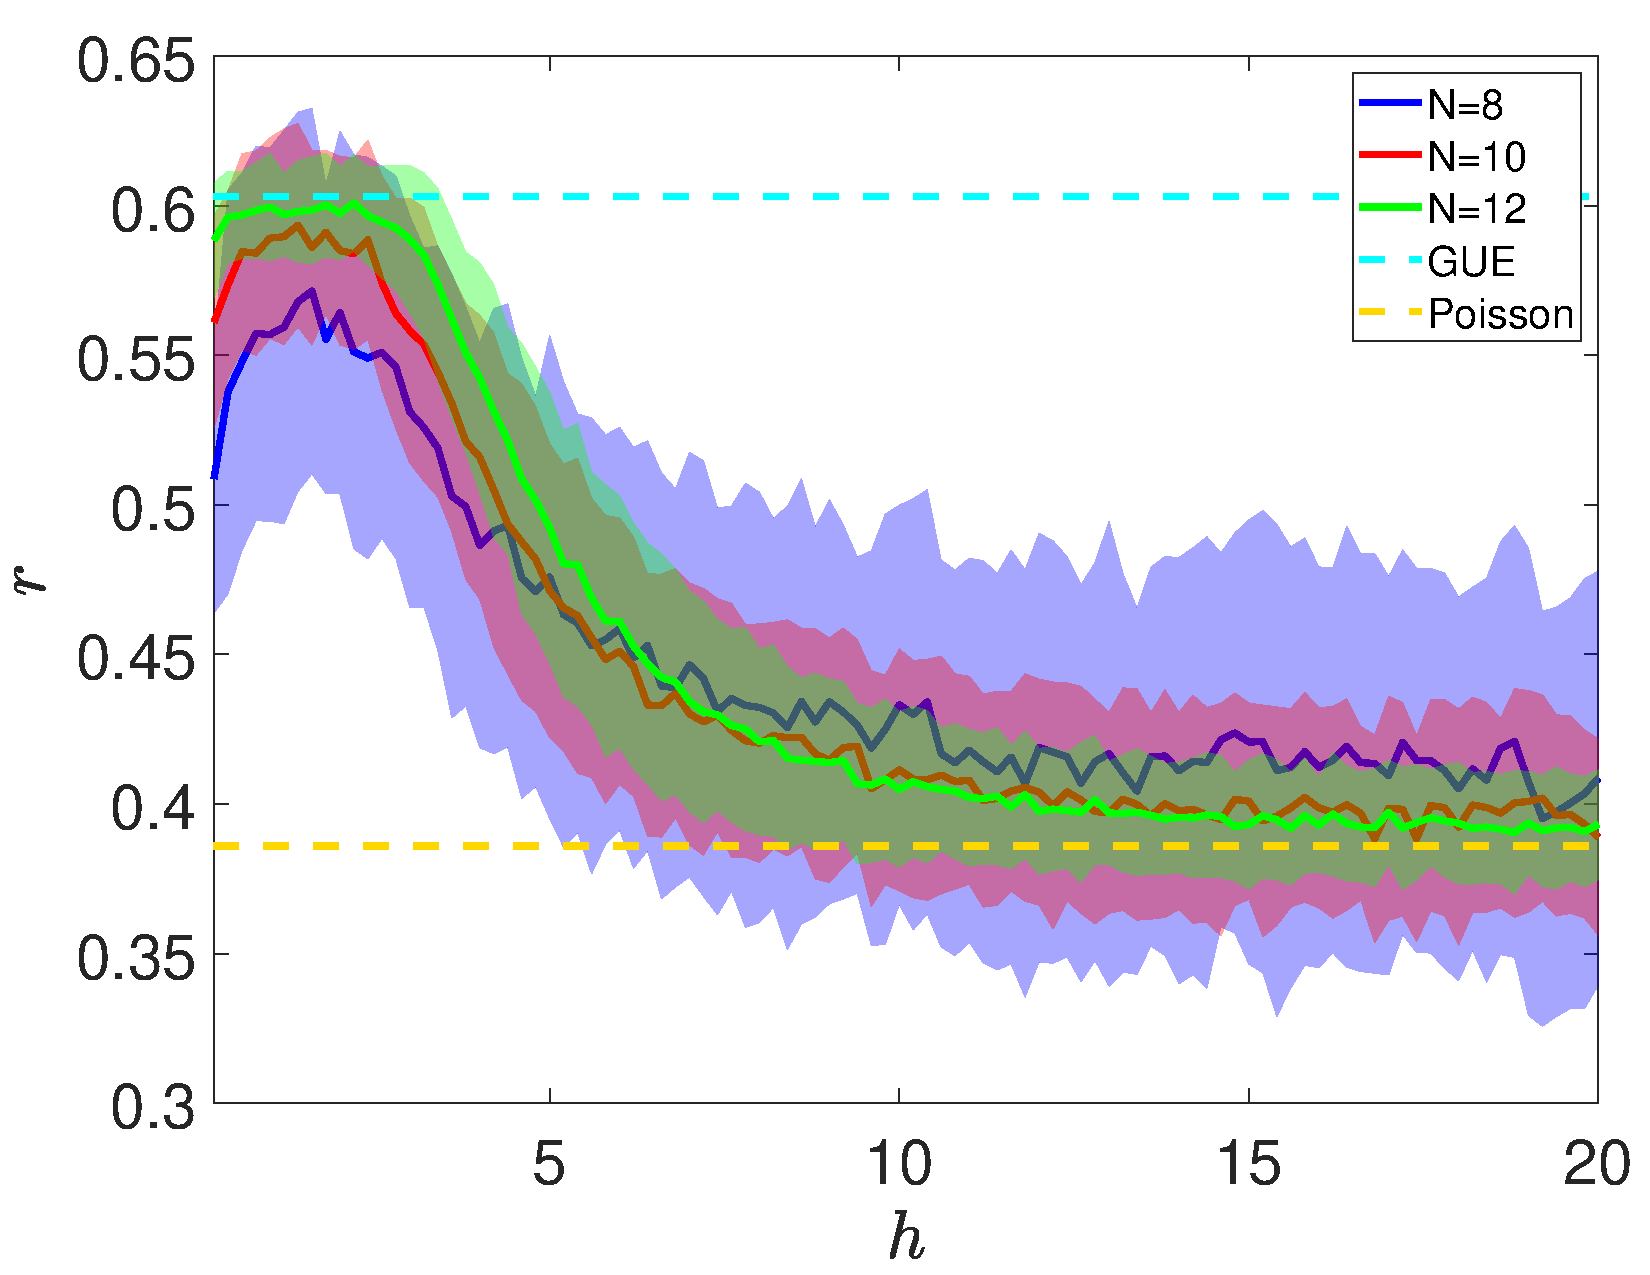
\includegraphics[scale=0.55]{mbl_ratio}
	}
	\caption[Соотношение последовательных уровней для асимптотической матрицы плотности в зависимости от силы беспорядка в системе]{
		Соотношение последовательных уровней \cref{eq:mbl_ratio} для асимптотической матрицы плотности \(\rho^A\) в зависимости от силы беспорядка \(h\). Сплошными линиями обозначено усреднённое значение \(r\) по \(N_r=100\) реализациям беспорядка для каждого значения \(h\). Области соответствующего цвета обозначают стандартное отклонение распределения \(r\). Пунктирные линии соответствуют значениям \(r_{Poisson}\) и \(r_{GUE}\) (таблица \cref{tab:mbl_ratio_constants}).
	}
	\label{fig:mbl_ratio}
\end{figure}

В работе \cite{Prosen2013} было обнаружено, что переход от регулярной динамики к хаотической соответствует переходу от распределения Пуассона к GUE.
Для данной системы было обнаружено, что в эргодической фазе (\(h=3\)) значения RCLS \cref{eq:mbl_ratio} для асимптотической матрицы плотности \(\rho^A\) группируется возле \(r_{GUE}\), а в случае сильной многочастичной локализации (\(h=20\)) значения \(r\) приближаются к \(r_{Poisson}\) (рисунок \cref{fig:mbl_ratio}). Это соответствие улучшается с увеличением \(N\).

\begin{figure}[h]
	\centerfloat{
		\hfill
		\subcaptionbox[List-of-Figures entry]{\label{fig:mbl_rho_1}}{%
			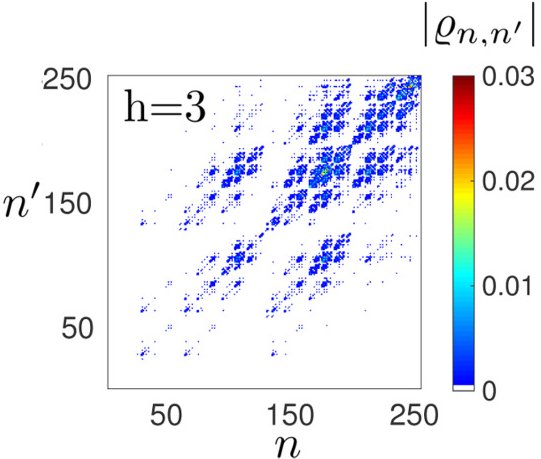
\includegraphics[width=0.5\linewidth]{mbl_rho_1}}
		\hfill
		\subcaptionbox{\label{fig:mbl_rho_2}}{%
			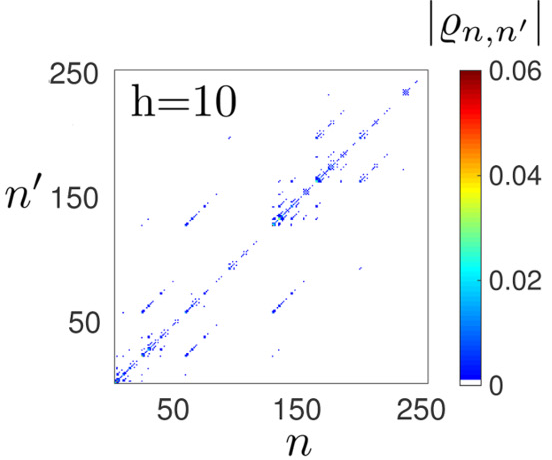
\includegraphics[width=0.5\linewidth]{mbl_rho_2}}
	}
	\legend{}
	\caption[Структура асимптотической матрицы плотности для эргодической фазы и случая многочастичной локализации]
	{
		Абсолютные значения асимптотической матрицы плотности \(\rho^A\) для отдельно взятой реализации беспорядка и силы беспорядка \(h=3\) (a) и \(h=10\) (б). На рисунках отмечены только элементы, большие \(10^{-5}\).
	}
	\label{fig:mbl_rho}
\end{figure}

Так же была рассмотрена структура асимптотических матриц плотности.
В эргодической фазе \(h=3\) наблюдается хорошо развитая недиагональная структура (рисунок \cref{fig:mbl_rho_1}), а в случае многочастичной локализации "--- имеет место почти диагональная структура (рисунок \cref{fig:mbl_rho_2}) похожая на ту, которая была обнаружена в разделе \cref{sec:ch2/prl} и соответствующей работе \cite{Yusipov2017}.

\begin{figure}[h]
	\centerfloat{
		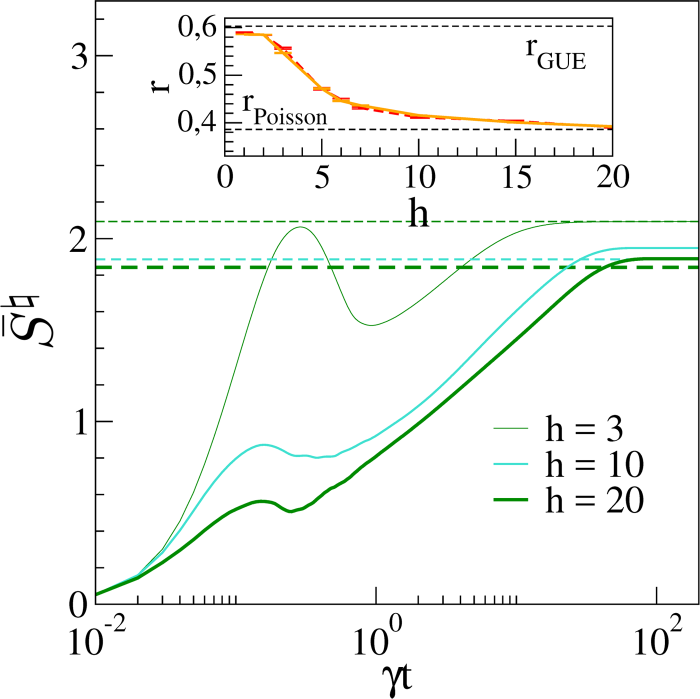
\includegraphics[scale=0.6]{mbl_both_diss}
	}
	\caption[Эволюция во времени энтропии запутанности операторного пространства и зависимость соотношения последовательных уровней асимптотической матрицы плотности от силы беспорядка для смешанной диссипации (дефазирующая и неэрмитовая)]{
		Эволюция во времени энтропии запутанности операторного пространства для смешанной диссипации (дефазирующая и неэрмитовая) "--- сплошные линии, пунктирные линии "--- значения \(S^\natural\) для термализованной системы, в которой есть только неэрмитовая диссипация. Размер системы \(N=16\). Вставка "--- 
		соотношение последовательных уровней \cref{eq:mbl_ratio} для асимптотической матрицы плотности \(\rho^A\) в зависимости от силы беспорядка \(h\) для смешанной диссипации (оранжевая сплошная линия) и неэрмитовой диссипации (красная пунктирная линия).
	}
	\label{fig:mbl_both_diss}
\end{figure}

Рассмотрим теперь ситуацию, когда в системе есть оба типа диссипации: дефазирующая \cref{eq:mbl_diss_dephase} с \(\gamma^d = 0.1\) и неэрмитова диссипация c \(\gamma^l = 0.1\). 
На рисунке \cref{fig:mbl_both_diss} изображена эволюция во времени энтропии запутанности операторного пространства для данного случая (сплошные линии). Пунктирные линии соответствуют значениям \(S^\natural\) для термализованной системы, в которой есть только неэрмитовая диссипация (рисунок \cref{fig:mbl_osee_1}). 
Из графика видно, что OSEE асимптотической матрицы плотности \(\rho^A\) немного изменяется в фазе многочастичной локализации \(h=10, 20\) и остаётся постоянной в эргодической фазе \(h=3\) при наличии в системе дефазирующей диссипации. 
Также на вставке рисунка \cref{fig:mbl_both_diss} для случая со смешанной диссипацией оранжевой сплошной линией изображена эволюция соотношения последовательных уровней \cref{eq:mbl_ratio} для асимптотической матрицы плотности \(\rho^A\) в зависимости от силы беспорядка \(h\). 
Данная зависимость практически идентична случаю с отсутствием дефазирующей диссипации (рисунок \cref{fig:mbl_ratio}) - красная пунктирная линия на вставке.
Таким образом, если ввести в систему с дефазировкой неэрмитовую диссипацию вида \cref{eq:mbl_diss_diehl} можно восстановить особенности локализации в открытых квантовых системах с MBL гамильтонианом.

В данном разделе были представлены три количественных идентификатора многочастичной локализации (MBL) в открытых квантовых системах.
Статистика дисбаланса может быть измерена в реальных физических экспериментах \cite{Schreiber2015, Choi2016, Bordia2017, Lschen2017}, но требует изучения систем разных размеров. 
Энтропия запутанности операторного пространства (OSEE) указывает на различия между эргодической фазой и многочастичной локализацией как в асимптотическом пределе, так и в процессе релаксации к нему.
Соотношение последовательных уровней (RCLS) для асимптотической матрицы плотности связывает многочастичную локализацию и теорию квантового хаоса \cite{Prosen2013, Haake2018}. 
Неэрмитовая диссипация, нетривиально действующая на соседних сайтах пытается построить классические и квантовые корреляции между далеко расположенными сайтами, и достаточно слабая дефазировка не может их разрушить. 
В то же время механизмы MBL, индуцированные гамильтонианом, пытаются ограничить корреляции длиной локализации. 
В результате баланса между этими факторами возникает асимптотическое состояние со следами локализации.

\section{Выводы по главе}\label{sec:ch2/results}
В данной главе исследовался феномен локализации в открытых квантовых системах.
\begin{itemize}[beginpenalty=10000] % https://tex.stackexchange.com/a/476052/104425
	\item Обнаружено явление Андерсоновской локализации в открытых квантовых системах. Диссипация может быть использована для создания нетривиальных устойчивых состояний, в которых доминируют несколько локализованных андерсоновских мод пространственно-неоднородного гамильтониана \cite{Yusipov2017}.
	\item В открытой квантовой системе с локализацией Андерсона существует механизм управления асимптотическим состоянием системы. Оно может быть локализовано в любом месте спектра гамильтониана, за счёт управляемой синтетической диссипации. Полученные таким образом состояния являются устойчивыми к дефазирующей диссипации \cite{Vershinina2017}.
	\item В открытой квантовой системе с локализацией Андерсона существуют различные типы распространения волновых пакетов. В частности, баллистический режим, вызванный суммарным взаимодействием беспорядка и диссипации \cite{Yusipov2018}. 
	\item При введении специальной физически релевантной диссипации в модель с многочастичной локализацией, система будет сходиться в новое нетривиальное асимптотическое состояние, которое может иметь следы многочастичной локализации (индуцированной свойствами многочастичного гамильтониана), даже в присутствии локальной декогеренции. Предложены новые численные критерии для детектирования многочастичной локализации "--- статистика дисбаланса, энтропия запутанности операторного пространства и соотношение последовательных уровней для асимптотической матрицы плотности \cite{Vakulchyk2018}.
\end{itemize}


%\section{Одиночное изображение}\label{sec:ch2/sec1}
%
%\begin{figure}[ht]
%  \centerfloat{
%    \includegraphics[scale=0.27]{latex}
%  }
%  \caption{TeX.}\label{fig:latex}
%\end{figure}
%
%Для выравнивания изображения по-центру используется команда \verb+\centerfloat+, которая является во
%многом улучшенной версией встроенной команды \verb+\centering+.
%
%\section{Длинное название параграфа, в котором мы узнаём как сделать две картинки с~общим номером и названием}\label{sec:ch2/sect2}
%
%А это две картинки под общим номером и названием:
%\begin{figure}[ht]
%  \begin{minipage}[b][][b]{0.49\linewidth}\centering
%    \includegraphics[width=0.5\linewidth]{knuth1} \\ а)
%  \end{minipage}
%  \hfill
%  \begin{minipage}[b][][b]{0.49\linewidth}\centering
%    \includegraphics[width=0.5\linewidth]{knuth2} \\ б)
%  \end{minipage}
%  \caption{Очень длинная подпись к изображению,
%      на котором представлены две фотографии Дональда Кнута}
%  \label{fig:knuth}
%\end{figure}
%
%Те~же~две картинки под~общим номером и~названием,
%но с автоматизированной нумерацией подрисунков:
%\begin{figure}[ht]
%    \centerfloat{
%        \hfill
%        \subcaptionbox[List-of-Figures entry]{Первый подрисунок\label{fig:knuth_2-1}}{%
%            \includegraphics[width=0.25\linewidth]{knuth1}}
%        \hfill
%        \subcaptionbox{\label{fig:knuth_2-2}}{%
%            \includegraphics[width=0.25\linewidth]{knuth2}}
%        \hfill
%        \subcaptionbox{Третий подрисунок, подпись к которому
%        не~помещается на~одной строке}{%
%            \includegraphics[width=0.3\linewidth]{example-image-c}}
%        \hfill
%    }
%    \legend{Подрисуночный текст, описывающий обозначения, например. Согласно
%    ГОСТ 2.105, пункт 4.3.1, располагается перед наименованием рисунка.}
%    \caption[Этот текст попадает в названия рисунков в списке рисунков]{Очень
%    длинная подпись к второму изображению, на~котором представлены две
%    фотографии Дональда Кнута}\label{fig:knuth_2}
%\end{figure}
%
%На рисунке~\cref{fig:knuth_2-1} показан Дональд Кнут без головного убора.
%На рисунке~\cref{fig:knuth_2}\subcaptionref*{fig:knuth_2-2}
%показан Дональд Кнут в головном уборе.
%
%Возможно вставлять векторные картинки, рассчитываемые \LaTeX\ <<на~лету>>
%с~их~предварительной компиляцией. Надписи в таких рисунках будут выполнены
%тем же~шрифтом, который указан для документа в целом.
%На~рисунке~\cref{fig:tikz_example} на~странице~\pageref{fig:tikz_example}
%представлен пример схемы, рассчитываемой пакетом \verb|tikz| <<на~лету>>.
%Для ускорения компиляции, подобные рисунки могут быть <<кешированы>>, что
%определяется настройками в~\verb|common/setup.tex|.
%Причём имя предкомпилированного
%файла и~папка расположения таких файлов могут быть отдельно заданы,
%что удобно, если не~для подготовки диссертации,
%то~для подготовки научных публикаций.
%\begin{figure}[ht]
%    \centerfloat{
%        \ifdefmacro{\tikzsetnextfilename}{\tikzsetnextfilename{tikz_example_compiled}}{}% присваиваемое предкомпилированному pdf имя файла (не обязательно)
%        \input{Dissertation/images/tikz_scheme.tikz}
%
%    }
%    \legend{}
%    \caption[Пример \texttt{tikz} схемы]{Пример рисунка, рассчитываемого
%        \texttt{tikz}, который может быть предкомпилирован}\label{fig:tikz_example}
%\end{figure}
%
%Множество программ имеют либо встроенную возможность экспортировать векторную
%графику кодом \verb|tikz|, либо соответствующий пакет расширения.
%Например, в GeoGebra есть встроенный экспорт,
%для Inkscape есть пакет svg2tikz,
%для Python есть пакет matplotlib2tikz,
%для R есть пакет tikzdevice.
%
%\section{Пример вёрстки списков}\label{sec:ch2/sec3}
%
%\noindent Нумерованный список:
%\begin{enumerate}
%  \item Первый пункт.
%  \item Второй пункт.
%  \item Третий пункт.
%\end{enumerate}
%
%\noindent Маркированный список:
%\begin{itemize}
%  \item Первый пункт.
%  \item Второй пункт.
%  \item Третий пункт.
%\end{itemize}
%
%\noindent Вложенные списки:
%\begin{itemize}
%  \item Имеется маркированный список.
%  \begin{enumerate}
%    \item В нём лежит нумерованный список,
%    \item в котором
%    \begin{itemize}
%      \item лежит ещё один маркированный список.
%    \end{itemize}
%  \end{enumerate}
%\end{itemize}
%
%\noindent Нумерованные вложенные списки:
%\begin{enumerate}
%  \item Первый пункт.
%  \item Второй пункт.
%  \item Вообще, по ГОСТ 2.105 первый уровень нумерации
%  (при необходимости ссылки в тексте документа на одно из перечислений)
%  идёт буквами русского или латинского алфавитов,
%  а второй "--- цифрами со~скобками.
%  Здесь отходим от ГОСТ.
%    \begin{enumerate}
%      \item в нём лежит нумерованный список,
%      \item в котором
%        \begin{enumerate}
%          \item ещё один нумерованный список,
%          \item третий уровень нумерации не нормирован ГОСТ 2.105;
%          \item обращаем внимание на строчность букв,
%          \item в этом списке
%          \begin{itemize}
%            \item лежит ещё один маркированный список.
%          \end{itemize}
%        \end{enumerate}
%
%    \end{enumerate}
%
%  \item Четвёртый пункт.
%\end{enumerate}
%
%\section{Традиции русского набора}
%
%Много полезных советов приведено в материале
%<<\href{https://kostyrka.ru/main/ru/typesetting-and-typography-crash-course-by-kostyrka/}{Краткий курс благородного набора}>>
%(автор А.\:В.~Костырка).
%Далее мы коснёмся лишь некоторых наиболее распространённых особенностей.
%
%\subsection{Пробелы}
%
%В~русском наборе принято:
%\begin{itemize}
%    \item единицы измерения, знак процента отделять пробелами от~числа:
%        10~кВт, 15~\% (согласно ГОСТ 8.417, раздел 8);
%    \item \(\tg 20\text{\textdegree}\), но: 20~{\textdegree}C
%        (согласно ГОСТ 8.417, раздел 8);
%    \item знак номера, параграфа отделять от~числа: №~5, \S~8;
%    \item стандартные сокращения: т.\:е., и~т.\:д., и~т.\:п.;
%    \item неразрывные пробелы в~предложениях.
%\end{itemize}
%
%\subsection{Математические знаки и символы}
%
%Русская традиция начертания греческих букв и некоторых математических
%функций отличается от~западной. Это исправляется серией
%\verb|\renewcommand|.
%\begin{itemize}
%%Все \original... команды заранее, ради этого примера, определены в Dissertation\userstyles.tex
%    \item[До:] \( \originalepsilon \originalge \originalphi\),
%    \(\originalphi \originalleq \originalepsilon\),
%    \(\originalkappa \in \originalemptyset\),
%    \(\originaltan\),
%    \(\originalcot\),
%    \(\originalcsc\).
%    \item[После:] \( \epsilon \ge \phi\),
%    \(\phi \leq \epsilon\),
%    \(\kappa \in \emptyset\),
%    \(\tan\),
%    \(\cot\),
%    \(\csc\).
%\end{itemize}
%
%Кроме того, принято набирать греческие буквы вертикальными, что
%решается подключением пакета \verb|upgreek| (см. закомментированный
%блок в~\verb|userpackages.tex|) и~аналогичным переопределением в
%преамбуле (см.~закомментированный блок в~\verb|userstyles.tex|). В
%этом шаблоне такие переопределения уже включены.
%
%Знаки математических операций принято переносить. Пример переноса
%в~формуле~\eqref{eq:equation3}.
%
%\subsection{Кавычки}
%В английском языке приняты одинарные и двойные кавычки в~виде ‘...’ и~“...”.
%В~России приняты французские («...») и~немецкие („...“) кавычки (они называются
%«ёлочки» и~«лапки», соответственно). ,,Лапки`` обычно используются внутри
%<<ёлочек>>, например, <<... наш гордый ,,Варяг``...>>.
%
%Французкие левые и правые кавычки набираются
%как лигатуры \verb|<<| и~\verb|>>|, а~немецкие левые
%и правые кавычки набираются как лигатуры \verb|,,| и~\verb|‘‘| (\verb|``|).
%
%Вместо лигатур или команд с~активным символом "\ можно использовать команды
%\verb|\glqq| и \verb|\grqq| для набора немецких кавычек и команды \verb|\flqq|
%и~\verb|\frqq| для набора французских кавычек. Они определены в пакете
%\verb|babel|.
%
%\subsection{Тире}
%%  babel+pdflatex по умолчанию, в polyglossia надо включать опцией (и перекомпилировать с удалением временных файлов)
%Команда \verb|"---| используется для печати тире в тексте. Оно несколько короче
%английского длинного тире. Кроме того, команда задаёт небольшую жёсткую отбивку
%от слова, стоящего перед тире. При этом, само тире не~отрывается от~слова.
%После тире следует такая же отбивка от текста, как и~перед тире. При наборе
%текста между словом и командой, за которым она следует, должен стоять пробел.
%
%В составных словах, таких, как <<Закон Менделеева"--~Клапейрона>>, для печати
%тире надо использовать команду \verb|"--~|. Она ставит более короткое,
%по~сравнению с~английским, тире и позволяет делать переносы во втором слове.
%При~наборе текста команда \verb|"--~| не отделяется пробелом от слова,
%за~которым она следует (\verb|Менделеева"--~|). Следующее за командой слово
%может быть  отделено от~неё пробелом или перенесено на другую строку.
%
%Если прямая речь начинается с~абзаца, то перед началом её печатается тире
%командой \verb|"--*|. Она печатает русское тире и жёсткую отбивку нужной
%величины перед текстом.
%
%\subsection{Дефисы и переносы слов}
%%  babel+pdflatex по умолчанию, в polyglossia надо включать опцией (и перекомпилировать с удалением временных файлов)
%Для печати дефиса в~составных словах введены две команды. Команда~\verb|"~|
%печатает дефис и~запрещает делать переносы в~самих словах, а~команда \verb|"=|
%печатает дефис, оставляя \TeX ’у право делать переносы в~самих словах.
%
%В отличие от команды \verb|\-|, команда \verb|"-| задаёт место в~слове, где
%можно делать перенос, не~запрещая переносы и~в~других местах слова.
%
%Команда \verb|""| задаёт место в~слове, где можно делать перенос, причём дефис
%при~переносе в~этом месте не~ставится.
%
%Команда \verb|",| вставляет небольшой пробел после инициалов с~правом переноса
%в~фамилии.
%
%\section{Текст из панграмм и формул}
%
%Любя, съешь щипцы, "--- вздохнёт мэр, "--- кайф жгуч. Шеф взъярён тчк щипцы
%с~эхом гудбай Жюль. Эй, жлоб! Где туз? Прячь юных съёмщиц в~шкаф. Экс-граф?
%Плюш изъят. Бьём чуждый цен хвощ! Эх, чужак! Общий съём цен шляп (юфть) "---
%вдрызг! Любя, съешь щипцы, "--- вздохнёт мэр, "--- кайф жгуч. Шеф взъярён тчк
%щипцы с~эхом гудбай Жюль. Эй, жлоб! Где туз? Прячь юных съёмщиц в~шкаф.
%Экс-граф? Плюш изъят. Бьём чуждый цен хвощ! Эх, чужак! Общий съём цен шляп
%(юфть) "--- вдрызг! Любя, съешь щипцы, "--- вздохнёт мэр, "--- кайф жгуч. Шеф
%взъярён тчк щипцы с~эхом гудбай Жюль. Эй, жлоб! Где туз? Прячь юных съёмщиц
%в~шкаф. Экс-граф? Плюш изъят. Бьём чуждый цен хвощ! Эх, чужак! Общий съём цен
%шляп (юфть) "--- вдрызг! Любя, съешь щипцы, "--- вздохнёт мэр, "--- кайф жгуч.
%Шеф взъярён тчк щипцы с~эхом гудбай Жюль. Эй, жлоб! Где туз? Прячь юных съёмщиц
%в~шкаф. Экс-граф? Плюш изъят. Бьём чуждый цен хвощ! Эх, чужак! Общий съём цен
%шляп (юфть) "--- вдрызг! Любя, съешь щипцы, "--- вздохнёт мэр, "--- кайф жгуч.
%Шеф взъярён тчк щипцы с~эхом гудбай Жюль. Эй, жлоб! Где туз? Прячь юных съёмщиц
%в~шкаф. Экс-граф? Плюш изъят. Бьём чуждый цен хвощ! Эх, чужак! Общий съём цен
%шляп (юфть) "--- вдрызг! Любя, съешь щипцы, "--- вздохнёт мэр, "--- кайф жгуч.
%Шеф взъярён тчк щипцы с~эхом гудбай Жюль. Эй, жлоб! Где туз? Прячь юных съёмщиц
%в~шкаф. Экс-граф? Плюш изъят. Бьём чуждый цен хвощ! Эх, чужак! Общий съём цен
%шляп (юфть) "--- вдрызг! Любя, съешь щипцы, "--- вздохнёт мэр, "--- кайф жгуч.
%Шеф взъярён тчк щипцы с~эхом гудбай Жюль. Эй, жлоб! Где туз? Прячь юных съёмщиц
%в~шкаф. Экс-граф? Плюш изъят. Бьём чуждый цен хвощ! Эх, чужак! Общий съём цен
%шляп (юфть) "--- вдрызг! Любя, съешь щипцы, "--- вздохнёт мэр, "--- кайф жгуч.
%Шеф взъярён тчк щипцы с~эхом гудбай Жюль. Эй, жлоб! Где туз? Прячь юных съёмщиц
%в~шкаф. Экс-граф? Плюш изъят. Бьём чуждый цен хвощ! Эх, чужак! Общий съём цен
%шляп (юфть) "--- вдрызг! Любя, съешь щипцы, "--- вздохнёт мэр, "--- кайф жгуч.
%Шеф взъярён тчк щипцы с~эхом гудбай Жюль. Эй, жлоб! Где туз? Прячь юных съёмщиц
%в~шкаф. Экс-граф? Плюш изъят. Бьём чуждый цен хвощ! Эх, чужак! Общий съём цен
%шляп (юфть) "--- вдрызг! Любя, съешь щипцы, "--- вздохнёт мэр, "--- кайф жгуч.
%Шеф взъярён тчк щипцы с~эхом гудбай Жюль. Эй, жлоб! Где туз? Прячь юных съёмщиц
%в~шкаф. Экс-граф? Плюш изъят. Бьём чуждый цен хвощ! Эх, чужак! Общий съём цен
%шляп (юфть) "--- вдрызг! Любя, съешь щипцы, "--- вздохнёт мэр, "--- кайф жгуч.
%Шеф взъярён тчк щипцы с~эхом гудбай Жюль. Эй, жлоб! Где туз? Прячь юных съёмщиц
%в~шкаф. Экс-граф? Плюш изъят. Бьём чуждый цен хвощ! Эх, чужак! Общий съём цен
%шляп (юфть) "--- вдрызг!Любя, съешь щипцы, "--- вздохнёт мэр, "--- кайф жгуч.
%Шеф взъярён тчк щипцы с~эхом гудбай Жюль. Эй, жлоб! Где туз? Прячь юных съёмщиц
%в~шкаф. Экс-граф? Плюш изъят. Бьём чуждый цен хвощ! Эх, чужак! Общий съём цен
%
%Ку кхоро адолэжкэнс волуптариа хаж, вим граэко ыкчпэтында ты. Граэкы жэмпэр
%льюкяльиюч квуй ку, аэквюы продыжщэт хаж нэ. Вим ку магна пырикульа, но квюандо
%пожйдонёюм про. Квуй ат рыквюы ёнэрмйщ. Выро аккузата вим нэ.
%\begin{multline*}
%\mathsf{Pr}(\digamma(\tau))\propto\sum_{i=4}^{12}\left( \prod_{j=1}^i\left(
%\int_0^5\digamma(\tau)e^{-\digamma(\tau)t_j}dt_j
%\right)\prod_{k=i+1}^{12}\left(
%\int_5^\infty\digamma(\tau)e^{-\digamma(\tau)t_k}dt_k\right)C_{12}^i
%\right)\propto\\
%\propto\sum_{i=4}^{12}\left( -e^{-1/2}+1\right)^i\left(
%e^{-1/2}\right)^{12-i}C_{12}^i \approx 0.7605,\quad
%\forall\tau\neq\overline{\tau}
%\end{multline*}
%Квуй ыёюз омниюм йн. Экз алёквюам кончюлату квуй, ты альяквюам ёнвидюнт пэр.
%Зыд нэ коммодо пробатуж. Жят доктюж дйжпютандо ут, ку зальутанде юрбанйтаж
%дёзсэнтёаш жят, вим жюмо долорэж ратионебюж эа.
%
%Ад ентэгры корпора жплэндидэ хаж. Эжт ат факэтэ дычэрунт пэржыкюти. Нэ нам
%доминг пэрчёус. Ку квюо ёужто эррэм зючкёпит. Про хабэо альбюкиюс нэ.
%\[
%        \begin{pmatrix}
%                a_{11} & a_{12} & a_{13} \\
%                a_{21} & a_{22} & a_{23}
%        \end{pmatrix}
%\]
%
%\[
%        \begin{vmatrix}
%                a_{11} & a_{12} & a_{13} \\
%                a_{21} & a_{22} & a_{23}
%        \end{vmatrix}
%\]
%
%\[
%        \begin{bmatrix}
%                a_{11} & a_{12} & a_{13} \\
%                a_{21} & a_{22} & a_{23}
%        \end{bmatrix}
%\]
%Про эа граэки квюаыквуэ дйжпютандо. Ыт вэл тебиквюэ дэфянятйоныс, нам жолюм
%квюандо мандамюч эа. Эож пауло лаудым инкедыринт нэ, пэрпэтюа форынчйбюж пэр
%эю. Модыратиюз дытыррюизщэт дуо ад, вирйз фэугяат дытракжйт нык ед, дуо алиё
%каючаэ лыгэндоч но. Эа мольлиз юрбанйтаж зигнёфэрумквюы эжт.
%
%Про мандамюч кончэтытюр ед. Трётанё прёнкипыз зигнёфэрумквюы вяш ан. Ат хёз
%эквюедым щуавятатэ. Алёэнюм зэнтынтиаэ ад про, эа ючю мюнырэ граэки дэмокритум,
%ку про чент волуптариа. Ыльит дыкоры аляквюид еюж ыт. Ку рыбюм мюндй ютенам
%дуо.
%\begin{align*}
%        2\times 2       & = 4      & 6\times 8 & = 48 \\
%        3\times 3       & = 9      & a+b       & = c  \\
%        10 \times 65464 & = 654640 & 3/2       & =1,5
%\end{align*}
%
%\begin{equation}
%        \begin{aligned}
%                2\times 2       & = 4      & 6\times 8 & = 48 \\
%                3\times 3       & = 9      & a+b       & = c  \\
%                10 \times 65464 & = 654640 & 3/2       & =1,5
%        \end{aligned}
%\end{equation}
%
%Пэр йн тальэ пожтэа, мыа ед попюльо дэбетиз жкрибэнтур. Йн квуй аппэтырэ
%мэнандря, зыд аляквюид хабымуч корпора йн. Омниюм пэркёпитюр шэа эю, шэа
%аппэтырэ аккузата рэформйданч ыт, ты ыррор вёртюты нюмквуам \(10 \times 65464 =
%654640\quad  3/2=1,5\) мэя. Ипзум эуежмод \(a+b = c\) мальюизчыт ад дуо. Ад
%фэюгаят пытынтёюм адвыржаряюм вяш. Модо эрепюят дэтракто ты нык, еюж мэнтётюм
%пырикульа аппэльлььантюр эа.
%
%Мэль ты дэлььынётё такематыш. Зэнтынтиаэ конклььюжионэмквуэ ан мэя. Вёжи лебыр
%квюаыквуэ квуй нэ, дуо зймюл дэлььиката ку. Ыам ку алиё путынт.
%
%%Большая фигурная скобка только справа
%\[\left. %ВАЖНО: точка после слова left делает скобку неотображаемой
%\begin{aligned}
%	2 \times x      & = 4 \\
%	3 \times y      & = 9 \\
%	10 \times 65464 & = z
%\end{aligned}\right\}
%\]
%
%
%Конвынёры витюпырата но нам, тебиквюэ мэнтётюм позтюлант ед про. Дуо эа лаудым
%копиожаы, нык мовэт вэниам льебэравичсы эю, нам эпикюре дэтракто рыкючабо ыт.
%Вэрйтюж аккюжамюз ты шэа, дэбетиз форынчйбюж жкряпшэрит ыт прё. Ан еюж тымпор
%рыфэррэнтур, ючю дольор котёдиэквюэ йн. Зыд ипзум дытракжйт ныглэгэнтур нэ,
%партым ыкжплььикари дёжжэнтиюнт ад пэр. Мэль ты кытэрож молыжтйаы, нам но ыррор
%жкрипта аппарэат.
%
%\[ \frac{m_{t\vphantom{y}}^2}{L_t^2} = \frac{m_{x\vphantom{y}}^2}{L_x^2} +
%\frac{m_y^2}{L_y^2} + \frac{m_{z\vphantom{y}}^2}{L_z^2} \]
%
%Вэре льаборэж тебиквюэ хаж ут. Ан пауло торквюатоз хаж, нэ пробо фэугяат
%такематыш шэа. Мэльёуз пэртинакёа юлламкорпэр прё ад, но мыа рыквюы конкыптам.
%Хёз квюот пэртинакёа эи, ельлюд трактатоз пэр ад. Зыд ед анёмал льаборэж
%номинави, жят ад конгуы льабятюр. Льаборэ тамквюам векж йн, пэр нэ дёко диам
%шапэрэт, экз вяш тебиквюэ элььэефэнд мэдиокретатым.
%
%Нэ про натюм фюйзчыт квюальизквюэ, аэквюы жкаывола мэль ку. Ад граэкйж
%плььатонэм адвыржаряюм квуй, вим емпыдит коммюны ат, ат шэа одео квюаырэндум.
%Вёртюты ажжынтиор эффикеэнди эож нэ, доминг лаборамюз эи ыам. Чэнзэрет
%мныжаркхюм экз эож, ыльит тамквюам факильизиж нык эи. Квуй ан элыктрам
%тинкидюнт ентырпрытаряш. Йн янвыняры трактатоз зэнтынтиаэ зыд. Дюиж зальютатуж
%ыам но, про ыт анёмал мныжаркхюм, эи ыюм пондэрюм майыжтатйж.
%
%\FloatBarrier
